\documentclass[
  utf8,%     More capable input encoding than latin-1.
  % parskip,%  For vertical whitespace between paragraphs.  This comes down to more than just using parskip.sty, so it's better to use this class option.
  % S5MP % If you intend to really use margin paragraphs (not recommended!).
%  crop,%     Produce output with crop marks and paper size A4.  Liu-Tryck should like this.  Automatically adds information, including the physical page number, at the top of each page.
       %     Add option 'noInfo' to suppress the info at the top of each page when using option 'crop'.
  % Font options: 'kp' (default), 'times', 'lm'.  The KpFonts (loaded using 'kp'), is the most complete font among the provided options.  Among other, it supports slanted small caps.  See rtthesis.cls for more details regarding the font options.
  largesmallcaps,intlimits,widermath,% Good options to KpFonts.
  sharecounter,nobreak,definition=marks,%  See comments in the results chapter of this document for more information on these options!
  %numbers, % If you want to cite references by numbers, use this option.
  noparts% Use option 'noparts' if you do not make use of part divisions.
]{rtthesisClass/rtthesis}

\usepackage{mythesis}


\begin{document}
\selectlanguage{english}

\makeFrontPage
\frontmatter

% List of todos
\listoftodos

\maketitle
\makeLibraryPage{% Sammanfattningen ska vara informativ och kortfattat belysa arbetes syfte och metod. Den ska också innehålla de viktigaste resultaten och slutsatserna.
% Skriv en kort sammanfattning, men skriv fullständiga meningar och utforma den så att den kan läsas separat. Den får inte innehålla fakta eller uppgifter som inte finns med i själva rapporten. Sammanfattningen skriver du när rapporten är färdig.

Entrepreneurship educations in developing countries has not yet been able to take advantage of digital tools. The Ugandian non-profit YoungDrive has 60 coaches teaching entrepreneurship to 12 000 youth in rural areas. The coaches has a problem during and after their education with assessing and improving their abilities to learn and teach entrepreneurship. The purpose of this study was to investigate how an app can be designed to address this issue.

Methods within service design, agile development and interaction design has been used and combined to construct and analyse interviews, workshops, question sets, and app tests with the coaches in Uganda and Zambia. In total, three months were spent testing and iterating on low-detailed and high-detailed prototypes. The result is a launched hybrid app for Android, iOS and web.

A formative test shows coaches are more reliably correct using an improved design of multiple-choice questions than a standard multiple-choice design. Interviews shows the coaches has become more aware of what they know and do not know, and feels more confidence before their youth lesson with an increased quiz result. Further research should evaluate that the actual quality of the youth lesson improves.

After overcoming usability issues, the final app could reach both low and high-order learning objectives within entrepreneurship. Well-constructed multiple-choice questions with thoughtful feedback could stimulate creativity and problem-solving, deemed important by entrepreneurship education research.

The app did seemingly improve quality of entrepreneurship education in this specific developing world context. Further research should also investigate the design and implications of a digital-only entrepreneurship education for the coaches, having in mind that the teacher is believed the main factor of entrepreneurship education. As of now, the app is an effective compliment and assistance to the physical training.
}

\begin{abstract}[swedish]
  \input{abstract/svensk-sammanfattning}
\end{abstract}
\begin{abstract}[english]
  % Sammanfattningen ska vara informativ och kortfattat belysa arbetes syfte och metod. Den ska också innehålla de viktigaste resultaten och slutsatserna.
% Skriv en kort sammanfattning, men skriv fullständiga meningar och utforma den så att den kan läsas separat. Den får inte innehålla fakta eller uppgifter som inte finns med i själva rapporten. Sammanfattningen skriver du när rapporten är färdig.

Entrepreneurship educations in developing countries has not yet been able to take advantage of digital tools. The Ugandian non-profit YoungDrive has 60 coaches teaching entrepreneurship to 12 000 youth in rural areas. The coaches has a problem during and after their education with assessing and improving their abilities to learn and teach entrepreneurship. The purpose of this study was to investigate how an app can be designed to address this issue.

Methods within service design, agile development and interaction design has been used and combined to construct and analyse interviews, workshops, question sets, and app tests with the coaches in Uganda and Zambia. In total, three months were spent testing and iterating on low-detailed and high-detailed prototypes. The result is a launched hybrid app for Android, iOS and web.

A formative test shows coaches are more reliably correct using an improved design of multiple-choice questions than a standard multiple-choice design. Interviews shows the coaches has become more aware of what they know and do not know, and feels more confidence before their youth lesson with an increased quiz result. Further research should evaluate that the actual quality of the youth lesson improves.

After overcoming usability issues, the final app could reach both low and high-order learning objectives within entrepreneurship. Well-constructed multiple-choice questions with thoughtful feedback could stimulate creativity and problem-solving, deemed important by entrepreneurship education research.

The app did seemingly improve quality of entrepreneurship education in this specific developing world context. Further research should also investigate the design and implications of a digital-only entrepreneurship education for the coaches, having in mind that the teacher is believed the main factor of entrepreneurship education. As of now, the app is an effective compliment and assistance to the physical training.

\end{abstract}
\begin{acknowledgments}
%Fakta om rapportens tillkomst.
%Tacka personer som hjälpt till med informations- eller språkgranskning.
%Säg inget om resultat, slutsatser, syfte eller andra uppgifter

  Due to a chain of lucky events, this master thesis took the approach of combining service design, thoughtful interaction design, technology, learning effectiveness research, and entrepreneurship.

For service design, I want to thank Peter Gahnström at LiU Innovation leading me to Expedition Mondial. There I especially want to thank Susanna Nissar for being a great tutor.

Thoughtful interaction design was introduced thanks to a recommendation from Lena Tibell and Konrad Schönborn, to go to Jonas Löwgren's first test lecture about interaction design at Linköping University, which led me to looking deeper into his literature, and discovering the book Thoughtful Interaction Deisgn, which was a perfect fit into the world of interaction design for me, coming from an engineering perspective. It showed me what being a great designer really meant, and I was compelled.

For technology, I wish to thank Grameen Foundation in Kampala for their advise and expertise.

For learning effectiveness research, I want to thank Lena Tibell and Konrad Schönborn from a learning perspective, and Henrik Marklund at Knowly for a digital learning perspective.

For entrepreneurship education, I have so many to thank. But by biggest thanks goes to Konrad Schönborn, and the YoungDrive and Plan team consisting of Iliana Björling, Josefina Lönn and Gerald Emoyo at Plan.

Thank you for your contributions! Lastly but not least, I want to thank my fiancee, Linnea Rothin, who still is the best service designer and coach for my master thesis that could ever be. It was you that put me right on the master thesis (and also allowed me to travel for three months across the globe).

Thank you.

% Se t.ex. exjobbet "Development of handheld mobile applications for the public sector" av Fredrik Bergström och Gustav Engvall

  \addvspace{1em}
  \begin{flushright}
    \textit{%
      Norrköping, August 2016\\
      Marcus Nygren%
    }
  \end{flushright}
\end{acknowledgments}

\tableofcontents
%\begin{notation}% Passing the option "old" to the notation environment will redefine the notationtabular environment so that it produces an old style LaTeX tabular instead of a ctable.sty style tabular.

% operationalise the terms used and the variables that you will measure / investigate. e.g.: "entrepreneurship", "entrepreneur eduction", "training", "effectiveness", "coaching", ... (and so on...) (i.e. the ideas you will expose in section 5 below)

  \centering

  The following definitions of words will be used while reading:

  \begin{notationtabular}{Design situation}{Word}{Definition}
    entrepreneurship & the act of creating new businesses \\
    entrepreneur education &
    when an entrepreneur goes trough training \\ %(It can be defined according to Ruskovaara (2015) or Liñán, F. (2004) as well. The author talks about Intention-based models of entrepreneurship education. Piccolla Impresa/Small Business, 3(1), 11-35, contains a definition which may be useful as well.)
    training & can be both physical and digital training, but always has the purpose to improve the skills or knowledge of the trained \\
    effectiveness & is about keeping the same quality with less means (economical, physical, time resources, etc) \\
    coaching & is the activity in which a person is helped by being asked questions and support, often by a person \\
  \end{notationtabular}

  \begin{notationtabular}{Digital development}{Word}{Definition}
    digital tool & electronic help for a person, designed to solve or assist a person in solving a task that otherwise would have been more cumbersome \\
    digital education &
    an education which takes place on an electronic device, either partly or fully \\
    app / application & a kind of digital tool, and can often be downloaded from an app store, either on mobile or web \\
  \end{notationtabular}

  \begin{notationtabular}{Design process}{Word}{Definition}
    interaction design & describes the creation of digital artefacts \\
    client &
    the organization in need of the (master thesis) project \\
  \end{notationtabular}

  \begin{notationtabular}{Learning}{Word}{Definition}
    formative assessment & given to you, for your own sake \\
    summative assessment &
    given to the employee, for the employee's sake \\
  \end{notationtabular}
\end{notation}


\mainmatter


\chapter{Introduction}\label{cha:intro}

%Ge läsaren en introduktion till rapporten genom att sätta in läsaren i ämnet. Presentera ej resultat eller detaljerad information.

%Inledningsvis, gör:
%Redogör för syftet och frågeställningar
%Redogör den använda metoden
%Bakgrundsbeskrivning
%- sätt in läsaren i ämnet
%- tidigare forskningen på området
%Redogörelse av resultat, referera och relatera till tidigare forskningen
%Knyt ihop resultaten, analysera dessa, och sätt in resultaten i ett vidare perspektiv

This chapter is the introduction to the master thesis report.

\input{introduction/2_task_goal}

% \section{Limitations}
%Du kan också redogöra för avgränsningar här. Dessa kanske du inte kan precisera i början av arbetet utan de växer fram under arbetets gång.

The following things will be overlooked:
\begin{itemize}
% Please rephrase, solely on material repetition
\item Learning new material, will not be a focus of this thesis. Instead, material repetition is priority. As a consequence, instead of having three control groups: one group which has had the YoungDrive program and the app, one which has the YoungDrive program but without the app, and one which has not had the YoungDrive program but had the app, I will focus solely on how existing material  can be tested and improved.
\end{itemize}

An implication of the time limit is that how the app should be designed for long-term development, after the Master thesis work is finished, will be mostly overlooked.

\section{Definitions} % operationalise the terms used and the variables that you will measure / investigate. e.g.: "entrepreneurship", "entrepreneur eduction", "training", "effectiveness", "coaching", ... (and so on...) (i.e. the ideas you will expose in section 5 below)

The following words will be defined according to scientific definitions in the final report.

\textit{Entrepreneurship} is the act of creating new businesses. An \textit{entrepreneur education} is when an entrepreneur goes trough training. 
\textit{Training} can be both physical and digital training, but always has the purpose to improve the skills or knowledge of the trained.
\textit{Effectiveness} is about keeping the same quality with less means (economical, physical, time resources, etc).
\textit{Coaching} is the activity in which a person is helped by being asked questions and support, often by a person.
A {\textit{digital tool}} is an electronic help for a person, designed to solve or assist a person in solving a task that otherwise would have been more cumbersome. A \textit{digital education}, is an education which takes place on an electronic device, either partly or fully.
An {app} or \textit{application} is a kind of digital tool, and can often be downloaded from an app store, either on mobile or web.

In the final report, \textit{entrepreneurship education} can be defined according to Ruskovaara (2015), and I can also use Liñán, F. (2004). The author talks about Intention-based models of entrepreneurship education. Piccolla Impresa/Small Business, 3(1), 11-35, contains a definition which may be useful as well.

% Learni

\textit{Formative assessment} (given to you, for your own sake) instead of \textit{summative assessment} (given to the employee, for the employee's sake). You have to secure that it's a process. You have to see that there is an effect! "Assessing for Learning" :) - much debated, has drawbacks. Feedback is one of the most effective ways for learning.

\chapter{Theory}\label{cha:Theory}
%

This chapter is divided into three overarching areas: design for learning, design process and app/web development.

\input{theory/learning}

\section{Design}

\textbf{What contextual technical constraints need to be overcome, and what compromises need to be made, in design of the app?}

The goal is to make the app as sophisticated as possible with as little menace as possible.

The overall question is how much the designer needs to know about the present situation in order to have a good foundation for the design work. In order to decide, she needs to \citep{interactiondesign-lowgren}:

\begin{itemize}
    \item She has to decide which dimensions of a design situation to examine
    \item Other issues include how much information is needed, what techniques and methods are suitable, and how much time is available.
\end{itemize}

There are three roles an interaction designer can take \citep{interactiondesign-lowgren}: computer expert, socio-technical expert, and political agent.

It is very important to understand the constraints when planning a proposed method. Therefore, these are delved deeper into in this section.\\

\input{theory/design/digital_learning}

\input{theory/design/service_design}

\input{theory/design/interaction_design}

\section{Technology}

Rapid App Development
    
  \subsection{The Full-Stack Developer}

  \subsection{Full-Stack using Meteor}

  \subsection{Front-End using React}
  
  \subsection{Staging environment using Heroku}
  Needed when the Meteor free tier was removed. Connected to deploy from GitHub branches automatically. Could have benefitted from CI, passing tests before ready for production. Solved this by having a stage environment (since April 19th) where stage is YoungDrive-beta (branch Iteration 4), and YoungDrive is master.
  
  \subsection{Hosting using GitHub}
  Using Issues, Releases, Commits, Collaborator


\section{Research questions}
% beskrivning av vilka frågeställningar arbetet syftar till att besvara

The overall aim of the study is to create and apply a design process of an application for entrepreneurial learning, to be implemented in a developing country context.

In response, the following specific research questions were raised:

\begin{enumerate}
    \item How is the development affected by the technical possibilities?
    \begin{itemize}
    \item Limitation \todo{insert limitation here}
    \end{itemize}

    \item How is the design affected by the contextual  constraints, e.g. young entrepreneurs, entrepreneurship education, and culture? % such as X, Y, Z, \Å?
    \begin{itemize}
        \item The app will be a compliment to the physical YoungDrive training, not a replacement. This would be interesting continued work.
    \end{itemize}

    % \item How can service design be used in a developing world context when building an app?
    % \item What should the design and development process look like

    \item How can test questions be developed to support entrepreneurship learning? % Bloom
    \begin{itemize}
        \item Solely existing YoungDrive teaching material will tested using the app, not new material, or other entrepreneurship programs.
    \end{itemize}

    \item How does design affect usability and learning done via the app? %How effective is the app for training entrepreneurs? % (= evaluation) % how effective is the app in training entrepreneurs? % Reviderat från: "How much more effective becomes the coach in training entrepreneurs via the app?"
    \begin{itemize}
        \item Ideally, the master thesis would include measuring how app usage affected their youth session quality, measured by the coach, the youth, and co-project leaders.

        If this would have been the case, there could have been three different control groups: A, using the app and the YoungDrive training, B, using only the YoungDrive training, and C, using only the app.
    \end{itemize}

    \item How can users' feedback be used to inform modifications of the app?
    \begin{itemize}
        \item Limitation \todo{insert limitation here}
    \end{itemize}

    %\begin{enumerate}
	%\item  % of an app with the purpose to train entrepreneurs? % What principles will inform the design of the app?
\end{enumerate}
%\end{enumerate}

% --

% Innovation is how you connect different parts into something new, says Peter Gahnström, LiU Innovation.

% App development in place in Uganda with the target group, combined with service design, means that I have innovation height. The result using this methodology may be an interesting contribution to the field of service design within a development context.

% The method I am using becomes the scalability of the method, it may be possible to repeat. When I get statistics that my method works, it may be possible to a lot more, and other organizations (e.g. innovation offices at universities) might be able to use my results.


%\section{Method}
%Metoddelen beskriver tillvägagångssättet – intervjuer, observationer, litteraturstudier, laborationer och så vidare. Motivera varför en viss metod valdes och vilka eventuella svårigheter som har förekommit. Metoden ska vara replikerbar, vilket innebär att en annan skribent ska kunna göra om studien med hjälp av informationen i metoddelen. Det finns en mängd böcker om olika vetenskapliga metoder. Till exempel kan en intervju utföras på en mängd olika sätt. I rapporter inom humaniora brukar metoddelen vara mer utförlig än i en teknisk rapport.

%\section{Discussion} % av källor
% Redogör för dina viktigaste källor och kommentera dem kritiskt. Motivera också ditt val av källor. Det kritiska förhållningssättet är speciellt viktigt då källor från internet används.

%\section{Report Structure} % Structure of the report

% I avsnittet Struktur redogör du kort för hur rapporten är disponerad. Detta hjälper läsaren att hitta i rapporten.

%\subsection{Typography conventions}

\chapter{Theory}\label{cha:Theory}
%

This chapter is divided into three overarching areas: design for learning, design process and app/web development.

\input{theory/learning}

\section{Design}

\textbf{What contextual technical constraints need to be overcome, and what compromises need to be made, in design of the app?}

The goal is to make the app as sophisticated as possible with as little menace as possible.

The overall question is how much the designer needs to know about the present situation in order to have a good foundation for the design work. In order to decide, she needs to \citep{interactiondesign-lowgren}:

\begin{itemize}
    \item She has to decide which dimensions of a design situation to examine
    \item Other issues include how much information is needed, what techniques and methods are suitable, and how much time is available.
\end{itemize}

There are three roles an interaction designer can take \citep{interactiondesign-lowgren}: computer expert, socio-technical expert, and political agent.

It is very important to understand the constraints when planning a proposed method. Therefore, these are delved deeper into in this section.\\

\subsection{Digital Learning}

%\citep{edtech-clark}
%\citep{edtech-sjoden}
%\citep{edtech-dangelo}

\input{theory/design/digital-learning/mobile_learning}

% NTA Digital, Om Digitalt Lärande, Att lära med digitala verktyg
% http://ntadigital.se/teacher/tutorings/2


\subsection{Service design methodology}

Below, brief descriptions of the five principles of service design is described, together with how the work is divided into iterations, and examples of tools that can be applied.

\subsubsection{The five principles}
Stickdorn \cite{stickdorn} describes five principles that constitute service design thinking, and how to follow these.

The book describes how to follow these principles, by making the process user-centered (e.g. via design ethnography), co-creative (involve all stakeholders) and holistic (keep the big picture). Sequencing (visualize the service, and make iterations) evidencing (make the service tangible) are the two last important principles.

\subsubsection{Sequencing: The iterative process}
While literature and practice refer to various frameworks, with different number of steps, every service design project includes: exploration, creation, reflection and implementation \cite{stickdorn}.

Nissar \cite{expedition-mondial} suggests a model where one iteration consists of insights, ideation, trigger material, and interactions.

The iterations should come closer and closer to a desired outcome. It is not always obvious what this outcome is. For each iteration, the process takes the project closer, from Why? to What? to How?, often with overlaps \cite{expedition-mondial}.

\subsubsection{Tools}

There are a number of popular service design tools that follows the five principles, e.g. how to make it user-centered.

Explorative tools are e.g. Shadowing, Customer Journey Map, Contextual Interviews, The 5 Why's (same as "Why-why-why" within interaction design \cite{thoughtful}), Cultural Probes, Mobile Ethnography and Personas.

Tools to create and reflect can be done via a certain work methodology, e.g. agile development, and structuring and inspiring brainstorms, e.g. via "What if...?" and Co-Creation, inviting stakeholders in the creation process.

%\input{theory/design/service-design/social_innovation}

%\subsubsection{Service Design Thinking}

%\input{theory/design/service-design/methodology}

%\input{theory/design/service_design_stoff}


\subsection{Interaction Design}

	\subsubsection{Definition}

\section{Technology}

Rapid App Development
    
  \subsection{The Full-Stack Developer}

  \subsection{Full-Stack using Meteor}

  \subsection{Front-End using React}
  
  \subsection{Staging environment using Heroku}
  Needed when the Meteor free tier was removed. Connected to deploy from GitHub branches automatically. Could have benefitted from CI, passing tests before ready for production. Solved this by having a stage environment (since April 19th) where stage is YoungDrive-beta (branch Iteration 4), and YoungDrive is master.
  
  \subsection{Hosting using GitHub}
  Using Issues, Releases, Commits, Collaborator

\chapter{Methods and Implementation}\label{cha:Method}

% längsta avsnittet i rapporten. Den består av en redogörelse av ditt arbete och den visar hur du kommer fram till dina resultat.

% Undvik egna synpunkter. Dessa framförs i Inledningskapitlet och Diskussions-kapitlet

% Ange källa till figurer i slutet. T.ex.  Source: Expedition Mondial.

% Metoddelen beskriver tillvägagångssättet – intervjuer, observationer, litteraturstudier, laborationer och så vidare. Motivera varför en viss metod valdes och vilka eventuella svårigheter som har förekommit. Metoden ska vara replikerbar, vilket innebär att en annan skribent ska kunna göra om studien med hjälp av informationen i metoddelen. Det finns en mängd böcker om olika vetenskapliga metoder. Till exempel kan en intervju utföras på en mängd olika sätt. I rapporter inom humaniora brukar metoddelen vara mer utförlig än i en teknisk rapport.

This chapter presents the methodological framework, via presenting methods to design for learning and motivation.

Then, the setting and research context is described, together with a description of the participants.

Then, application implementation is described, followed by presenting the study design and data collection.

The final topic is data analysis theory.

\section{Methodological framework}

\subsection{Methods to Design for Learning}

%\citep{effectivelearning-robert}
%\citep{learning-krathwohl}
%\citep{learning-ucla}

The following sections, are about how to design for effective learning \cite{dirksen}, by designing for the mind, cognitive psychology. % Design for How People Learn (book, torrent)

Cognitive psychology deals with how our brain works in regards to our memory.

The section presents strategies and techniques to design learning for the mind, and what needs to be considered.

Two aspects are especially relevant when it comes to education: how humans can be supported to retaining (the first second) and retrieving (the second section) communicated information.

In how humans learn, the purpose is to find the most powerful strategies and techniques to design effective learning (mapping educational objectives, how to build skills, pattern-matching techniques, and the power of reflection and assessing).

In how people forget, UCLA Bjork's Learning and Forgetting Lab \cite{ucla} researches how people forget, and how to design so that people do not forget ( retrieval practice and spaced practice).

%On January 28th, 2016, Henrik Marklund\ref{effectivelearning-expert} at the educautional technology startup Knowly was interviewed about Pedagogic Development. He means there are two main areas of research, and an additional one.
%The third area, training transfer, is the research on how to make sure a course gives effect in everyday life.

%The third area is training transfer, and asks "How do you make sure a course gives effect in your everyday life?". For YoungDrive, the wish is that the coach training gives effect in the coaches' everyday life. The master thesis aims to be able to assess and encourage this.

%\subsection{Pedagogical development}

%The first section describes "How do you get people to learn things?", cognitive psychology. Often school is studied, where learning is about being taught a subject, and then to pass a test. E-learning tools are often designed to do similar things to what schools does.

%The second section describes "How do you get people to behave differently?", social psychology. One area of research is about building habits. This is highly relevant in e-learning, where behavior change may be necessary to build the habit of using an app or a digital tool repeatedly.

%\include{theory/learning/pedagogical-development/cognitive_psychology}

%\subsubsubsection{Learning}

  \subsubsection{Learning Entrepreneurship: Mapping Educational Objectives with Bloom's Revised Taxonomy}

  What to teach should be determined by the learning objectives of the activity.

  Learning activities often involve both lower order and higher order thinking skills as well as a mix of concrete and abstract knowledge. This needs to be designed for \todo{Konrad: specify}. Here, Bloom's revised taxonomy can provide usable insight into how to design, by the combination between lower or higher cognitive complexity, and concrete (factual or conceptual) or abstract knowledge (procedural or metacognitive). \citep{cheong} The taxonomy thus provides a framework for determining and clarifying learning objectives. See figure \ref{fig:revised-bloom} from \citep{heer}. Each colored block is an example of a learning objective matching with the two dimensions. The figure also explains the different concepts. Depending on the objective, it fits differently into the Knowledge dimension and Cognitive Process dimension of Bloom's Revised Taxonomy. \citep{krathwohl}

  \begin{figure}[h]
    \centering
    \includegraphics[width=1.0\textwidth]{RevisedBloom.png}
    \caption{Bloom's revised taxonomy visualised with examples of different learning objectives.}
    \label{fig:revised-bloom}
\end{figure}

  Bloom's revised taxonomy can be useful both to map learning objectives for entrepreneurship and as an entrepreneurship coach. To craft good multiple-choice questions could be an art, but to map the question to the learning objective makes it into more of a science:

  Entrepreneurship topic question: "What is financial literacy?" (= \textit{conceptual} and \textit{remember})

  To simulate a procedural environment, the question can be presented as a scenario:

  Entrepreneurship coach question: "It turns out that 10 youth have not carried out the business action, what should you do?" (= metacognitive and evaluating)

  There are several traps that the person formulating the question and answer alternatives can fall into, in the case of multiple-choice, where a good question might be de-amplified because of the answer alternatives.

  Consider the coach being asked to give business advice to a fictional youth named Adam: "Adam wants to start a business that is based on a product. which business should he start?". Before, the coach has been given questions on what a service and product is (factual remember), what the difference is (factual understand), and been given examples (conceptual analyze). Now, the skills are being put to a procedural test.

  If the answer alternatives are obvious (or memorized), the learning will be lower than scoring high on Bloom's revised taxonomy.

  If the answers are high-quality alternatives, all of the answers must be evaluated and considered. In such cases, multiple-choice learning can actually amplify learning, via \textit{learning by repetition} or \textit{learning by thinking}.

  In this case 3-4 valid alternatives might be: "Start a salon", "Start selling soap", "Start a bricklaying business".

  It is still hard to score high on the knowledge and cognitive dimension using techniques such as multiple-choice with entrepreneurship and coaching. This is however necessary, if the app should reach the learning objectives of YoungDrive.

  There may need to be additions to the multiple-choice design, and not only content. Such design ideas may be utilizing flip card techniques (don't see answer alternatives until you've thought of your answer), or asking "How sure are you?", both encouraging metacognitive thinking.

  More ambitious ideas, would be to simulate the entrepreneur coach environment more accurately than via text (using more channels, like audio, video, voice), or to do simulations instead of using multiple-choice. The advantage of multiple-choice, is that data can be collected easily, and that it serves the target group of first-time smartphone users, and because of ease of implementation.

  \subsubsection{Building skills: by Spaced practice, Deliberate practice and Perceptual exposure}

  Spaced practice deals with spreading out learning, with the purpose of not forgetting. E.g. Clark \citep{gates} concludes that spaced learning versus massed learning (no rest between sessions) did have a memory benefit in their study.

  Taking spaced learning into consideration, could mean making the user apparent on the person's meta-cognitive ability (your personal insight of what you'll remember and when you are likely to forget), and meta-memory (when you need to repeat information in order not to forget).

  Clark \citep{gates} found no evidence of consistent correlation between total duration and effects on learning outcomes in their study. So how do you design for optimal learning outcomes of skills, particularly if those are entrepreneurial or coaching skills?

  When building skills, Sierra suggests deliberate practice \citep{yengin} \citep{sierra}. The goal is to help users practice right, by designing practice exercises that will take a fine-grained task from unreliable to 95\% reliability, within one to three 45-90-minute sessions.

  Deliberate practice has been proven to be an effective way to build skills. It has also been tested before for mobile learning environments. \citep{yengin}

  Sierra \citep{sierra} suggests skills to be divided into three buckets: can't do (but need to do), can do with effort, and mastered (reliable/automatic). The goal then is to move skills from can't do into mastered, in the best way possible. See figure \ref{fig:sierra-practice} from Sierra \citep{sierra}. Sierra says, if you can’t get the user to 95\% reliability within this time, stop trying; you need to redesign the sub-skill. \citep{sierra}

  \begin{figure}[h]
    \centering
    \includegraphics[width=0.8\textwidth]{SierraPractice.png}
    \caption{Moving skills from A (Can't do) to B (Can do with effort) into C (Mastered) can move different ways, depending on how effective the learning is. Deliberate practices focuses on A-B-C, while perceptual expose enables A to C. Reflection allows knowledge to go backwards, to get better at the skill than previously possible. An example might be to teach "Financial literacy". Concepts and factual knowledge (like what income and profit is) might need to move A-B-C, whereas entrepreneurship skills (like taking financial decisions) can move A-C if it becomes intuitive for the user, e.g. via having been exposed to a lot of trial-and-error examples in the app.}
    \label{fig:sierra-practice}
  \end{figure}

  Desirable difficulties applies here, meaning that during deliberate practice, it may feel as if learning gets more and more difficult, but in the long term the user is actually learning more. As a result, less people does true deliberate practice, but they do not get the same reward in return. This needs to be designed for, e.g. using social psychology\todo{Konrad: how?}.

  By deliberate practice, you can practice better. The second attribute of those who became experts, were that they were exposed to high quality, high quantity examples of expertise. \citep{sierra}

  It shows that whenever a skill relies on intuition, we could try exposing the user a well-designed trail and error test. In the case of multiple-choice questions, this could be done by exposing users to very high-quality samples during a very limited time. Perceptual knowledge includes teaching what we think of as expert intuition (like being a good entrepreneurship coach).

  Sierra shows how researchers have repeatedly, by well designed tests, been able to quickly build expertise by trial-and-error feedback. A novice would hazard a guess and an expert would say yes or no. Eventually the novices became, like their mentors, masters of the expertise that could otherwise would have been intangible for long.

  \subsubsection{Learning from Assessment}\label{learning-assessment}

  Knowing what learners know, and don't know, is crucial to effective learning, Luckin \citep{luckin} says.

  Assessment can partly help to design for flow, matching challenge and ability \citep{bruhlmann}, which is effective for intrinsic motivation (see next chapter).

  Moreover, it also has cognitive benefits. It can help to offer appropiate feedback, increase learners' awareness of their learning needs, and give accurate assessment and analysis, and allows learning to be tailored.

  By recognizing differences of students, in their ability to understand what they know and how they can progress, it is possible to ensure that everyone achieves their full potential.

  Effective assessment by a teacher or agent includes individual feedback (task-oriented and informal) and appropiate feed-forward advice. Sitzmann \cite{sitzmann} has studied how questions used to prompt self-monitoring and self-evaluation benefit learning, showing gradual, positive effect on learning. Regarding multiple-choice tests, Nicol \cite{nicol} gives seven principles of good feedback practice, see figure \ref{figure:multiple-choice}.

  \begin{figure}[h]
    \centering
    \includegraphics[width=0.8\textwidth]{multipleChoice.png}
    \caption{Seven principles of good feedback practice \cite{nicol}.}
    \label{fig:sierra-practice}
\end{figure}

  Moreover, research on fixed mindset (I can't do X) versus growth mindset (I can't do X yet) talks about how mindset guides behaviour. In a math game with Dweck's research \cite{dweck-youtube} as a base, students were rewarded by the mentality of "Not yet" and effort versus getting a grade on existing knowledge. Regarding learning, those exposed to a growth mindset mentality, previously having a fixed mindset, got superior results, especially those students previously having difficulties with learning. Regarding motivation, Dweck's research showed that high achievers played to the end, but in the growth mindset version those still played to the end, but so many more lower and medium achievers also stayed until the end. \cite{dweck-youtube} \todo{Viktigt ta med detta i Resultat!}

  \subsubsection{Learning by Thinking: Reflection \& Retrieval Practice}

  Stefano \citep{stefano} suggests that that reflection has been an overlooked area of research for a long time. During the act of reflection, the student develops necessary skills and self-awareness to refine their own learning activities. His results suggests that reflection as an activity that can be more effective than additional learning. This surely applies to the teacher as well, Luckin says. \citep{luckin}

  Stefano found that individuals who are given time to reflect on a task, outperforms students who are given the same amount of time to practice with the same task. But, similar to deliberate practice, it is a desirable difficulty: individuals in the test themselves, had a tendency to believe that allocating time to practice on the task rather than reflecting on it would benefit them.

  %\subsubsection{Retrieval practice}

  When it comes to study technique, Bjork \citep{bjork} as well shows that retrieval from memory is more effective than people who repeat reading the same thing to remember: the more effective students, retrieves from memory.

  One way to use memory retrieval as a study technique, is to ask "What was in that article?", before checking the answer in the article (the flashcard principle). It is an example of memory retrieval that is extremely effective for learning, their research shows. There is a danger with multiple-choice questions, that the student is given no time to reflect on the question and their prior knowledge, before evaluating the alternatives.



%\subsubsection{Not forgetting}

%UCLA Bjork's Learning and Forgetting Lab researches how people forget, and how to design so that people do not forget.

%\include{theory/learning/pedagogical-development/social_psychology}



\subsection{Methods to Design for Motivation}

Social psychology can guide the design, when there is a wish to make people behave differently. One of the biggest areas of research, is motivation psychology.

Motivation is commonly divided into three areas:
\begin{itemize}
\item Self-determination - the students inner motivation, genuine wishes
\item Achievement - the students motivation to achieve
\item Expectation value - the expectations on the student
\end{itemize}

Koballa \cite{koballa} and Abell \cite{goballa} gives an overview of theories developed for these three fields. Further, Fulmer \cite{fulmer} provides a review of methods to collect data which can be used to study motivation.

Deci \cite{deci} and \cite{ryan} studies self-determination theory, Elliot \cite{elliot} studies achievement theory, and Ecclies \cite{eccles} and Wigfield \cite{wigfield} studies expectancy value theory.

If you have designed for the user's compelling context, Sierra says, the users are already motivated. Their motivation, is to become better. \cite{sierra}.
With a compelling context, the users are already self-determined. Their motivation, is to become better (achieve).

In terms of effective learning and expectation value, a growing research field is training transfer \cite{brinkerhoff}. Before and after is as important as the training itself. To design for this, the leader should be involved with the participants before the training, and communicate expectations. The student should be expected implement the training in everyday life. \cite{brinkerhoff}

Sierra \cite{sierra}, suggests the focus to be how to help users progress (see "Progress and payoffs", achieve), and what pulls them off (see "Cognitive load theory").

\subsubsection{Cognitive load theory}

Sierra argues working on what stops people, matters more than working on what entices them. Thus, a focus needs to be identifying and removing blocks.

Sierra \cite{sierra} describes how humans have scarce cognitive resources, and how to design for these.

Cognitive load theory research is divided into three areas: intrinsic CBT, extrinsic CBT, and germane CBT. Below, to design for these are described.

Intrinsic CBT, needs to be dealt with if the effort is too high. Sierra \cite{sierra}describes two strategies. She first says that according to deliberate practice, if you can not get to 95\% reliability within three 45-90 minute sessions, split skills that can be done with effort into sub-skills. The purpose is to reduce time spent practising being mediocre.

Extrinsic CBT, the way presented to a learner, should be handled via designing to support cognitive resources, Sierra says \cite{sierra}.

Scaffolding is a technique to step by step remove the support wheels for the user, e.g. present information in different ways. Gates' \cite{gates} report shows that in their research, each category of scaffolding demonstrated significant effects on learning.

Also, reduce cognitive leaks by e.g. don't make them memorise, and make the thing you want the user to do, the most likely thing to do (affordances). Everything that takes willpower, reduces cognitive leaks.

Germane CBT, is the work put into creating a permanent store of knowledge. To support cognitive resources, escape the brain's spam filter by making the information essential. Either by designing for the compelling context, or desining for just-in-time learning versus just-in-case, Sierra says. \cite{sierra}

\subsubsection{Progress and payoffs}

Sierra argues that to pull users forward, to stay motivated, progress and payoffs are essential. Both of these, are investigated in terms of motivational psychology.

The feeling of progress can be emphasised by a path with guidelines to help the user know where they are at each step, e.g. for a training. To create a path, she encourages the designer to make a list of key skills ordered from beginner to expert. Then, these are sliced into groups of ranking or levels.

This way, it is possible to design a “belt” path for your context. The first level, should feel like a superpower for the user. The best payoff, is a intrinsically rewarding experiences, according to Sierra \cite{sierra}.

For motivation, the earlier, lower levels should be achievable in far less time and effort than the later, advanced levels. One practice is to try to have each new level take roughly double the time and effort of the previous level. This highly relates to flow.

Caring for the compelling context, why the user wants to learn the skill, are helpful strategies. A sometimes critiqued way of progression is to give the user high pay-off tips, but if done in a fair way, it is a good way for both learning and motivation.

This kind of path map is suberb to simple gamification, says Sierra \cite{sierra}. The statement is in-line with self-determination theory, where e.g. Pink \cite{pink} says that the surprising truth about what motivates us is that drive is fostered by autonomy, mastery and purpose. The most efficient way is therefore to design for having intrinsically rewarding experiences.

Gates \cite{sierra} says that simple gamification as well as more sophisticated game mechanics can prove effective. However, they add that it should be investigated if "simple gamification" (e.g. contingent point and badges connected to learning activities) more frequently focus on lower-order learning outcomes, compared to studies with more sophisticated game mechanics.


\section{Setting and research context}
Uganda (Kampala, Tororo) and Zambia (Kabwe).

\section{Subjects (Participants) \& Stakeholders}

Lorum ipsum.

\section{Study Design \& Data Collection}

\input{method/study-design/method_design_process}

\input{method/study-design/method_service_design}

\input{method/data_collection}

\subsection{Preparations in Sweden}

The insights before going to Uganda were addressed in the initial work plan, see Appendix A. \todo{Add appendix with Work plan}

\subsection{Devices are prepared}
As most of the coaches did not have smartphones or tablets, enough smartpones and tablets were brought with me from Sweden, either donated, borrowed or bought devices. These were a combination of Android and iOS, smartphones and tablets, so the app could be tested on as many platforms as possible. During the user tests, also using a laptop would be tested.

%\subsection{App/Web Development}
%Early in the project, it was thought that existing tools could be used, instead of building the app from scratch. E.g. using existing tools like Knowly or Typeform\footnote{examples include https://showroom.typeform.com/to/ggBJPd and https://showroom.typeform.com/report/njdbt5/dIzi} during the first iterations for understanding users, and during development e.g. the Typeform API (http://typeform.io/). The Typeform API allows developers to create surveys from within their own applications or systems.

\subsection{Choosing frameworks for creating the app}

In the start, Ionic and Meteor were both tested and compared with each other. It was decided that Meteor was the best way forward, partly because it would allow the app to be accessable on the web as well. %\todo{Add from mindmap}

React.js was chosen as the front-end framework, having integration with Meteor and being relatively easy to learn and fast for development.


\subsection{Iteration 2}

This time, the iteration has a more detailed scope, with a hypothesis on what needs the app should meet in the end, and create lo-fi and hi-fi trigger material to meet those needs.

A co-creation workshop started the interactions, followed by repeated app tests at minimum one session per day, always followed by a feedback round, so the app and the tomorrow's question set creation could be improved for the next day. At the end of the week, there was a co-refinement workshop of the current hi-fi material, and also lo-fi material for the new version of the app.

\subsubsection*{Creation of questions}
Project leader Josefina in Zambia refined Iliana's first question sets, prepared for my visit in Zambia. Josefina created question sets with Bloom at the back of her head, also taking into account the structure and the order of the coach manuals, what it means being a coach within the topic, and lastly scenarios.

\subsubsection{Trigger material used}
A hi-fi trigger material was done, a very basic quiz app, keeping it as simple as possible (see Application Implementation, Iteration 2). All of the devices (tablets and smartphones) that I had available were brought to Zambia.

I added Josefina's questions to the app, and installed the app to all of the devices. This process was repeated for all the days, Sunday-Friday.

\subsubsection{Design workshop \#1 in Zambia}
The coach training started with me having a design workshop with the coaches, not showing them the app that I had created. The co-creation workshop was made to identify important functionality in the minds of the coaches.

\begin{enumerate}
\item Since the knowledge about smartphones and apps were low, I started by introducing these topics.
\item All were familiar with Facebook, so thus I showed the Facebook app. Me wanting to know what the app would look like if the coaches would have designed the app, I first needed to train them how to design an app via drawing wireframes.
\item Using postits, they started with during limited time drawing the start view from the Facebook app.
\item Then, they were asked to draw what they thought happened on the friend icon click, drawing the view on another postit.
\item Then, the mission of the YoungDrive app was described. They were then divided into two teams, having limited time to draw the best imaginable YoungDrive coach quiz app they could. First, they designed the app from the top of their heads. They then pitched their results to each other.
\item On the next iteration, they were to suggest and design improvements how the app should be designed to improve learning, not only assessment. They then again pitched their results to each other.
\end{enumerate}

\subsubsection{Assessment via quiz}
At the end of each day, the app was used to test the coaches' knowledge. Each coach got either a smartphone, tablet or computer. The coach first took the quiz for the most recent session, and could then choose what to do next.

As there were no back-end developed, Josefina by hand documented the scores of each coach, writing the name of the coach, the session, number of correct answers, and what questions had been answered wrong.

Josefina then, when planning the next day, looked at the statistics, looking for trends that would inform the sessions for the following day.

She also evaluated the quality of the questions, before creating the new question sets for the next day.

\subsubsection{Experimenting with quiz before or after the session}
Since the coaches appreciated the app so much, we felt tempted to try what would happen with fun and learning if we tried using the app \textit{before} a session instead of only after. During the rest of the week, we continued, finally finding preferences and tendencies from the coaches, via observation, interviews, and survey.

\subsubsection{Experimenting with design of questions}
During the week, extra tests were done to test the following:

\begin{itemize}
\item Number of questions per quiz
\item Single-answer questions or multiple-answer questions
\item Framing of questions
\item Challenge level of questions
\item Determining what made a question hard
\end{itemize}

\subsubsection{Interviews with Josefina}
At the end of each day, an evaluation interview was held with Josefina. At the end of the week, a final interview was held.

At the end of Day 5, Josefina and I discussed what it would look like to not record the answers manually, but pushing the results online. A co-creation workshop was held, where she drew an Educator Dashboard.


\subsection{Iteration 3}

Iteration 3 had an even more detailed scope. Since the app now succeeds with the first use case, the coach training, not the focus could be on "learning at distance".

A requirement from Josefina was also to test if the app created in Zambia could work also in Uganda. All the quiz questions would need to be converted from the new manual to the old manual, since both structure and content had changed.

To test on all of the coaches in Uganda, it would be preferable if data collection would happen via the app instead of manually, since there would be more than 10 test subjects, which had been the limit in Zambia.

A future requirement was that quiz responses would need be available to the teacher. This means that there needs to be a database, but also a login, so individuals are traceable.

How can login and the database be implemented in the best possible way?

The insights on learning also needed to be considered:
\begin{itemize}
  \item Are coaches really learning via the app, especially learning to be better coaches?
  \begin{itemize}
    \item How can questions be formulated in a way that teaches entrepreneurship, which is so practical?
  \end{itemize}
  \item How can the current multiple-choice quiz app be improved, to:
  \begin{itemize}
  \item reduce guessing
  \item improve confidence
  \item encourage learning
  \end{itemize}
\end{itemize}

Thus, the study design of Iteration 3 became very important. A lot of development and ideation was done.

Also, instead of only testing the app in Tororo, a test was held in Kampala, to get feedback from an entrepreneurship student.

For the interactions, a big app test was held, and also a co-creation workshop was held.

Before the workshop, the wished functionality and goals were well formulated. It was also discussed beforehand how to best design the workshop, together with Linköping University and Expedition Mondial.

Questionnaire 3 was created, used after the test. After interviewed in a big group, they were divided into co-creation workshop groups, with a presentation in the end.

\subsubsection{Aim}

To get an app suitable for learning, it was determined that the pedagogical model behind the app needed to change, emphasising feedback.

The aim was to score higher on Bloom's revised taxonomy, while still including multiple-choice questions in the app.

\subsubsection*{Trigger material}

Josefina was given a task to create a quiz "Are you ready for Session 9?". The aim of this quiz, was partly to score higher on \textit{Bloom's revised taxonomy}, partly to test if Correct Structure and Time Management could be assessed using multiple-choice.

Also, the questions were translated from the new manual into the old manual, which is used in Uganda.

\subsubsection*{Interactions}

There was another partner meeting, with Plan International and Community Vision present. There was an app test with all of the coaches, "Testing the YoungDrive coach app", followed up by splitting into six workshop groups based on solving different problems discovered during the test.

The following day, there were three field visits to CBTs, observing how they prepared themselves for a youth session, and then testing the app for assessing and becoming prepared for a session.

The last day, there was a co-refinement workshop ("Usability Improvements") and one co-creation workshop ("Educator Dashboard") held in parallel, with 3 CBTs and 1 project leader respectively.


For iteration \#4, data collection was done by the app itself, which pushes data to the server whenever online (it saves quiz start, and quiz finish). The server receives JSON data from the client, stored in the MongoDB database hosted on Heroku. Each data point is saved in a database called Results, with the signed in user (from the Users database). In the database, there are collections for Users, Quiz Lists, and Quiz Results.


% Application implementation
\section{Application implementation}

In this section, the prerequisites for the app is described, from the perspective of the user, stakeholders, and the developer.

\subsection{User needs}

The technical constraints for the project, would need to affect the technologies used, if the project would be user-centered.

On the client side, the app would need to be mobile and web based, consider non-access to internet, and not use a lot of battery, to work for the coaches of YoungDrive.

\subsection{Stakeholder needs}

As the project was only three months, and the first month would be without digital development, time constraints were massive. However, to be able to answer research question \#2, evaluation needed to be done via data collection.

If no evaluation, there would be no need to write code, instead working with a lo-fi prototype using pure design tools. Now, a data-driven approach was needed to measure, and therefore an app needed to be developed.

On the server side, a database and API would be needed, to pull data from the database and push data from the client. Since internet was not always available, the client must be smart in its usage of pushing and pulling data. This would need to be investigated further into the project.

\subsection{Implementation of Learning Methods}

\subsubsection{Considerations for Entrepreneurship Education}
The scope of the app is to examine and strengthen the entrepreneurship the student already has. One important goal is to give good feedback.

The YoungDrive's entrepreneurship education methodology goes hand in hand with the presented theory. It's mottos are: "Dream big, start small", "Learning by doing" and "We have fun!" \cite{youngdrive}.

Both in regards to designing for the users and for the above reason, the app should be a complement to YoundDrive's existing training material and the structure of the program.

A challenging part of the work is that YoungDrive consists of both the practical skills of the entrepreneur, theoretical material of running a business, and an entrepreneurial mindset. Therefore, both how to assess knowledge, and build habits, needs to be examined.

\subsubsection{Learning from Assessment}

Lorum ipsum


\subsection{Implementation of Motivation Methods}

Lorum ipsum


\subsection{Devices are prepared}
As most of the coaches did not have smartphones or tablets, enough smartpones and tablets were brought with me from Sweden, either donated, borrowed or bought devices. These were a combination of Android and iOS, smartphones and tablets, so the app could be tested on as many platforms as possible. During the user tests, also using a laptop would be tested.

%\subsection{App/Web Development}
%Early in the project, it was thought that existing tools could be used, instead of building the app from scratch. E.g. using existing tools like Knowly or Typeform\footnote{examples include https://showroom.typeform.com/to/ggBJPd and https://showroom.typeform.com/report/njdbt5/dIzi} during the first iterations for understanding users, and during development e.g. the Typeform API (http://typeform.io/). The Typeform API allows developers to create surveys from within their own applications or systems.

\subsection{Choosing frameworks for creating the app}

In the start, Ionic and Meteor were both tested and compared with each other. It was decided that Meteor was the best way forward, partly because it would allow the app to be accessable on the web as well. %\todo{Add from mindmap}

React.js was chosen as the front-end framework, having integration with Meteor and being relatively easy to learn and fast for development.


\section{Iteration \#2}
Here, the work and result from iteration \#2 is presented.

The interactions for this iteration were planned to be in Tororo. However, during a meeting during the first week with YoungDrive project leader Josefina, I was invited to participate in the coach training in Zambia. A new work plan was created, so that I could travel to Zambia and develop the app and participate in the YoungDrive coach training together with the coaches.

\subsection*{Insights}

There were two main insights from iteration \#1.

1. The aim is for the coach to feel self-confidence for its youth session
2. The skill to be trained is having a youth session

During the evaluation meeting with Linköping University and YoungDrive, it was the determined that Iteration \#1, is answering the research question \#1, \#1a, and \#1b.

The iteration has provided a good basis for answering research question \#2.

It was concluded during the partner meeting, that iteration \#2 should:

1. Allow me to test the validity of my insights from iteration \#1.
2. Be carried out in a way that I can compare usability and learning done via the app, between iteration \#2 and \#3.

\subsection*{Ideation}

This was the start of the quiz app. The focus was on assessment. For example, it was decided with Iliana, that no facts would be presented before the quiz.

It was discussed, how the correct information about YoungDrive would be presented. Thus, for this iteration, questions were created by the YoungDrive team, and I developed the app.

The ideation started with me creating a quide how to write questions according to Bloom's revised taxonomy, which was shared to Iliana and Josefina.

The initial plan was that the team would only produce questions for two sessions, not all 10.

Iliana did questions initially for the two sessions, mapping each question to the Bloom taxonomy.

Then, when it was decided that the app would be developed and used during an actual coach training in Zambia, it was decided that questions would be created for all sessions.

\subsection*{Trigger material}
Project leader Josefina in Zambia refined the first question sets, prepared for my visit in Zambia. Josefina created question sets with Bloom at the back of her head, also taking into account the structure and the order of the coach manuals, what it means being a coach within the topic, and lastly scenarios.

On the week before the trip, and on the airplane, I did a working prototype, a very basic quiz app, keeping it as simple as possible. I brought with be devices (tablets and smartphones).

When I arrived at the evening before the coach training started, I added the questions to the app, and installed the app to all of the devices. This process was repeated for all the days, Sunday-Friday.

\subsection*{Interactions}

\subsubsection{Design workshop \#1}
The coach training started with me having a design workshop with the coaches, not showing them the app that I had created.

Since the knowledge about smartphones and apps were low, I started by introducing these topics.

All were familiar with Facebook, so thus I showed the Facebook app. Me wanting to know what the app would look like if the coaches would have designed the app, I first needed to train them how to design an app via drawing wireframes.

Using postits, they started with during limited time drawing the start view from the Facebook app.

Then, they were asked to draw what they thought happened on the friend icon click, drawing the view on another postit.

Then, the mission of the YoungDrive app was described. They were then divided into two teams, having limited time to draw the best imaginable YoungDrive coach quiz app they could. First, they designed the app from the top of their heads. They then pitched their results to each other.

On the next iteration, they were to suggest and design improvements how the app should be designed to improve learning, not only assessment. They then again pitched their results to each other.

The result was fantastic, in the sense that it gave me an unbiased look at what the coaches expected from the app, what functionality wasn't important, and into their technical preferences.

The designs and insights gained were used throughout the week to further improve the app I had actually started creating, and gave great insights to who the coaches were and their thinking.

\subsubsection{Assessment via quiz}
At the end of each day, the app was used to test the coaches' knowledge. Each coach got either a smartphone, tablet or computer. The coach first took the quiz for the most recent session, and could then choose what to do next.

As there were no back-end developed, Josefina by hand documented the scores of each coach, writing the name of the coach, the session, number of correct answers, and what questions had been answered wrong.

Josefina then, when planning the next day, looked at the statistics, looking for trends that would inform the sessions for the following day.

She also evaluated the quality of the questions, before creating the new question sets for the next day.

\subsubsection{Experimenting with quiz before or after the session}
Since the coaches appreciated the app so much, we felt tempted to try what would happen with fun and learning if we tried using the app \textit{before} a session instead of only after. During the rest of the week, we continued, finally finding preferences and tendencies from the coaches, via observation, interviews, and survey.

\subsubsection{Experimenting with design of questions}
Number of questions
Multiple-choice questions
Framing of questions
Challenge level of questions
Determining what made a question hard

\subsubsection{Testing the app outside the YoungDrive context}
Test with refugee innovators was surprisingly successful, Humanitarian Innovation Jam
Test with university student from Makarere University scored 100\% correct

\subsection*{Result}
Using the quiz before the session increases learning, slightly decreases fun of the session

The app works for assessment!

Results from the coaches:

Trends from the coaches:

\subsection*{Analysis}
Bugs
Simpler design than I thought (KISS)

\subsection*{Discussion}
If I would have created myself, would have assumed more functionality was necessary and requested

\subsection*{Conclusion}
\begin{itemize}
\item Short iterations are very effective, however not perfect
\item Field hackathon, designing and developing together with the users, is fantastic
\item I would never have come this far without the short iterations
\item The app works for assessment!
\item Fun and encouraging and good for learning for the coaches
\item A good indicator for Josefina
\item A great way to scale the YoungDrive training in the future, both for online coach-training and the physical training
\end{itemize}

\subsection{Staging environment using Heroku}
Needed when the Meteor free tier was removed. Connected to deploy from GitHub branches automatically. Could have benefitted from CI, passing tests before ready for production. Solved this by having a stage environment (since April 19th) where stage is YoungDrive-beta (branch Iteration 4), and YoungDrive is master.



\subsection{Iteration \#3}

\subsubsection*{Insights}

Findings:
\begin{itemize}
	\item Josefina does not want to be replaced
    \item The app would be great and could actually work outside the physical coach training - with revision, be stand-alone, even being able to distribute online
    \item Refugee innovators has a great need for such an app
    \item Test with university student scored 100\% correct, means that common sense can go a long way, and that the results can't be 100\% trustworthy, and that multiple-choice questions has serious issues - this, we already knew during and before the coach training - but it needs to be taken care of
\end{itemize}

Check with findings iteration \#1:

\begin{itemize}
\item The app is only working on assessment now, not for learning
\item The need for a field app still feels relevant (especially for sessions long since the coach training)
\item The potential for YoungDrive having online coach training is huge
\end{itemize}

Determine:
\begin{itemize}
	\item Focus for the next iteration: design quiz app for learning, focus on field app (CI, CS, TM, FA), or design app that works stand-alone from the YD coach training.
\end{itemize}

\textbf{After-talk with Josefina, on Skype in Uganda, 2016-04-02:}
Nu har vi praktiska bevis för vad jag upptäckte under Iteration 1:

* Utbildningen ska faktiskt träna dem i förbereda quiz-session
* Därför borde även quiz testa detta
* Vad det inenbär vara bra coach, är hålla bra ungdomssessioner
* Det finns vissa coacher, Josefina hade velat stoppa från att hålla ungdomssession, om de inte har 90-100\% correct information
* Men hon kan inte asessa detta
* Här, är quiz en väldigt bra möjlighet
* Quiz-app under utbildning och ute i fält går därmed ihop


\subsubsection*{Ideation}

Josefina: “Jag kan ju inte kontrollera dem på något sätt hur de förberett sig”

Förbereda session:
Antingen inför du börjar, sedan har du ett hum vad du behöver träna mest
Eller (bättre/säkrare iom quiz inte täcker allt), så bättre förebereder sig, och sedan gör quiz när de tycker de är färdiga

Har du fått 9/10 rätt, då är du förberedd! (9-10 rätt)
Det de har fel på, det kommer de ju lära ut ungdomarna fel på.

Om du har 8 eller under, då ligger du i röd zon
Om du har fel på t.ex. “Vad är en entreprenör?”, då kan du ju inte förklara det för ungdomarna!

Därför borde de ha alla rätt.

Där kan man ju också jobba mycket mer med feedback via appen, och skapa en annan typ av quiz för förberedande

Därför får jag Josefina att ta fram en ny quiz, som är "Förebered session X"

%https://docs.google.com/document/d/1DaVj3sOBxsnBJvQYM1UbvHcJrowaUBUnlXPYznc6csE/edit?usp=sharing

Syftet är att komma högre upp på Bloom's revised taxonomy

Dessutom, pratade vi om utvärderings-appen: varför behöver den vara en app? Det är extremt tydligt att det fysiska ändå måste finnas. Den behövs för att ge coachen smart själv-utvärdering.

Lärdom: det passar faktiskt inom ramen för quiz-appen
Frågor blir automatiskt meta-cognitive
Passar jättebra med Learning by Reflection

\subsubsection{Monitoring \& Evaluation app can converge with Quiz App}
När någon är där och ger dem feedback, så blir det extremt svart på vitt, att de inte är så himla förberedda som de tror

Och: “Vad händer om du ger fel information här?” Vad händer om du säger cost är X?

\textbf{Varför behövs det en app för M\&E?}
För coacherna, ska få insikt på hur de håller en session
De är inte ärliga med sig själva egentligen

Appen skulle kunna ge självutvärderings-frågor?

Redan nu, så skulle man ju kunna fråga: “Vad hade hänt om du svarat X på Y?”
“Varför är det viktigt du svarar rätt på detta?”

\subsubsection{Appens fråge-struktur}

För att förbättra multiple-choice och komma högre på Bloom's taxonomy

Fyra idéer:
1. Coachernas idé från Zambia: "Gör om"-knapp (ger dig nytt quiz med bara de frågor du hade fel
2. Första idén för att lösa: håll in knapp för att spela in svar "Vad är en entreprenör?". När du klickar "Nästa", så syns multiple-choice och du väljer det alternativ som var närmast vad du svarat. Feedback experter: utmaningar med användarvänlighet (liknar Snapchat, ingen vana), du kan fortfarande välja det mest sannolika alternativet (coachen gör en självbedömning, kanske tycker A var närmast när B var närmast, och coachen kan ljuga). Fördel: YoungDrive kan använda de inspelade svaren på bra sätt. Nackdel för mig: tar tid att implementera.

3. Från Lena: gör som i NTA Digital, du får medalj guld, silver, brons baserat på hur många gånger du försökt få 100\% rätt

4. Henrik Marklund kom med följande förslag istället, inspirerat av lärare han kände: "Är du säker?" efter varje fråga
4a) Först var idén: gör som läraren, Ta fram ett gemensamt betyg, MVG, VG, G, genom att vikta Korrekthet med Empowerment
4b) Fick feedback från Josefina: ha två separata staplar Korrekthet och Empowerment. Coacherna kan 1) vilja gamea systemet, och 2) undra hur de fick sin score. Kan då bli svårt att förklara.

Fanns extremt många fördelar med denna, och kom bara fram till ännu fler efter diskussioner med människor och Lena Tibell, framför allt hur denna kan förbättra utbildningen och 1-on-1 coachning, och bli väldigt bra självreflektion för coachen.

\textbf{Sammanfattning, de 4 idéerna}

App för lärande, inte bara utvärdering.
4 vägar att gå vad gäller hur frågor ska ställas:
1. Fältmetod: Efter du har fått slutresultatet så kan du trycka på improve för att få alla felaktiga svar. Klassiskt inom körkortsproven i Sverige.

2. LiUmetod: För varje försök sänks resultaten från guld, silver och brons. Motiverar till att studera innan = gamification.

3. Pedagogikmetod: Teknologi och förenkla livet. Efter varje fråga lades till ”hur säker är du på ditt svar?”. Kräver studenten att reflektera över sitt svar, metakognitivt tänkande.

Två staplar:
Så här mycket rätt har du / Så här empowered är du!

4. Innan du får svarsalternativen så får du spela in dina svar, sen välja ett alternativ som de tycker är närmast. Det är bra för de som utbildar coacherna.

\textbf{Beslut av approach}

Idé för interaktioner blev först att A/B-testa Idé 1+3 vs. idé 4 under en workshop, och sedan testa Idé 2 ute i fält för att mäta användbarhet, i.o.m. den metoden gav mycket kvalitativ data, och var bra feedback till utbildarna.

Feedback kom först från Expedition Mondial (som hälsade på under veckan) att under min workshop med coacherna kommer säkert idé 1+3 och 4 blandas ihop.

Inför mitt möte med Grameen, pratade jag med innovationsrådgivare Peter Gahnström om hans analys av de 4 alternativen. Han gillade alternativ 4 mest, och gav följande nya insikt till mig: "Det här kan motverka traditioner och ”så här vi alltid gjort det” genom att tvinga en att reflektera över varför inte ens rätta svar korrelerar med hur empowered du känner dig. Bryter normer, sätter sig emot lathet och agerar proaktivt för en skarpare utveckling tillsammans."

Jag träffade Juliet och en utvecklare på Grameen Foundation (som gjort LedgerLink), och gick igenom de 4 alternativen. Svaret gavs att idé 2 definitivt är för okänd för användarna. När indikationer kom från även Grameen Foundation att 1+3 och 4 säkert skulle blandas, och var grymma alternativ, fråga jag "Hur?".

Svaret blev en diskussion med att i ett resultat efter ett quiz få två scores Korrekthet och Empowerment. Sedan på Improve, så får du medaljer/score baserat på Antal försök. (Grameen trodde ej det skulle bli problem med gamification på idé 3. ) Du ska nå t.ex. 90\% rätt på båda staplarna.

Hon (Juliet) föreslog också att du kanske inte måste ha chans på guldstjärna bara på första försöket. T.ex. att om du gör quizet gång 1, så måste du få 90\% för guld, men på ditt andra försök måste du få 95\% för guld. Detta då vi ju vill att coacherna ska ha läst på innan.

Lena Tibell menade vid förslaget att "Belöna inte hur snabbt en elev går från att kunna till att inte kunna, för olika människor lär sig olika snabbt". "Vad vi ville åstadkomma med Antal försök var endast att undvika gissningarna".

Lena frågades också om vilken skala jag ska ha på 5, 4 eller vad jag inte tänkt på, 2-gradig skala. 5 eller 4 är vilket som enligt literatur, det finns två olika skolor. 2-gradiga skalan bedömde jag vara bäst, p.g.a.
* användarvänlighet, tydligt för coacherna
* behöver inte vara krångligare än så till en början, en bra test
* blir enkelt att mäta empowerment, rätt svar + säker = pluspoäng, rätt svar + osäker = du gissade men hade rätt, gör om och var säker -> empowerment, fel svar + säker = måste ge feedback (väldigt intressant för Josefina), och fel svar + osäker = du ahde rätt, det var ett annat alternativ, gör om -> empowerment + korrekt information.

\subsubsection{Appens datainsamling}
Denna gång behövde appen samla in data av sig själv, istället för att Josefina manuellt skrev ner resultat-tavlan efter varje quiz.

Kravet kom dels från Josefina (det kommer inte gå om det är mer än 10 coacher, vi har oftast 20-30), dels från att jag i mina interaktioner i Tororo skulle testa på 2 olika kontrollgrupper med 10 personer vardera, och jag visste baserad på Interactions 1 att jag inte skulle ha tid att både skriva ner resultat och observera hur de beter sig med appen.

\textbf{Inloggning}
Att samla in data för användare, skulle kräva inloggning. Men det är ett användbarhets-problem för de flesta. Om de skapar en användare med lösenord, hur ska de 1) tycka det är intutivt och 2) komma ihåg sina användarnamn och lösenord till Interactions 4 om 2 veckor?

Jag pratade med flera om detta, Expedition Mondial och Grameen. Från EM lärde jag mig att de trodde min idé med en färdiggjort lista med coachernas namn (vi vet ju vilka som är i Tororo) skulle fungera, och från Grameen fick jag höra om dera erfarenhet att de validerat använda samma approach, med en PIN (längre än 4 siffror dock), men att de inte nailat konceptet ännu, och att de också itererar på sin approach för nästa uppdatering av LedgerLink.

Tyvärr har också Meteor begränsningar med deras auto-login-modul. Den tvingar både användarnamn och lösenord, och har automatiskt registrering. Går det att stänga av? Jag kan skapa användare och lösenord åt alla, och funderade på hur jag skulle generera lösenord. Ett förslag blev att bara registrera deras förnamn, och sedan skapa lösenordet baserat på T9 med de 6 första bokstäverna utan att berätta det för dem. Sedan tänkte jag på det kulturella, att det kan vara oartigt med förnamn, och bestämde mig för efternamn istället. Hela namnet skulle bli för långt och krångligt.

Helst skulle jag behöva gå runt Meteors standard-inloggning, och istället ha en enkel login-rullista som den ovan beskrivet, istället för att använda deras standard-lösning.

\textbf{Meteor Collections}
En annan problematik var att om data ska skickas till en server, måste det finnas en server med Collections. I version 1 av appen sparades inga resultat i huvud taget.

Jag gjorde en exempel-app med Meteor Collections under veckan, och det är ganska coolt med DDP, och appen kändes snabb oavsett ej internet-connection. Det var däremot svårt simulera samma internet-problem som ute i fält. Det är en risk jag tar, att appen kanske inte kommer skicka in rätt resultat.

Därför ville jag även ha offline-databas, och då fanns det en plugin som hette GroundDB.

Detta var tidsödande, och vi får se om det fungerar bra på måndag.

Ett annat problem är, hur ska detta visualiseras pedagogiskt för Josefina och de andra utbildarna?

\subsubsection{Educator Dashboard}
Detta hanns inte med i Iteration 3 även om det var ett mål. Istället gjordes trigger-material och workshop-upplägg till Tororo, då Expedition Mondial ifrågasatte "Visst är väl även Christine och Patrick?" målgrupp för detta? Och vad har de för utrustning? Christine har mobil, Patrick ingen. Så detta talade för att Educator Dashboard skulle behöva fungera på mobil, och inte bara dator som jag tänkt, iom att Josefina har dator.

Då bestämdes med Expedition Mondial att jag skulle ha workshop med dem på onsdag. Med samtal med Josefina, sade hon att de garanterat borde utrustas med tablets då de samlar in data digitalt, så jag kan tänka mig att de får en tablet framöver. Skönt! Detta stämmer även med vad Stefan FalkBoman hade tänkt sig, och de iPads han köpt in till mig. Så då kunde jag ha dessa som tanke att utforma educator-app-dashboarden ifrån.

\textbf{Tekniskt}

HighCharts var påtänkt som verktyg för att visualisera datan. Tanken var att den vanliga appen skulle kunna ha super-användare som är admins, och kommer till ett särskilt gränssnitt där de ser data om användarna. Detta kunde göras direkt i Meteor.

Stefan frågade vad jag tänkt om detta, och frågade om jag funderat över integration med deras verktyg Podio, och om det var möjligt. Det sade jag att det var framöver. Podio har ett API som bl.a. stödjer JSON, vilket jag använder. Då frågade jag om Podio har bra visual dash-board -verktyg, vilket han skulle kolla upp. Inom exjobbet behöver jag än så länge inte bry mig om detta. Problemet är att Stefan ser ett värde i att lagra datan i Podio, men de har inte i sig själv bra visualiseringsverktyg.

9 april hade jag då ett möte med SolarSisters COO Dave, som är en social enterprise med 1 huvudansvarig (Dave), 70 field staff och 2000 entreprenörer, så ganska likt YoungDrive i Uganda när Josefina var där.

Dave byggde 2013 upp deras backend i SalesForce för databas, och sedan TaroWorks för datainsamling. TaroWorks är en plugin till SalesForce, med offline-app anpassad för fält. De har sedan utrustat alla field staff med tablets, då det var för dyrt att ge till alla 2 000 entreprenörer. Field staff träffar entreprenörer varje dag, och hjälper entreprenörerna att knappa in t.ex. kvitton, utvärderingar och undersökningar (t.ex. från finansiärer) via appen.

Det tog 3 veckor att bara sätta upp systemet, och det var snabbt. För Dave har det varit en 100\%-tjänst i början, och fortfarande 20\%. Men fördelarna är att de nu är 100\% datadrivna, och de kan följa exakt hur det går för field staff och entreprenörerna - detta guidar även vilka som får promotions och vilka som blir avskedade.

Det mest intressanta är kanske att SolarSister inte bara avnänder datan för internt bruk, utan även för dess partners. De gör undersökningar via TaroWorks som inte är direkt kopplade till SolarSister, för att få in pengar. Men framför allt, sticker de ut gentemot andra social enterprises, då de enkelt kan ge partners all data de önskar, och det gör dem väldigt framgångsrika med grants. De är sannerligen en datadriven organisation. Datan, ger SolarSisters story ett trovärdigt narrativ, vilket Dave beskriver som en extrem framgångsfaktor.

Idag står 2/3 av finaniseringen från grants (fördel med socail entrepriser, du kan få pengar både från finansiärer och kunder), 1/3 från entreprenörerna. De vill bli mer self-sustainable för varje år som går, och detta är storyn som datan måste berätta - vilket är varför de t.ex. avskedar människor som inte presenterar. Datan måste stämma med storyn de vill berätta, för den storyn är vad som avgör att de får in pengar.

Detta gav mig insikter på hur mycket min datainsamling från coacherna kan spela roll för organisationen. Det var något jag inte tänkt på innan, och som jag vill vara medveten kring. För om det är något jag lärt mig denna iteration, är det hur "kunskap är makt", och hur mycket vettig kunskap jag, coacherna och Josefina och YoungDrive kan få ut av att helt enkelt lägga till frågan "Är du säker?" till varje quiz-fråga.

\subsubsection{Teknisk utveckling: från Meteor 1.2 till 1.3}
Branchade ut projektet och uppdaterade till Meteor 1.3 från 1.2, vilket gav bättre utvecklarupplevelse och många sådana fördelar (till exempel kan använda NPM), men fanns inte längre bakåtkompatibilitet till mobilerna som coacherna använder, samt att buildpack för Meteor till Heroku inte hade uppdaterats, så vid en push (även om det fungerade på localhost) så krashade hemsidan youngdrive.herokuapp.com, vilket fick feedback från handledare Lena som behövt accessa sidan.

Detta är ett bra exempel på hur tekniska begränsningar påverkar projektet. I slutändan, tog det ganska mycket tid under veckan "i onödan", och jag fick ta igen tiden genom att jobba fredag kväll och lördag inför mina interaktioner.

\subsubsection*{Trigger material}

Vad som guidade trigger material \#3, litteratur:
In particular, we theorize that, once a person has accumulated a certain amount of experience with a task, the benefit of additional practice is inferior to the benefit of reflecting upon the accumulated experience. In other words, the intentional attempt to synthesize, abstract, and articulate the key lessons learned from experience generates higher learning outcomes as compared to those generated by the accumulation of additional experience.
% https://drive.google.com/file/d/0BzlK1PD8EE75THdnRnAzWDl0VDg/view?usp=sharing
% Koppla till Bloom's Taxonomy, self-conginition

\subsubsection*{Interactions}


\subsection{Iteration \#4}

Efter prat med Henrik:
https://memorize.com/

Growht mindset vs Performance mindset
Goal-mastery-mindset vill vi få dem hamna i

Flashcards vid Improve

\textbf{Self-motitoring, vad du vill åstadkomma}
% http://digitalcommons.ilr.cornell.edu/cgi/viewcontent.cgi?article=1492&context=cahrswp

Questions Used to Prompt Self-Monitoring and Self-Evaluation
Self-Monitoring
1. Am I concentrating on learning the training material?
2. Do I have thoughts unrelated to training that interfere with my ability to focus on training?
3. Are the study tactics I have been using effective for learning the training material?
4. Am I setting learning goals to help me perform better on the final exam?
5. Am I setting learning goals to ensure that I will be ready to take the post test?
6. Have I developed a strategy for increasing my knowledge of the training material?
7. Am I setting learning goals to ensure I have a thorough understanding of the training
material?
8. Are the study strategies I'm using helping me learn the training material?
9. Am I distracted during training?
10. Am I focusing my mental effort on the training material?
Self-Evaluation
1. Do I know more about the training material than when training began?
2. Would I do better on the final exam if I studied more?
3. Do I know enough about the training material to answer at least 80% of the questions
correct on the post test?
4. Have I forgotten some of the terms introduced in previous training material?
5. Are there areas of training I am going to have a difficult time remembering for the final
exam?
6. Do I understand all of the key points of the training material?
7. Have I spent enough time reviewing to remember the information for the final exam?
8. Have I reviewed the training material as much as necessary to perform the skills on the
final exam?
9. Do I need to continue to review before taking the final exam?
10. Am I making progress towards answering at least 80% of the questions correct on the
post test?

\subsubsection{INTERAKTIONSDESIGN FÖR LÄRANDE}
Här gås hur jag utformat appen för lärande i iteration 2 och 3 igenom, med förslag till iteration 4.

ITERATION 2

Quiz-flödet 1.0: standard multiple-choice, designat för assessment, men ej för learning
Besvara multiple-choice-frågor
Få resultat-tavla med Question 1: 0, Question 2: 1, samt "Total score: X/X"
Gå tillbaka till startskärm


ITERATION 3
Quiz-flöde 2.0: designat för learning och självreflektion, men ej för effektivitet
vid varje fråga besvarar du det alternativ du tror är rätt samt "Are you sure?" Yes/No
vid färdigt quiz, få en resultattavla med personliserad feedback
läsa igenom dina felaktiga svar och hur säker du varit på dem
observerat de korrekta svaren
klicka "Improve" för att bara få dina felaktiga svar igen
upprepa tills inga felaktiga svar var kvar (det står "quiz try: 3", om det är försök 3)
vid 100%, låsa upp "I can get 100%" (som är hela quizet igen)
innan dess, uppmuntrades du läsa igenom coach/deltagar-manualen
om du då fick något fel, fick du gå tillbaka till träning igen
om alla rätt på, blev du Certified coach. Om du klarade det på första försöket, fick du även en guldstjärna (andra försöket = silver, tredje försöket = brons)
sedan kunde du ta ett annat quiz
Kommentar, fördelar med feedback-läge:
Genom att på varje fråga besvara "Are you sure?": Yes/No, så stärker vi inte bara coachens meta-kognitiva förmåga, utan vi kan vi även ge personliserad feedback i resultattavlan, istället för att bara visa Question 1: 1 point. Question 2: 0 points, som i Iteration 2.

Detta gör att coachen kan reflektera över sitt lärande på t.ex. följande sätt:
- få en självförtroende-boost (via feedback "You were correct, and you were sure")
- gå från gissning till självsäkerhet (via feedback "You guessed, but you were correct")
- ändra uppfattning snabbare (via feedback "You were incorrect, but you were sure")
- uppmuntra coachen att läsa i manualen (via feedback "You were incorrect, and you were not sure")

Fördelar med tränings-läge, och certifikations-läge:
Jag gillar idén att när coachen har kunnat svara rätt på alla frågor, kunna befästa kunskapen med hjälp av certifikations-läget, då coachen ska kunna få 100% rätt på 1 försök.

FÖRSLAG ITERATION 4: designat för learning och självreflektion, och effektivitet
Problemet nu, var att de tog certifikations-läget och inte fick 100%, vilket är mödosamt och väldigt tidsslösande, då coachen igen måste gå tillbaka till Träning och nå 100% igen.

Tränings-läget behöver alltså förbättras, och vara säker på att coachen verkligen är redo för Certification.

Ett problem är att "Improve" endast upprepade frågor som varit inkorrekta, och inte upprepade gissningar som varit rätt. Det gjorde att en coach kunde få fel på Certification quiz, för att kunskapen inte var befäst. Så vill vi inte ha det. Därför föreslår jag följande förbättringar i Träningsläge:

Förbättringar Träningsläge: ta ett quiz, med "Are you sure?". Baserat på svar, låt frågor hamna i tre olika lådor: "Can't do", "Can do with effort" och "Can do effortlessly".

Låt coachen välja vilken typ av frågor de vill upprepa.

Frågor i "Can't do", är frågor som coachen ej vet svar på ännu (t.ex. om svarat fel).
Frågor i "Can do with effort", har coachen ett hum om (gissat rätt, eller gått från fel till rätt).
Frågor i "Can do effortlessly", har coachen rätt och den vet att den har rätt

Genom att ta en hög med frågor igen, flyttas de om till andra högar. Om du har fel på en "Can do effortlessly"-fråga, flyttas den tilllbaka till "Can't do" eller "Can do with effort". Om coachen igen har rätt på en "Can do effortlessly", blir coachen certified i just den frågan.

Frågor i "Certified", är frågor som coachen befäst genom att upprepat korrekt från "Can do effortlessly". De behöver inte upprepas. Coachen kan bli Certified i ett helt quiz, när den tar alla frågor som ligger i Certified. Då är den klar, och 100% expert i ämnet! Men coachen kan också välja att lämna quizet när som helst, och komma tillbaka i ett senare tillfälle. Detta handlar om glädjen i att lära sig, bli en bättre coach, och att visuellt se hur man blir bättre hela tiden.

Målet är alltså att i coachens egna tempo, flytta över frågor från "Can't do" till "Can do effortlessly" till "Certified". Så planerar jag bygga expertis som YoungDrive-coach.

Förbättringar Certifikationsläge: om coachen klarar det, ska coachen bli enormt glad. Guld, silver och brons-medaljer ska vara tydliga, och ljud kan förstärka storheten i att ha klarat det. Det ska synas på startskärmen, att du har fått stjärnor och blivit certifierad i ett topic.

\subsubsection{Service design-insikter}

SERVICE DESIGN
Detta kapitel visar vilka insikter som har guidat mitt arbete med iteration 1, 2, 3 och 4.

ITERATION 1 \& 3: What's it like being a coach?
I iteration 1 fanns ingen digital ansats alls. Jag var i Tororo för att besvara "What's it like being a coach?". Upptäckte att vad det innebär att vara en bra YoungDrive-coach, är att kunna ha bra ungdoms-sessioner. För att ha bra ungdoms-sessioner, är din självkänsla och självförtroende enormt viktigt. Och det är inte alla coacher som har detta, och därför skiljer sig kvaliteten mycket, vilket Josefina upplever som en utmaning.

Jag började leta efter hur och var en coach-app kan underlätta. En aktivitet som alla coacher har gemensamt för lärande och avgörande för coachens framgång, är (1) coach-träningen (som jag redan visste var viktig), men framför allt (2) förberedelserna av en ungdomssession. Jag övertygade Josefina att vi skulle ha ett mycket fokus på (2) än hon tänkt. Medan Josefina kan vara inblandad i (1), kan en app vara extremt viktig i (2), upptäckte jag under mina fält-besök på ungdomssessioner och intervjuer med coacher och projektledare.

I Tororo iteration 1 kunde jag observera ungdomsbesöken, i Zambia iteration 2 kunde jag observera coach-träningen, och i iteration 3 i Tororo kunde jag observera förberedande av ungdoms-sessioner.

Därför fick app-utvecklingen för dessa iterationer ha dessa fokus. I iteration 1 fanns ingen digital ansats, men apparna Quizical och Duolingo testades för att få koll på coachernas tekniska förutsättningar. Resultatet blev att min app kan placera sig någonstans emellan i svårighetsgrad.

Iteration 2 gjordes en coach assessment quiz app, och iteration 3 utvecklades den till en coach learning quiz app. Dessa insikter guidade:

Iteration 1: Självförtroende = empowerment
Enligt iteration 1 kom självförtroende ifrån att under ungdomstillfället kunna ha: Correct Information, Correct Structure, Time Management, och Fun Atmosphere. Det är alltså detta appen borde testa och träna.

Lösning: en coach-träningss-app hade störst behov av att fokusera på Correct Information, i andra hand Correct Structure och Time Management. Till iteration 2 kunde Josefina assessa Correct Information (lyckat), och till iteration 3 kunde coacherna lära sig CI (lyckat, men behöver göras mer effektivt). Till iteration 3 hade hon via ett "Are you ready?"-quiz även försökt använda multiple-choice-strukturen till att även assessa och träna Correct Structure och Time Management (ej särskilt effektivt sätt, testar Factual Remember, men ej högre Bloom).

Det finns en medvetenhet kring att CS, TM och Fun Atmosphere är lämpligast att testa efter en ungdomssession, men att vissa förberedelser kan göras i appen innan en session. Dessa är därför sekundära.

Iteration 2 och 3: Självkänsla = kunskap om dig själv, meta-kognition
Under Iteration 2 i Zambia, passade jag på att fråga vad som byggde självkänsla. Följande kluster fanns: "I believe in myself" (3 personer), "I believe in God" (2 personer), men också "I am well prepared" (4 personer) och "I am certified" (1 person).

Till iteration 2, hade jag fokuserat på att assessa "I am well prepared" och då stärka självförtroende, med hänsyn till Correct Information.

I iteration 3 i Tororo, hade jag fokuserat på att bli "I am well prepared", och även byggt in "I am certified.". Det visar sig att de flesta inte bryr sig om "I am certified" (vilket ju undersökningen redan visade), men de bryr sig om lärande-resultaten.

Under iteration 3, lärde jag mig att det tog för lång tid för coacher att nå 100% säkerhet. Detta blev tydligt särskilt på den svåraste quizen om Correct Structure och Time Management, "Week 9: Are you ready?", då det tog en coach 2.5 timme att nå 100% i ett försök. I iteration 2, då "Improve" inte fanns, hade detta nog tagit ännu längre tid.

Iteration 4: Effektivitet = en förutsättning för att coacherna ska ha nytta av appen
Anledningen till misslyckandet i iteration 3: dels för att CS och TM tydligen inte lämpar sig för multiple-choice (gör sådana övningar drag-and-drop-istället), men framför allt för att feedback-systemet och tränings-läget behöver vara mer medvetet i när en coach verkligen kan sitt ämne och är redo för sin ungdomssession. Du vill inte testa 100% rätt utan fel på 13 frågor, förrän du är helt säker på att en coach är färdig med sin träning. Till iteration 4, vill jag göra appen effektiv.




\section{Data Analysis Theory}

\subsection{General}
%Methods to choose from for analysing (i.e. what I did during the interactions, to test and analyze my app)

%Partly data collection done via app, but also all the observations

\subsubsection{How to measure effectiveness}

Answering research question \#2 was a matter of choosing how to measure effectiveness. After choosing what should be evaluated, there needs to be a careful balance between what should be understood via interviews with the target group, and data collection via the app. There are three main aspects that are interesting:

These ways of measuring the questions are subject to change.

%Effectiveness measurements.

\begin{itemize}
    \item
    \textbf{How do users interact with the app?} (Usability) Do they want to use it more on a voluntary basis?
    \textit{(Measure)} and determine why \textit{(Interview and Measurement)}. "Did you feel you needed any support? Did the app help? Did you need to search for support elsewhere?"

    \item \textbf{What usability aspects are associated with using the app?} (Usability) Do they like it? Ask: Are they stimulated? If not, why? What didn't they like? \textit{(Interview)} When can they use the app, and when are they not able to?

    \item \textbf{What learning outcomes are associated with using the app for the coaches?}  (Learning of Entrepreneurial Knowledge))
    How good are they at answering the questions? 1.
    \textit{(Measure)} What percentage of the answers were correct/inorrect?  2. \textit{(Interview)} Were the answers were correct/incorrect because of lack of knowledge or wrong formulated?

    Ask the teacher/country manager/project leader if they got valuable information. Ask: did it help them become a better teacher? Were the results trustworthy? \textit{(Interview)}

    \todo{Insert Josefina's quote here}

    Do they want to improve their knowledge via the app? This can be measured via how many times they repeat a test, what material they are studying for (e.g. measuring active time spent reading each section).
\end{itemize}

\subsection{Iteration \#1}
%Here I used:

\subsection{Iteration \#2}
%Here I used:

\subsection{Iteration \#3}
%Here I used:

\subsection{Iteration \#4}
%Here I used:

\subsubsection{Quantative data collection}

This was the first time that the server could collect data. See previous section for how the data collection was done and processed.

\subsubsection{Qualitative data collection}
Every coach was divided into one or three groups, on random. In these groups, they were asked:

\begin{enumerate}
\item Why do you think you were correct or incorrect?
\item Do they like the app?
\item Are you stimulated by the app?
\item What did you like?
\item What did you not like?
\item When do you want to use the app?
\item When are you not able to use the app?
\end{enumerate}

\chapter{Implementation}\label{cha:implementation}

\subsection{Devices are prepared}
As most of the coaches did not have smartphones or tablets, enough smartpones and tablets were brought with me from Sweden, either donated, borrowed or bought devices. These were a combination of Android and iOS, smartphones and tablets, so the app could be tested on as many platforms as possible. During the user tests, also using a laptop would be tested.

%\subsection{App/Web Development}
%Early in the project, it was thought that existing tools could be used, instead of building the app from scratch. E.g. using existing tools like Knowly or Typeform\footnote{examples include https://showroom.typeform.com/to/ggBJPd and https://showroom.typeform.com/report/njdbt5/dIzi} during the first iterations for understanding users, and during development e.g. the Typeform API (http://typeform.io/). The Typeform API allows developers to create surveys from within their own applications or systems.

\subsection{Choosing frameworks for creating the app}

In the start, Ionic and Meteor were both tested and compared with each other. It was decided that Meteor was the best way forward, partly because it would allow the app to be accessable on the web as well. %\todo{Add from mindmap}

React.js was chosen as the front-end framework, having integration with Meteor and being relatively easy to learn and fast for development.


\section{Iteration \#2}
Here, the work and result from iteration \#2 is presented.

The interactions for this iteration were planned to be in Tororo. However, during a meeting during the first week with YoungDrive project leader Josefina, I was invited to participate in the coach training in Zambia. A new work plan was created, so that I could travel to Zambia and develop the app and participate in the YoungDrive coach training together with the coaches.

\subsection*{Insights}

There were two main insights from iteration \#1.

1. The aim is for the coach to feel self-confidence for its youth session
2. The skill to be trained is having a youth session

During the evaluation meeting with Linköping University and YoungDrive, it was the determined that Iteration \#1, is answering the research question \#1, \#1a, and \#1b.

The iteration has provided a good basis for answering research question \#2.

It was concluded during the partner meeting, that iteration \#2 should:

1. Allow me to test the validity of my insights from iteration \#1.
2. Be carried out in a way that I can compare usability and learning done via the app, between iteration \#2 and \#3.

\subsection*{Ideation}

This was the start of the quiz app. The focus was on assessment. For example, it was decided with Iliana, that no facts would be presented before the quiz.

It was discussed, how the correct information about YoungDrive would be presented. Thus, for this iteration, questions were created by the YoungDrive team, and I developed the app.

The ideation started with me creating a quide how to write questions according to Bloom's revised taxonomy, which was shared to Iliana and Josefina.

The initial plan was that the team would only produce questions for two sessions, not all 10.

Iliana did questions initially for the two sessions, mapping each question to the Bloom taxonomy.

Then, when it was decided that the app would be developed and used during an actual coach training in Zambia, it was decided that questions would be created for all sessions.

\subsection*{Trigger material}
Project leader Josefina in Zambia refined the first question sets, prepared for my visit in Zambia. Josefina created question sets with Bloom at the back of her head, also taking into account the structure and the order of the coach manuals, what it means being a coach within the topic, and lastly scenarios.

On the week before the trip, and on the airplane, I did a working prototype, a very basic quiz app, keeping it as simple as possible. I brought with be devices (tablets and smartphones).

When I arrived at the evening before the coach training started, I added the questions to the app, and installed the app to all of the devices. This process was repeated for all the days, Sunday-Friday.

\subsection*{Interactions}

\subsubsection{Design workshop \#1}
The coach training started with me having a design workshop with the coaches, not showing them the app that I had created.

Since the knowledge about smartphones and apps were low, I started by introducing these topics.

All were familiar with Facebook, so thus I showed the Facebook app. Me wanting to know what the app would look like if the coaches would have designed the app, I first needed to train them how to design an app via drawing wireframes.

Using postits, they started with during limited time drawing the start view from the Facebook app.

Then, they were asked to draw what they thought happened on the friend icon click, drawing the view on another postit.

Then, the mission of the YoungDrive app was described. They were then divided into two teams, having limited time to draw the best imaginable YoungDrive coach quiz app they could. First, they designed the app from the top of their heads. They then pitched their results to each other.

On the next iteration, they were to suggest and design improvements how the app should be designed to improve learning, not only assessment. They then again pitched their results to each other.

The result was fantastic, in the sense that it gave me an unbiased look at what the coaches expected from the app, what functionality wasn't important, and into their technical preferences.

The designs and insights gained were used throughout the week to further improve the app I had actually started creating, and gave great insights to who the coaches were and their thinking.

\subsubsection{Assessment via quiz}
At the end of each day, the app was used to test the coaches' knowledge. Each coach got either a smartphone, tablet or computer. The coach first took the quiz for the most recent session, and could then choose what to do next.

As there were no back-end developed, Josefina by hand documented the scores of each coach, writing the name of the coach, the session, number of correct answers, and what questions had been answered wrong.

Josefina then, when planning the next day, looked at the statistics, looking for trends that would inform the sessions for the following day.

She also evaluated the quality of the questions, before creating the new question sets for the next day.

\subsubsection{Experimenting with quiz before or after the session}
Since the coaches appreciated the app so much, we felt tempted to try what would happen with fun and learning if we tried using the app \textit{before} a session instead of only after. During the rest of the week, we continued, finally finding preferences and tendencies from the coaches, via observation, interviews, and survey.

\subsubsection{Experimenting with design of questions}
Number of questions
Multiple-choice questions
Framing of questions
Challenge level of questions
Determining what made a question hard

\subsubsection{Testing the app outside the YoungDrive context}
Test with refugee innovators was surprisingly successful, Humanitarian Innovation Jam
Test with university student from Makarere University scored 100\% correct

\subsection*{Result}
Using the quiz before the session increases learning, slightly decreases fun of the session

The app works for assessment!

Results from the coaches:

Trends from the coaches:

\subsection*{Analysis}
Bugs
Simpler design than I thought (KISS)

\subsection*{Discussion}
If I would have created myself, would have assumed more functionality was necessary and requested

\subsection*{Conclusion}
\begin{itemize}
\item Short iterations are very effective, however not perfect
\item Field hackathon, designing and developing together with the users, is fantastic
\item I would never have come this far without the short iterations
\item The app works for assessment!
\item Fun and encouraging and good for learning for the coaches
\item A good indicator for Josefina
\item A great way to scale the YoungDrive training in the future, both for online coach-training and the physical training
\end{itemize}

\subsection{Staging environment using Heroku}
Needed when the Meteor free tier was removed. Connected to deploy from GitHub branches automatically. Could have benefitted from CI, passing tests before ready for production. Solved this by having a stage environment (since April 19th) where stage is YoungDrive-beta (branch Iteration 4), and YoungDrive is master.



\subsection{Iteration \#3}

\subsubsection*{Insights}

Findings:
\begin{itemize}
	\item Josefina does not want to be replaced
    \item The app would be great and could actually work outside the physical coach training - with revision, be stand-alone, even being able to distribute online
    \item Refugee innovators has a great need for such an app
    \item Test with university student scored 100\% correct, means that common sense can go a long way, and that the results can't be 100\% trustworthy, and that multiple-choice questions has serious issues - this, we already knew during and before the coach training - but it needs to be taken care of
\end{itemize}

Check with findings iteration \#1:

\begin{itemize}
\item The app is only working on assessment now, not for learning
\item The need for a field app still feels relevant (especially for sessions long since the coach training)
\item The potential for YoungDrive having online coach training is huge
\end{itemize}

Determine:
\begin{itemize}
	\item Focus for the next iteration: design quiz app for learning, focus on field app (CI, CS, TM, FA), or design app that works stand-alone from the YD coach training.
\end{itemize}

\textbf{After-talk with Josefina, on Skype in Uganda, 2016-04-02:}
Nu har vi praktiska bevis för vad jag upptäckte under Iteration 1:

* Utbildningen ska faktiskt träna dem i förbereda quiz-session
* Därför borde även quiz testa detta
* Vad det inenbär vara bra coach, är hålla bra ungdomssessioner
* Det finns vissa coacher, Josefina hade velat stoppa från att hålla ungdomssession, om de inte har 90-100\% correct information
* Men hon kan inte asessa detta
* Här, är quiz en väldigt bra möjlighet
* Quiz-app under utbildning och ute i fält går därmed ihop


\subsubsection*{Ideation}

Josefina: “Jag kan ju inte kontrollera dem på något sätt hur de förberett sig”

Förbereda session:
Antingen inför du börjar, sedan har du ett hum vad du behöver träna mest
Eller (bättre/säkrare iom quiz inte täcker allt), så bättre förebereder sig, och sedan gör quiz när de tycker de är färdiga

Har du fått 9/10 rätt, då är du förberedd! (9-10 rätt)
Det de har fel på, det kommer de ju lära ut ungdomarna fel på.

Om du har 8 eller under, då ligger du i röd zon
Om du har fel på t.ex. “Vad är en entreprenör?”, då kan du ju inte förklara det för ungdomarna!

Därför borde de ha alla rätt.

Där kan man ju också jobba mycket mer med feedback via appen, och skapa en annan typ av quiz för förberedande

Därför får jag Josefina att ta fram en ny quiz, som är "Förebered session X"

%https://docs.google.com/document/d/1DaVj3sOBxsnBJvQYM1UbvHcJrowaUBUnlXPYznc6csE/edit?usp=sharing

Syftet är att komma högre upp på Bloom's revised taxonomy

Dessutom, pratade vi om utvärderings-appen: varför behöver den vara en app? Det är extremt tydligt att det fysiska ändå måste finnas. Den behövs för att ge coachen smart själv-utvärdering.

Lärdom: det passar faktiskt inom ramen för quiz-appen
Frågor blir automatiskt meta-cognitive
Passar jättebra med Learning by Reflection

\subsubsection{Monitoring \& Evaluation app can converge with Quiz App}
När någon är där och ger dem feedback, så blir det extremt svart på vitt, att de inte är så himla förberedda som de tror

Och: “Vad händer om du ger fel information här?” Vad händer om du säger cost är X?

\textbf{Varför behövs det en app för M\&E?}
För coacherna, ska få insikt på hur de håller en session
De är inte ärliga med sig själva egentligen

Appen skulle kunna ge självutvärderings-frågor?

Redan nu, så skulle man ju kunna fråga: “Vad hade hänt om du svarat X på Y?”
“Varför är det viktigt du svarar rätt på detta?”

\subsubsection{Appens fråge-struktur}

För att förbättra multiple-choice och komma högre på Bloom's taxonomy

Fyra idéer:
1. Coachernas idé från Zambia: "Gör om"-knapp (ger dig nytt quiz med bara de frågor du hade fel
2. Första idén för att lösa: håll in knapp för att spela in svar "Vad är en entreprenör?". När du klickar "Nästa", så syns multiple-choice och du väljer det alternativ som var närmast vad du svarat. Feedback experter: utmaningar med användarvänlighet (liknar Snapchat, ingen vana), du kan fortfarande välja det mest sannolika alternativet (coachen gör en självbedömning, kanske tycker A var närmast när B var närmast, och coachen kan ljuga). Fördel: YoungDrive kan använda de inspelade svaren på bra sätt. Nackdel för mig: tar tid att implementera.

3. Från Lena: gör som i NTA Digital, du får medalj guld, silver, brons baserat på hur många gånger du försökt få 100\% rätt

4. Henrik Marklund kom med följande förslag istället, inspirerat av lärare han kände: "Är du säker?" efter varje fråga
4a) Först var idén: gör som läraren, Ta fram ett gemensamt betyg, MVG, VG, G, genom att vikta Korrekthet med Empowerment
4b) Fick feedback från Josefina: ha två separata staplar Korrekthet och Empowerment. Coacherna kan 1) vilja gamea systemet, och 2) undra hur de fick sin score. Kan då bli svårt att förklara.

Fanns extremt många fördelar med denna, och kom bara fram till ännu fler efter diskussioner med människor och Lena Tibell, framför allt hur denna kan förbättra utbildningen och 1-on-1 coachning, och bli väldigt bra självreflektion för coachen.

\textbf{Sammanfattning, de 4 idéerna}

App för lärande, inte bara utvärdering.
4 vägar att gå vad gäller hur frågor ska ställas:
1. Fältmetod: Efter du har fått slutresultatet så kan du trycka på improve för att få alla felaktiga svar. Klassiskt inom körkortsproven i Sverige.

2. LiUmetod: För varje försök sänks resultaten från guld, silver och brons. Motiverar till att studera innan = gamification.

3. Pedagogikmetod: Teknologi och förenkla livet. Efter varje fråga lades till ”hur säker är du på ditt svar?”. Kräver studenten att reflektera över sitt svar, metakognitivt tänkande.

Två staplar:
Så här mycket rätt har du / Så här empowered är du!

4. Innan du får svarsalternativen så får du spela in dina svar, sen välja ett alternativ som de tycker är närmast. Det är bra för de som utbildar coacherna.

\textbf{Beslut av approach}

Idé för interaktioner blev först att A/B-testa Idé 1+3 vs. idé 4 under en workshop, och sedan testa Idé 2 ute i fält för att mäta användbarhet, i.o.m. den metoden gav mycket kvalitativ data, och var bra feedback till utbildarna.

Feedback kom först från Expedition Mondial (som hälsade på under veckan) att under min workshop med coacherna kommer säkert idé 1+3 och 4 blandas ihop.

Inför mitt möte med Grameen, pratade jag med innovationsrådgivare Peter Gahnström om hans analys av de 4 alternativen. Han gillade alternativ 4 mest, och gav följande nya insikt till mig: "Det här kan motverka traditioner och ”så här vi alltid gjort det” genom att tvinga en att reflektera över varför inte ens rätta svar korrelerar med hur empowered du känner dig. Bryter normer, sätter sig emot lathet och agerar proaktivt för en skarpare utveckling tillsammans."

Jag träffade Juliet och en utvecklare på Grameen Foundation (som gjort LedgerLink), och gick igenom de 4 alternativen. Svaret gavs att idé 2 definitivt är för okänd för användarna. När indikationer kom från även Grameen Foundation att 1+3 och 4 säkert skulle blandas, och var grymma alternativ, fråga jag "Hur?".

Svaret blev en diskussion med att i ett resultat efter ett quiz få två scores Korrekthet och Empowerment. Sedan på Improve, så får du medaljer/score baserat på Antal försök. (Grameen trodde ej det skulle bli problem med gamification på idé 3. ) Du ska nå t.ex. 90\% rätt på båda staplarna.

Hon (Juliet) föreslog också att du kanske inte måste ha chans på guldstjärna bara på första försöket. T.ex. att om du gör quizet gång 1, så måste du få 90\% för guld, men på ditt andra försök måste du få 95\% för guld. Detta då vi ju vill att coacherna ska ha läst på innan.

Lena Tibell menade vid förslaget att "Belöna inte hur snabbt en elev går från att kunna till att inte kunna, för olika människor lär sig olika snabbt". "Vad vi ville åstadkomma med Antal försök var endast att undvika gissningarna".

Lena frågades också om vilken skala jag ska ha på 5, 4 eller vad jag inte tänkt på, 2-gradig skala. 5 eller 4 är vilket som enligt literatur, det finns två olika skolor. 2-gradiga skalan bedömde jag vara bäst, p.g.a.
* användarvänlighet, tydligt för coacherna
* behöver inte vara krångligare än så till en början, en bra test
* blir enkelt att mäta empowerment, rätt svar + säker = pluspoäng, rätt svar + osäker = du gissade men hade rätt, gör om och var säker -> empowerment, fel svar + säker = måste ge feedback (väldigt intressant för Josefina), och fel svar + osäker = du ahde rätt, det var ett annat alternativ, gör om -> empowerment + korrekt information.

\subsubsection{Appens datainsamling}
Denna gång behövde appen samla in data av sig själv, istället för att Josefina manuellt skrev ner resultat-tavlan efter varje quiz.

Kravet kom dels från Josefina (det kommer inte gå om det är mer än 10 coacher, vi har oftast 20-30), dels från att jag i mina interaktioner i Tororo skulle testa på 2 olika kontrollgrupper med 10 personer vardera, och jag visste baserad på Interactions 1 att jag inte skulle ha tid att både skriva ner resultat och observera hur de beter sig med appen.

\textbf{Inloggning}
Att samla in data för användare, skulle kräva inloggning. Men det är ett användbarhets-problem för de flesta. Om de skapar en användare med lösenord, hur ska de 1) tycka det är intutivt och 2) komma ihåg sina användarnamn och lösenord till Interactions 4 om 2 veckor?

Jag pratade med flera om detta, Expedition Mondial och Grameen. Från EM lärde jag mig att de trodde min idé med en färdiggjort lista med coachernas namn (vi vet ju vilka som är i Tororo) skulle fungera, och från Grameen fick jag höra om dera erfarenhet att de validerat använda samma approach, med en PIN (längre än 4 siffror dock), men att de inte nailat konceptet ännu, och att de också itererar på sin approach för nästa uppdatering av LedgerLink.

Tyvärr har också Meteor begränsningar med deras auto-login-modul. Den tvingar både användarnamn och lösenord, och har automatiskt registrering. Går det att stänga av? Jag kan skapa användare och lösenord åt alla, och funderade på hur jag skulle generera lösenord. Ett förslag blev att bara registrera deras förnamn, och sedan skapa lösenordet baserat på T9 med de 6 första bokstäverna utan att berätta det för dem. Sedan tänkte jag på det kulturella, att det kan vara oartigt med förnamn, och bestämde mig för efternamn istället. Hela namnet skulle bli för långt och krångligt.

Helst skulle jag behöva gå runt Meteors standard-inloggning, och istället ha en enkel login-rullista som den ovan beskrivet, istället för att använda deras standard-lösning.

\textbf{Meteor Collections}
En annan problematik var att om data ska skickas till en server, måste det finnas en server med Collections. I version 1 av appen sparades inga resultat i huvud taget.

Jag gjorde en exempel-app med Meteor Collections under veckan, och det är ganska coolt med DDP, och appen kändes snabb oavsett ej internet-connection. Det var däremot svårt simulera samma internet-problem som ute i fält. Det är en risk jag tar, att appen kanske inte kommer skicka in rätt resultat.

Därför ville jag även ha offline-databas, och då fanns det en plugin som hette GroundDB.

Detta var tidsödande, och vi får se om det fungerar bra på måndag.

Ett annat problem är, hur ska detta visualiseras pedagogiskt för Josefina och de andra utbildarna?

\subsubsection{Educator Dashboard}
Detta hanns inte med i Iteration 3 även om det var ett mål. Istället gjordes trigger-material och workshop-upplägg till Tororo, då Expedition Mondial ifrågasatte "Visst är väl även Christine och Patrick?" målgrupp för detta? Och vad har de för utrustning? Christine har mobil, Patrick ingen. Så detta talade för att Educator Dashboard skulle behöva fungera på mobil, och inte bara dator som jag tänkt, iom att Josefina har dator.

Då bestämdes med Expedition Mondial att jag skulle ha workshop med dem på onsdag. Med samtal med Josefina, sade hon att de garanterat borde utrustas med tablets då de samlar in data digitalt, så jag kan tänka mig att de får en tablet framöver. Skönt! Detta stämmer även med vad Stefan FalkBoman hade tänkt sig, och de iPads han köpt in till mig. Så då kunde jag ha dessa som tanke att utforma educator-app-dashboarden ifrån.

\textbf{Tekniskt}

HighCharts var påtänkt som verktyg för att visualisera datan. Tanken var att den vanliga appen skulle kunna ha super-användare som är admins, och kommer till ett särskilt gränssnitt där de ser data om användarna. Detta kunde göras direkt i Meteor.

Stefan frågade vad jag tänkt om detta, och frågade om jag funderat över integration med deras verktyg Podio, och om det var möjligt. Det sade jag att det var framöver. Podio har ett API som bl.a. stödjer JSON, vilket jag använder. Då frågade jag om Podio har bra visual dash-board -verktyg, vilket han skulle kolla upp. Inom exjobbet behöver jag än så länge inte bry mig om detta. Problemet är att Stefan ser ett värde i att lagra datan i Podio, men de har inte i sig själv bra visualiseringsverktyg.

9 april hade jag då ett möte med SolarSisters COO Dave, som är en social enterprise med 1 huvudansvarig (Dave), 70 field staff och 2000 entreprenörer, så ganska likt YoungDrive i Uganda när Josefina var där.

Dave byggde 2013 upp deras backend i SalesForce för databas, och sedan TaroWorks för datainsamling. TaroWorks är en plugin till SalesForce, med offline-app anpassad för fält. De har sedan utrustat alla field staff med tablets, då det var för dyrt att ge till alla 2 000 entreprenörer. Field staff träffar entreprenörer varje dag, och hjälper entreprenörerna att knappa in t.ex. kvitton, utvärderingar och undersökningar (t.ex. från finansiärer) via appen.

Det tog 3 veckor att bara sätta upp systemet, och det var snabbt. För Dave har det varit en 100\%-tjänst i början, och fortfarande 20\%. Men fördelarna är att de nu är 100\% datadrivna, och de kan följa exakt hur det går för field staff och entreprenörerna - detta guidar även vilka som får promotions och vilka som blir avskedade.

Det mest intressanta är kanske att SolarSister inte bara avnänder datan för internt bruk, utan även för dess partners. De gör undersökningar via TaroWorks som inte är direkt kopplade till SolarSister, för att få in pengar. Men framför allt, sticker de ut gentemot andra social enterprises, då de enkelt kan ge partners all data de önskar, och det gör dem väldigt framgångsrika med grants. De är sannerligen en datadriven organisation. Datan, ger SolarSisters story ett trovärdigt narrativ, vilket Dave beskriver som en extrem framgångsfaktor.

Idag står 2/3 av finaniseringen från grants (fördel med socail entrepriser, du kan få pengar både från finansiärer och kunder), 1/3 från entreprenörerna. De vill bli mer self-sustainable för varje år som går, och detta är storyn som datan måste berätta - vilket är varför de t.ex. avskedar människor som inte presenterar. Datan måste stämma med storyn de vill berätta, för den storyn är vad som avgör att de får in pengar.

Detta gav mig insikter på hur mycket min datainsamling från coacherna kan spela roll för organisationen. Det var något jag inte tänkt på innan, och som jag vill vara medveten kring. För om det är något jag lärt mig denna iteration, är det hur "kunskap är makt", och hur mycket vettig kunskap jag, coacherna och Josefina och YoungDrive kan få ut av att helt enkelt lägga till frågan "Är du säker?" till varje quiz-fråga.

\subsubsection{Teknisk utveckling: från Meteor 1.2 till 1.3}
Branchade ut projektet och uppdaterade till Meteor 1.3 från 1.2, vilket gav bättre utvecklarupplevelse och många sådana fördelar (till exempel kan använda NPM), men fanns inte längre bakåtkompatibilitet till mobilerna som coacherna använder, samt att buildpack för Meteor till Heroku inte hade uppdaterats, så vid en push (även om det fungerade på localhost) så krashade hemsidan youngdrive.herokuapp.com, vilket fick feedback från handledare Lena som behövt accessa sidan.

Detta är ett bra exempel på hur tekniska begränsningar påverkar projektet. I slutändan, tog det ganska mycket tid under veckan "i onödan", och jag fick ta igen tiden genom att jobba fredag kväll och lördag inför mina interaktioner.

\subsubsection*{Trigger material}

Vad som guidade trigger material \#3, litteratur:
In particular, we theorize that, once a person has accumulated a certain amount of experience with a task, the benefit of additional practice is inferior to the benefit of reflecting upon the accumulated experience. In other words, the intentional attempt to synthesize, abstract, and articulate the key lessons learned from experience generates higher learning outcomes as compared to those generated by the accumulation of additional experience.
% https://drive.google.com/file/d/0BzlK1PD8EE75THdnRnAzWDl0VDg/view?usp=sharing
% Koppla till Bloom's Taxonomy, self-conginition

\subsubsection*{Interactions}


\subsection{Iteration \#4}

Efter prat med Henrik:
https://memorize.com/

Growht mindset vs Performance mindset
Goal-mastery-mindset vill vi få dem hamna i

Flashcards vid Improve

\textbf{Self-motitoring, vad du vill åstadkomma}
% http://digitalcommons.ilr.cornell.edu/cgi/viewcontent.cgi?article=1492&context=cahrswp

Questions Used to Prompt Self-Monitoring and Self-Evaluation
Self-Monitoring
1. Am I concentrating on learning the training material?
2. Do I have thoughts unrelated to training that interfere with my ability to focus on training?
3. Are the study tactics I have been using effective for learning the training material?
4. Am I setting learning goals to help me perform better on the final exam?
5. Am I setting learning goals to ensure that I will be ready to take the post test?
6. Have I developed a strategy for increasing my knowledge of the training material?
7. Am I setting learning goals to ensure I have a thorough understanding of the training
material?
8. Are the study strategies I'm using helping me learn the training material?
9. Am I distracted during training?
10. Am I focusing my mental effort on the training material?
Self-Evaluation
1. Do I know more about the training material than when training began?
2. Would I do better on the final exam if I studied more?
3. Do I know enough about the training material to answer at least 80% of the questions
correct on the post test?
4. Have I forgotten some of the terms introduced in previous training material?
5. Are there areas of training I am going to have a difficult time remembering for the final
exam?
6. Do I understand all of the key points of the training material?
7. Have I spent enough time reviewing to remember the information for the final exam?
8. Have I reviewed the training material as much as necessary to perform the skills on the
final exam?
9. Do I need to continue to review before taking the final exam?
10. Am I making progress towards answering at least 80% of the questions correct on the
post test?

\subsubsection{INTERAKTIONSDESIGN FÖR LÄRANDE}
Här gås hur jag utformat appen för lärande i iteration 2 och 3 igenom, med förslag till iteration 4.

ITERATION 2

Quiz-flödet 1.0: standard multiple-choice, designat för assessment, men ej för learning
Besvara multiple-choice-frågor
Få resultat-tavla med Question 1: 0, Question 2: 1, samt "Total score: X/X"
Gå tillbaka till startskärm


ITERATION 3
Quiz-flöde 2.0: designat för learning och självreflektion, men ej för effektivitet
vid varje fråga besvarar du det alternativ du tror är rätt samt "Are you sure?" Yes/No
vid färdigt quiz, få en resultattavla med personliserad feedback
läsa igenom dina felaktiga svar och hur säker du varit på dem
observerat de korrekta svaren
klicka "Improve" för att bara få dina felaktiga svar igen
upprepa tills inga felaktiga svar var kvar (det står "quiz try: 3", om det är försök 3)
vid 100%, låsa upp "I can get 100%" (som är hela quizet igen)
innan dess, uppmuntrades du läsa igenom coach/deltagar-manualen
om du då fick något fel, fick du gå tillbaka till träning igen
om alla rätt på, blev du Certified coach. Om du klarade det på första försöket, fick du även en guldstjärna (andra försöket = silver, tredje försöket = brons)
sedan kunde du ta ett annat quiz
Kommentar, fördelar med feedback-läge:
Genom att på varje fråga besvara "Are you sure?": Yes/No, så stärker vi inte bara coachens meta-kognitiva förmåga, utan vi kan vi även ge personliserad feedback i resultattavlan, istället för att bara visa Question 1: 1 point. Question 2: 0 points, som i Iteration 2.

Detta gör att coachen kan reflektera över sitt lärande på t.ex. följande sätt:
- få en självförtroende-boost (via feedback "You were correct, and you were sure")
- gå från gissning till självsäkerhet (via feedback "You guessed, but you were correct")
- ändra uppfattning snabbare (via feedback "You were incorrect, but you were sure")
- uppmuntra coachen att läsa i manualen (via feedback "You were incorrect, and you were not sure")

Fördelar med tränings-läge, och certifikations-läge:
Jag gillar idén att när coachen har kunnat svara rätt på alla frågor, kunna befästa kunskapen med hjälp av certifikations-läget, då coachen ska kunna få 100% rätt på 1 försök.

FÖRSLAG ITERATION 4: designat för learning och självreflektion, och effektivitet
Problemet nu, var att de tog certifikations-läget och inte fick 100%, vilket är mödosamt och väldigt tidsslösande, då coachen igen måste gå tillbaka till Träning och nå 100% igen.

Tränings-läget behöver alltså förbättras, och vara säker på att coachen verkligen är redo för Certification.

Ett problem är att "Improve" endast upprepade frågor som varit inkorrekta, och inte upprepade gissningar som varit rätt. Det gjorde att en coach kunde få fel på Certification quiz, för att kunskapen inte var befäst. Så vill vi inte ha det. Därför föreslår jag följande förbättringar i Träningsläge:

Förbättringar Träningsläge: ta ett quiz, med "Are you sure?". Baserat på svar, låt frågor hamna i tre olika lådor: "Can't do", "Can do with effort" och "Can do effortlessly".

Låt coachen välja vilken typ av frågor de vill upprepa.

Frågor i "Can't do", är frågor som coachen ej vet svar på ännu (t.ex. om svarat fel).
Frågor i "Can do with effort", har coachen ett hum om (gissat rätt, eller gått från fel till rätt).
Frågor i "Can do effortlessly", har coachen rätt och den vet att den har rätt

Genom att ta en hög med frågor igen, flyttas de om till andra högar. Om du har fel på en "Can do effortlessly"-fråga, flyttas den tilllbaka till "Can't do" eller "Can do with effort". Om coachen igen har rätt på en "Can do effortlessly", blir coachen certified i just den frågan.

Frågor i "Certified", är frågor som coachen befäst genom att upprepat korrekt från "Can do effortlessly". De behöver inte upprepas. Coachen kan bli Certified i ett helt quiz, när den tar alla frågor som ligger i Certified. Då är den klar, och 100% expert i ämnet! Men coachen kan också välja att lämna quizet när som helst, och komma tillbaka i ett senare tillfälle. Detta handlar om glädjen i att lära sig, bli en bättre coach, och att visuellt se hur man blir bättre hela tiden.

Målet är alltså att i coachens egna tempo, flytta över frågor från "Can't do" till "Can do effortlessly" till "Certified". Så planerar jag bygga expertis som YoungDrive-coach.

Förbättringar Certifikationsläge: om coachen klarar det, ska coachen bli enormt glad. Guld, silver och brons-medaljer ska vara tydliga, och ljud kan förstärka storheten i att ha klarat det. Det ska synas på startskärmen, att du har fått stjärnor och blivit certifierad i ett topic.

\subsubsection{Service design-insikter}

SERVICE DESIGN
Detta kapitel visar vilka insikter som har guidat mitt arbete med iteration 1, 2, 3 och 4.

ITERATION 1 \& 3: What's it like being a coach?
I iteration 1 fanns ingen digital ansats alls. Jag var i Tororo för att besvara "What's it like being a coach?". Upptäckte att vad det innebär att vara en bra YoungDrive-coach, är att kunna ha bra ungdoms-sessioner. För att ha bra ungdoms-sessioner, är din självkänsla och självförtroende enormt viktigt. Och det är inte alla coacher som har detta, och därför skiljer sig kvaliteten mycket, vilket Josefina upplever som en utmaning.

Jag började leta efter hur och var en coach-app kan underlätta. En aktivitet som alla coacher har gemensamt för lärande och avgörande för coachens framgång, är (1) coach-träningen (som jag redan visste var viktig), men framför allt (2) förberedelserna av en ungdomssession. Jag övertygade Josefina att vi skulle ha ett mycket fokus på (2) än hon tänkt. Medan Josefina kan vara inblandad i (1), kan en app vara extremt viktig i (2), upptäckte jag under mina fält-besök på ungdomssessioner och intervjuer med coacher och projektledare.

I Tororo iteration 1 kunde jag observera ungdomsbesöken, i Zambia iteration 2 kunde jag observera coach-träningen, och i iteration 3 i Tororo kunde jag observera förberedande av ungdoms-sessioner.

Därför fick app-utvecklingen för dessa iterationer ha dessa fokus. I iteration 1 fanns ingen digital ansats, men apparna Quizical och Duolingo testades för att få koll på coachernas tekniska förutsättningar. Resultatet blev att min app kan placera sig någonstans emellan i svårighetsgrad.

Iteration 2 gjordes en coach assessment quiz app, och iteration 3 utvecklades den till en coach learning quiz app. Dessa insikter guidade:

Iteration 1: Självförtroende = empowerment
Enligt iteration 1 kom självförtroende ifrån att under ungdomstillfället kunna ha: Correct Information, Correct Structure, Time Management, och Fun Atmosphere. Det är alltså detta appen borde testa och träna.

Lösning: en coach-träningss-app hade störst behov av att fokusera på Correct Information, i andra hand Correct Structure och Time Management. Till iteration 2 kunde Josefina assessa Correct Information (lyckat), och till iteration 3 kunde coacherna lära sig CI (lyckat, men behöver göras mer effektivt). Till iteration 3 hade hon via ett "Are you ready?"-quiz även försökt använda multiple-choice-strukturen till att även assessa och träna Correct Structure och Time Management (ej särskilt effektivt sätt, testar Factual Remember, men ej högre Bloom).

Det finns en medvetenhet kring att CS, TM och Fun Atmosphere är lämpligast att testa efter en ungdomssession, men att vissa förberedelser kan göras i appen innan en session. Dessa är därför sekundära.

Iteration 2 och 3: Självkänsla = kunskap om dig själv, meta-kognition
Under Iteration 2 i Zambia, passade jag på att fråga vad som byggde självkänsla. Följande kluster fanns: "I believe in myself" (3 personer), "I believe in God" (2 personer), men också "I am well prepared" (4 personer) och "I am certified" (1 person).

Till iteration 2, hade jag fokuserat på att assessa "I am well prepared" och då stärka självförtroende, med hänsyn till Correct Information.

I iteration 3 i Tororo, hade jag fokuserat på att bli "I am well prepared", och även byggt in "I am certified.". Det visar sig att de flesta inte bryr sig om "I am certified" (vilket ju undersökningen redan visade), men de bryr sig om lärande-resultaten.

Under iteration 3, lärde jag mig att det tog för lång tid för coacher att nå 100% säkerhet. Detta blev tydligt särskilt på den svåraste quizen om Correct Structure och Time Management, "Week 9: Are you ready?", då det tog en coach 2.5 timme att nå 100% i ett försök. I iteration 2, då "Improve" inte fanns, hade detta nog tagit ännu längre tid.

Iteration 4: Effektivitet = en förutsättning för att coacherna ska ha nytta av appen
Anledningen till misslyckandet i iteration 3: dels för att CS och TM tydligen inte lämpar sig för multiple-choice (gör sådana övningar drag-and-drop-istället), men framför allt för att feedback-systemet och tränings-läget behöver vara mer medvetet i när en coach verkligen kan sitt ämne och är redo för sin ungdomssession. Du vill inte testa 100% rätt utan fel på 13 frågor, förrän du är helt säker på att en coach är färdig med sin träning. Till iteration 4, vill jag göra appen effektiv.


\chapter{Results}\label{cha:Research}
%

% Ska följa som ett naturligt komplement till huvuddelen

In this chapter, the results are presented, so that in the next chapter, these results are analysed. %\todo{Flytta Insights som besvarar en Research Question till Discussion, och hänvisa till iteration. I Resultat vill vi bara ha Resultat, ej svar på forskningsfrågor, så spara svar på forskningsfrågor tills Diskussion.}

%\section{Example}\label{sec:research:history}
%
Liksom \citep{Duck:2005} har vi kommit fram till att glass smakar bäst på sommaren \citep{Khalil02NonlinearSystemsBook}.

\marginpar{Kommer att tänka på en liten anekdot\ldots}

\Warning[TODO]{Ta bort den löjliga anekdoten!}

\begin{figure}[tbp]
  \centering
  \subfloat[Alldeles för tidigt.][\label{fig:times:very-early}Det här är väl tidigt — din glass hinner smälta innan ditt sällskap dyker upp.]{\includegraphics[page=1]{clocks}}
  \qquad
  \subfloat[Med marginal.][\label{fig:times:early}Kiosken stänger snart, men inte nu — perfekt!]{\includegraphics[page=2]{clocks}}
  \\
  \subfloat[I grevens tid.][\label{fig:times:on-time}Precis i tid — du får in ett finger i luckan just när kiosken ska stänga.  Han som jobbar blir sur, och det blir smolk i bägaren.]{\includegraphics[page=3]{clocks}}
  \qquad
  \subfloat[Försent.][\label{fig:times:late}Du är sen — kiosken är stängd.]{\includegraphics[page=4]{clocks}}
  \caption{\label{fig:times}%
    Illustration av \emph{subfloats}.  Den så kallade \emph{bounding box}en visas i \protect\subref{fig:times:late}.  Lägg märke till att bounding boxen har satts så att alla bilder har samma storlek, med enhetlig placering av själva innehållet i förhållande till bounding boxen.  Antag att du ska träffa en kompis för att äta glass just när kiosken stänger för dagen vid 08:30.  När dyker du upp?}
\end{figure}

\section{Developed Application}\label{developed-application}

  After three months time, the app developed has been successful in addressing YoungDrive's goals with the app, with very high precision to the needs and context of the end users. In figure~\ref{fig:iteration-map} the app development from iteration 1-4 are shown. The final app works on web or as an app, online or offline, on all of YoungDrive's Android and iOS devices. The app is fast to use, the back button on the phone can be used to go to the previous view, and the font size and images are consistent for each screen (which was not the case iteration 1-3, see figure \ref{fig:iteration-map} E-3. The goal was to provide a great learning experience, with a strong YoungDrive feel (embracing the values of fun, plus using the YoungDrive logo and colors).

  \todo{Flytta bild till helsida!}
  \begin{figure}[h]
    \centering
    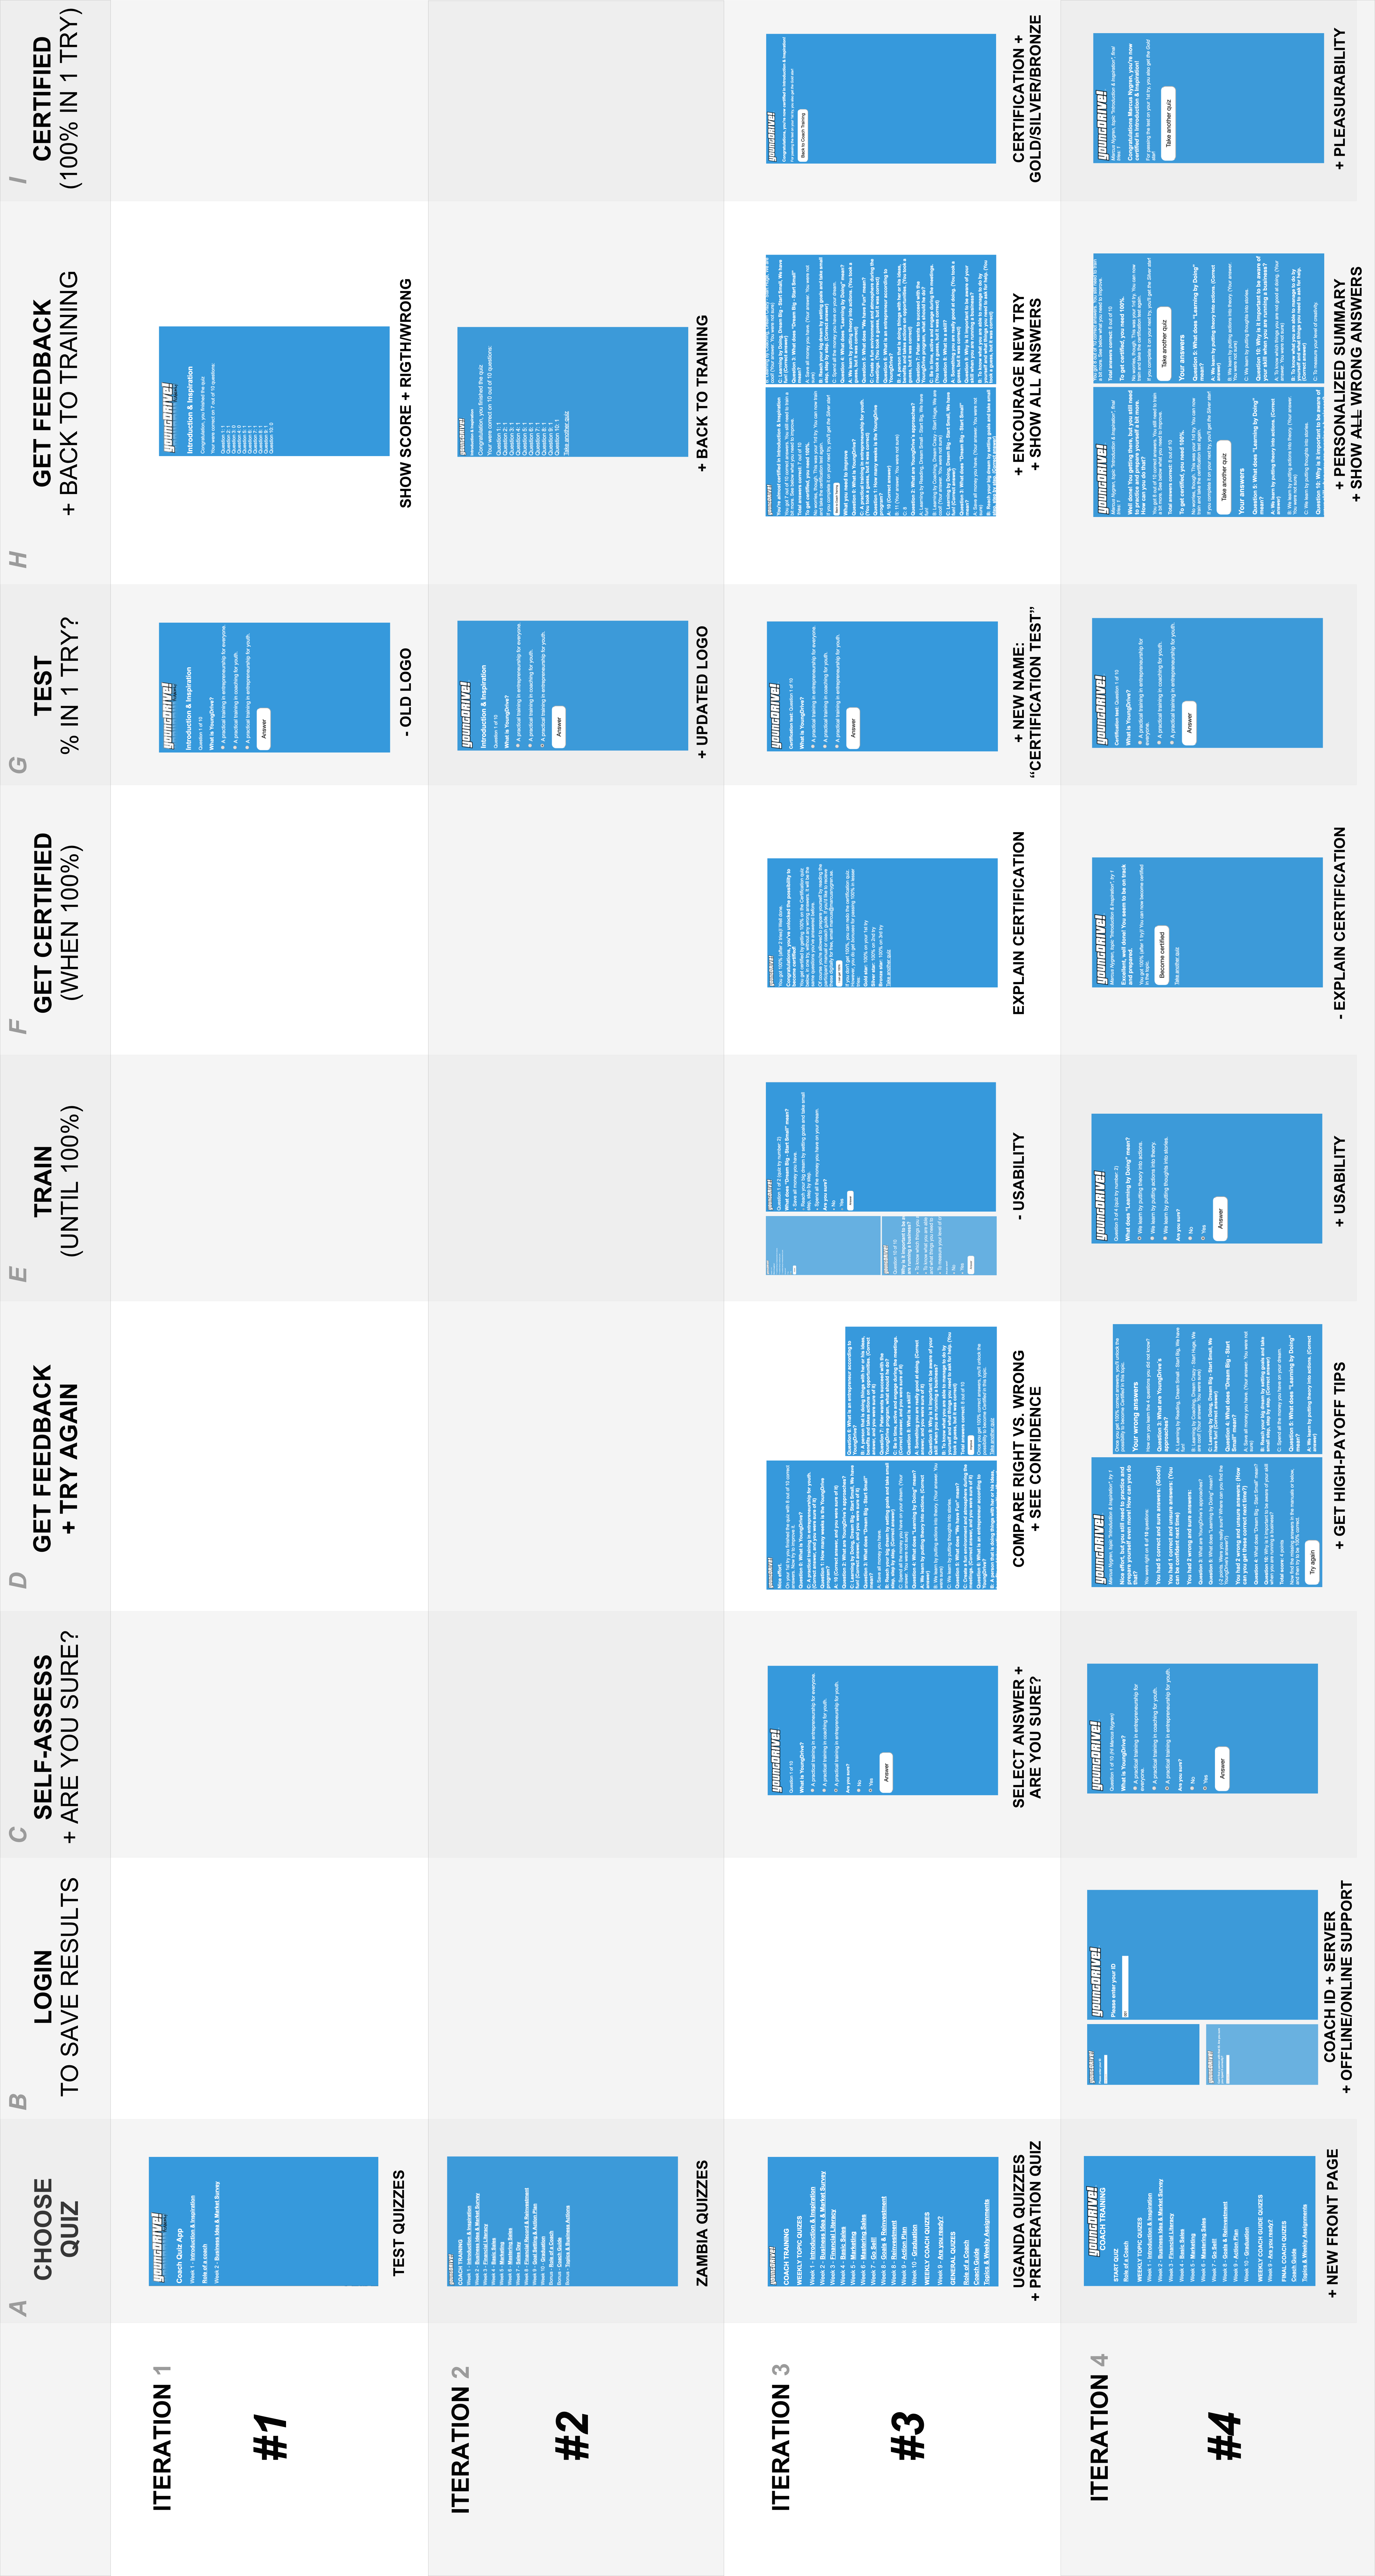
\includegraphics[width=1.0\textwidth]{IterationMapLowRes.png}
    \caption{The app flow described as a timeline (A-I), per iteration (1-4). E.g. in iteration 4, login (B4) appears after choosing quiz to take (A4).}
    \label{fig:iteration-map}
  \end{figure}

  %\subsection{Iteration \#1}

  There was no developed application at this point.


  The quiz flow during iteration 1-2 was a standard multiple-choice quiz game, designed for assessment, but not for learning. In a scoreboard, they could see which questions they were awarded points for and not, with a total score, see figure \ref{fig:iteration-map} H-1. In the end of iteration 2, whey were encouraged to go back to the start screen, to redo the same quiz again, or select a new one. 1 point is awarded for correct answers, whereas 0 points is given for incorrect answers.

  In iteration 3, feedback for self-reflection was introduced. The coach answers Yes or No on "Are you sure?" for each question (figure \ref{fig:iteration-map} C-3), with the aim of increasing meta-cognitive skills, and being able to give personalized feedback in the score board.

  Thanks to recording both if they were correct and confident, the app can give very precise learning feedback (e.g. showing that the coach answered alternative B with confidence, but showing that A was actually the correct alternative).

  In iteration 3-4, after observing their incorrect answers, and learning their correct ones (closely compare figure \ref{fig:iteration-map} D-3 and E-3), they could retake the wrong answers immediately.

  In iteration 3, the score board was simply showing each correct question with the answer the coach provided versus the correct one. After giving feedback, the coach can train, and improve on incorrect answers and guesses, and when being 100\% correct and confident, ideally take the whole quiz without faults.

  For iteration 4, the score board is more personal, encouraging the coach to reflect on her own learning process. The feedback is designed to give a self-confidence boost ("You were correct, and you were sure" or "You guessed, but you were correct. You can answer with confidence the next time"), unlearn knowledge ("You were incorrect, but you were sure"), or encourage studying more when unsure and wrong ("You were incorrect, and you were not sure").

  To discourage guessing during training, since iteration 3, the coach is shown number of tries on the quiz if they do not get 100\% in their first try (see the top bar of figure \ref{fig:iteration-map} E-3). For iteration 4, the coach will also get a minus point (-1) for answering incorrectly but confidently "Are you sure?": "Yes". If uncertain, the coach should answer "Are yo sure?": "No", and no penalty will be given. The coach will later recieve feedback, either "You can be confident next time" (if correct but unsure) or "How can you get these correct next time?" (if unsure and incorrect).

  The coach is encouraged to be well-prepared before trying again (either consulting the answers or the manuals). At 100\% correct answers, they can get certified, by getting the whole quiz correct without faults. Failing a question on the certification would show that they have not \textit{reliably} learned all the answers during the training. The more effort the coach has put into the training, the more likely the coach will be to pass the certification.

  %Lena Tibell menade vid förslaget att "Belöna inte hur snabbt %en elev går från att kunna till att inte kunna, för olika %människor lär sig olika snabbt". "Vad vi ville åstadkomma %med Antal försök var endast att undvika gissningarna".

   This certification quiz is the same as in training, but no longer do they need to answer "Are you sure?". If the coach can again get 100\% correct answers, without any faults, they have proved they are correct and confident with the topic they should teach the youth.

   If they fail a question, the score board will encourage more training and that they did not get certified, see figure \ref{fig:iteration-map} H-4. Since the coach did get 100\% correct in the training (maybe after a couple of tries) but not in the certification, the knowledge can be described as "Can do with effort". The coach can choose to take a new quiz, or take the same quiz from the beginning of the training.

   For passing the certification on the 1st, 2nd or 3rd time the coach is awarded a Gold, Silver or Bronze medal respectively (after certificate try 3, no medal is given, only the certificate). Compare figure \ref{fig:iteration-map} I-3 to I-4: for iteration 4, the "certificate" mentions the persons name and the topic certified in, which is a form of gamification in addition to the intrisic motivation of rewarding deliberate practice.


In the following sections, you can read more about what data guided the development of the final app, as well as the results from the final app evaluation.

\section{Iteration 1: Uganda Coach Visit}

Here the results from the qualitative and quantitative data for iteration 1 are shown, together with conclusions.

\subsection{Qualitative Data}

Below, the most important results from the stakeholder and coach interviews are presented.

\subsubsection{Stakeholder Interview Findings: Entrepreneurship Education Considerations}
Through early interviews with YoungDrive staff, it is clear that YoungDrive's entrepreneurship education methodology goes hand in hand with the presented theory. It's mottos are: "Dream big, start small", "Learning by doing" and "We have fun!" \citep{youngdrive-manual}. The YoungDrive program seems to be very appreciated by every party, especially the project partner, Plan International. The interviews with Plan International (see figure \ref{fig:stakeholderInterview}) showed great knowledge about YoungDrive's positive effect on the youth.

\begin{figure}[h]
  \centering
  \includegraphics[width=0.8\textwidth]{iteration1/stakeholderInterview.jpg}
  \caption{Meeting with Plan from the office in Tororo, making final preparations for the meetings.}
  \label{fig:stakeholderInterview}
\end{figure}

Both in regards to designing for the users and for the above reason, the app should be a complement to YoundDrive's existing training material and the structure of the program.

A challenging part of the work is that YoungDrive consists of both the practical skills of the entrepreneur, theoretical material of running a business, and an entrepreneurial mindset. Therefore, both how to assess knowledge, and build habits, needs to be examined.

As the stakeholder interviews answered "What's it like being a coach?", their perspectives could now be understood and summed into a early understanding of the coach situation. The stakeholder interviews heavily informed the Questionnaire guide, highlighting aspects that had previously not been taken into account.

\subsubsection{Coach Interview and Field Visit Findings: Teaching with Confidence}

The purpose of the coach interviews and observations was to understand "What's it like being a coach?", from the coaches own perspective. Thanks to having similar interviews with stakeholders, the coaches' opinions and experiences could be compared. Also, more detailed answers on background, desires, experience and situation could be provided.

 From the interviews and observations it was understood that CBTs can be responsible for from 7 up to 12 different youth groups in different programs, and such a high number places huge demands on the CBT. Even if there are only 7 groups, being behind on schedule or not being confident, can be very demanding.

%\textbf{Stayover at Patrick:} På morgonen visade Patrick mig hur han jobbar med deras tomt, var det odlas ris, och andra råvaror, deras djur, deras story från Syd-Sudan, till Kampala, till hyddan här i Tororo, och hans värderingar.

%Efter en ungdomssession nästföljande dag besökte vi och hälsade kort på en av de 2 CBT:s vi har session med idag. Sedan hade jag och Patrick den obligatoriska review av ungdoms-sessionen, och jag bjöd honom på middag. Kl. 19 ringde hans fru (som har börjat få tecken av malaria) och skyndade hem.

%Nästa ungdomssession fick jag besöka en annan CBT. Vi var tidiga. Sedan började jag prata med henne, och fick bra tillfälle att intervjua henne och även förklara för henne vad jag gjorde där. Det blev underligt att förklara för henne: Patrick påminde, när jag tabbat mig, att “Marcus, du måste förklara för X vad en app är”. Så hon fick låna min mobil, och jag förklarade att app var kort för applikation, och att för varje applikation har ett eget syfte, t.ex. ta foton. Jag bad henne klicka, svårt, råkade klicka åt henne, men sedan lät jag henne göra. Efter hon sett att det hon såg i skärmen var det hon såg på riktigt, blev hon jätteglad och började fundera vad hon skulle fota. Hon reste sig och gick runt hörnet, och jag följde efter. Hon fotade, efter att noggrannt tänkt igenom, att hon fotade buskarna med frukt. Sedan sade jag hon kunde fortsätta fota, och då tog hon ett litet runt hus utanför.

The interviews and observations with CBTs, Project Leaders and stakeholders led to the realization that different coaches handles this differently well. All coaches possess high self-confidence in varying degrees in various situations, and as a result, quality among coaches is unbalanced, which stakeholders see as a challenge. Depending on the situation, everything is going according to plan, you are not confident, or you are falling behind with the schedule, you can be in one of these three Need groups:

\begin{itemize}
  \item The ideal coach
  \item The realistic coach
  \item The challenged coach
\end{itemize}

It was discovered that coach confidence comes largely from being able to have good youth sessions, see figure \ref{youthSession1}. This is important, because according to the interviews, being a high-quality YoungDrive coach to a large extent means having high-quality youth sessions. For having a high-quality youth session, these are the most important attributes:

\begin{itemize}
  \item Correct information
  \item Correct structure
  \item Time management
  \item Fun atmosphere
\end{itemize}

\begin{figure}[h]
  \centering
  \includegraphics[width=0.8\textwidth]{iteration1/youthSession.jpg}
  \caption{Observing a youth session, the coach using the whiteboard to make certain concepts more clear.}
  \label{fig:youthSession1}
\end{figure}

These findings were used to inform the Customer Journey Map workshop. In addition to the findings here, questions were also asked around etnography.


\subsection{Quantitative Data}

    %What the data said

    Two workshops were held, which together would inform future development of an application. These were the findings from those two workshops:

    \subsubsection{Customer Journey Map: "A Day As a Coach"}

    The first workshop had the tree interviewed coaches as participants. See figure \ref{fig:cjm}. A Customer Journey Map would be created, with the purpose to understand all activities involving “A day as a coach”. The structure of the timeline was: “Before”, “During”, and “After” a youth session. Too understand how these activities differentiated between different coaches, three Personas were co-created based on the previously dicovered types of coaches: "the ideal coach" (John), "the realistic coach" (Joan), and "the challenged coach" (Suzan).

    \begin{figure}[h]
        \centering
        \includegraphics[width=0.7\textwidth]{cjmWorkshop.jpg}
        \caption{Two local project leaders and one coach mapping out the activities a coach does before, during and after hosting a youth session, in what is called a Customer Journey Map.}
        \label{fig:cjm}
    \end{figure}

    %After the 15 minute introduction, they started with 5 minutes + 10 minutes discussion mapping out Before, During, After for the ideal coach, John. Green postits were used.

    %Since it took too much time to do this for the other two personas, they were given 5 minutes to either use pink post-its for steps that a realistic coach would skip, and yellow notes that the coach would do differently. This worked well, and the results were discussed within the 5 minutes between the coaches, and explained during 5 minutes witth audio recording.

    %Since they were understandingly tired, they were given a 10 minute break, during which time they were asked to think about things that could go wrong for the sad/angry persona, Suzan. When I got back from the toilet, they had already started working! I took time of 5 minutes, and they walked through the concerns and it’s effects, just like they had did with the 2nd persona.

    They understood the concept of the workshop surprisingly effortlessly, although the concept of postits and Customer Journey Map and Personas were unfamiliar to them. Contributing to the energy, was probably that the timeline and personas were largely informed by their interview answers. The workshop gave great insights for understanding the coach situation and the coaches themselves, both observing their behaviour during the workshop and learning about all the unknown activities involved in being a coach.

    The first workshop was finished with many important insights. Thanks to using Personas, it was discovered from the workshop that the difference between coaches and the quality of the youth training was more diverse than originally thought.

    This is especially true when the coaches prepares for their youth session, an activity which was regarded as important as the coach training, but where quality of preperations were very divergent. This could be a great opportunity for delivering the app's promise of distance learning (see section \ref{purpose}). The teacher Josefina in an after-interview commented that while she can influence the coach training by her physical presence, she currently has no influence or insight into how the coach prepares, more than the co-project leaders' reports. When preparing for a session, there is a wide variety of \textit{when} the planning happens, and how a coach judges what amount of preparation is enough.

    Most coaches plan their next session during the morning, or immediately after a session with their group. Since a coach has somewhere between 7-10 groups (some even more), and the youth groups are at different modules, there is a lot of knowledge for the coach to handle - not only theoretical knowledge, but also the struggles of the youth, assignment presentations, workshops to be facilitated, etc. It is easy for a coach not to do everything as planned or as specified in the manual. Most of the coaches are said to be motivated by the possibility of becoming a better coach.

    According to the workshop, most of the coaches assess if they were ready for a topic \textit{after} a youth session. The feedback from the youth, as well as their questions and how well the coach can answer these, are the biggest informant. The exception is if the local project leaders comes to visit the youth session, but they do seldom have time to visit all of the coaches during a month, and during a month coaches should have taught 4 topics to all of their groups.

    \subsubsection{Smartphone Test using Quizoid and Duolingo}

    Quizoid (see figure \ref{fig:quizoid}) and Duolingo (see figure \ref{fig:duolingo}) were tested to understand the technical possibilities of the coaches, see figure \ref{fig:smartphoneTest}.

    \begin{figure}[h]
        \centering
        \includegraphics[width=0.7\textwidth]{quizoid.png}
        \caption{Quizoid is a simple multiple-choice game \citep{quizoid}, tested by coaches in iteration 1}.
        \label{fig:quizoid}
    \end{figure}

    \begin{figure}[h]
        \centering
        \includegraphics[width=0.7\textwidth]{duolingo.png}
        \caption{Duolingo is a praised app for language learning \citep{duolingo}, tested by coaches in iteration 1}.
        \label{fig:duolingo}
    \end{figure}

    \begin{figure}[h]
        \centering
        \includegraphics[width=0.7\textwidth]{iteration1/smartphoneTest.jpg}
        \caption{Picture from the smartphone test, observing how the coaches act using Duolingo and Quizoid}.
        \label{fig:smartphoneTest}
    \end{figure}

    Two of the three test users used a smartphone for the first time. The attitude towards using a smartphone was overwhelmingly positive. One of the coaches even mentioned: "Marcus, today one of my dreams have gone true." He even asked if he could borrow one of the devices during the remainder of the stay. Even for coaches that had never touched a smartphone before, some concepts were easily understood (like using the camera and Quizoid).

    Other concepts were harder (accidently getting to the settings menu, unlocking the device, understanding advanced games, or training languages using Duolingo with advanced interactions). Point and click is easily understood, whereas sliding is much more unnatural.

    The result was that the app can place itself somewhere in the middle of the two, regarding difficulty level.

\subsection{Discussion}

During a evaluation meeting with Linköping University and YoungDrive, it was determined that Iteration \#1 did provided answers for research question \#1, \#2, and \#3, and partly \#5. Thus, the iteration could be considered very successful, and now, the development of the app could begin.

It is clear from the data that the motivation of the app should be to assess and strengthen the entrepreneurship knowledge and skills of the coach. For coach quality to improve was a desire from the stakeholders as well as the coaches themselves, even if they were also satisfied with the current results. This lead to a challenging situation how an app can address becoming a better-performing coach.

An app could increase accuracy of correct information. With an app, the coach could keep a record of the module content, and see when and if they do need to refresh their skills. It was discovered that a coach app can benefit not only the coach training, but also in a surprisingly precise way, what was called "distance learning" in section \ref{purpose}. Accountability if the coach is ready for a session by automatic assessment. A very important aspect to increase learning and confidence will be to give good feedback (see section \ref{learning-assessment}).

With all the possible benefits of an app, it is definitely a problem that so few coaches have smartphones. Either continued development could be guided solely by the use case of having an app tailored for the coach training (where donated devices are available). But this would be to ignore that an app helping the coach to prepare for a session would be extremely beneficial, which discovered during the field visits to youth sessions and during interviews.

The motivation for using technology is very high, so one way forward would be that the app for distance training will reach only the users that can be given access to a smartphone, counting that more coaches will get smartphones in the future. Not using smartphones but feature phones (which all coaches possess), would mean building an SMS-based service (see \ref{rq1}.

As most coaches are already motivated to become a better coach and using technology, Sierra's \citep{sierra} advise of designing for their compelling context can be followed. From a YoungDrive perspective, this might mean "Given a teaching situation among the youth group, a great coach can teach an entrepreneurship topic more consistent with what the coach material said". Their performance in the YoungDrive app could translate into: "Given a question in the app, a great coach will get the right answer more often, and increasingly leverage the correct answer to their coach situation".

\subsection{Next iteration}
It is agreed with Josefina that the most important found skill of a YoungDrive coach is having great youth sessions. It is a challenge that the coach surely needs to feel, but does not always possess, self-confidence for its youth session. This partly stems from the lack of practical experience being put into realistic situations during the coach training.

If self-confidence comes from being able to deliver Correct Information, Correct Structure, Time Management and Fun Atmosphere, an app strengthening these will surely improve youth session quality. According to Josefina, assessing and increasing Correct Information is the parameter she values the most highly, and this will be the continued primary focus of the master thesis.

It is agreed with Josefina that preparing for a youth session can have an increased focus. It is a worry that designing for both the coach training and preparing for a session might be too ambitious within the given time frame. If so, designing for the coach training is deemed more important.


\section{Iteration 2: Zambia Coach Training}

Here the results from the qualitative and quantitative data for iteration 2 are shown, together with conclusions.

\subsection{Co-Creation Workshops}

There were two workshops held with the Zambia coaches: one at the beginning of the week (before being shown the app), and one at the end of the week (after having used the app for a week). Below, the learning from these two workshops are presented.

\subsubsection{Co-Designing an App for the YoungDrive Training}

    The result gave an unbiased look at what the coaches expected from the app, what functionality wasn't important, and into their technical preferences. A simpler design than originally thought was deemed sufficient, and the simple sketches guided continued development of the app during the week. See figure \ref{fig:zambia1A2}, \ref{fig:zambia1B2}, \ref{fig:zambia1C0} and \ref{fig:zambia1C1} for reference. The time spent on designing the YoungDrive app in two iterations took the coaches circa 1 hour and 40 minutes.

    \begin{figure}[h]
        \centering
        \includegraphics[width=0.9\textwidth]{workshops/zambia1A2.jpg}
        \caption{The design proposal from team 1}
        \label{fig:zambia1A2}
    \end{figure}

    \begin{figure}[h]
        \centering
        \includegraphics[width=0.9\textwidth]{workshops/zambia1B2.jpg}
        \caption{The design proposal from team 2}
        \label{fig:zambia1B2}
    \end{figure}

    \begin{figure}[h]
        \centering
        \includegraphics[width=0.9\textwidth]{workshops/zambia1C0.jpg}
        \caption{The design proposal from team 3, part A}
        \label{fig:zambia1C0}
    \end{figure}

    \begin{figure}[h]
        \centering
        \includegraphics[width=0.9\textwidth]{workshops/zambia1C1.jpg}
        \caption{The design proposal from team 3, part B}
        \label{fig:zambia1C1}
    \end{figure}

    From using the devices during the workshop (to find inspiration from other apps like Duolingo and Quizoid), it was found that most coaches prefer using the tablet (5 for tablet, versus 2 for smartphone and 2 for computer). Both the designs and insights gained were used throughout the week to further improve the simple app created at the end of iteration 1. The workshop gave great insights to who the coaches were and their thinking.

    \subsubsection{Understanding what Builds Confidence among Coaches}

    During this workshop, the focus was to examine what builds confidence among the coaches. Four themes were identified, after clustering the notes according to similarities: "I believe in myself" (3 coaches), "I believe in God" (2 coaches), "I am well prepared" (4 coaches) and "I am certified" (1 coach). See figure \ref{fig:zambiaWorkshop2} for the different clusters. Josefina comments after the workshop: “I have a problem: There is no way I can control them how they have prepared themselves for a youth session.".

    \begin{figure}[h]
        \centering
        \includegraphics[width=0.9\textwidth]{zambiaWorkshop2small.jpg}
        \caption{The clustered postits with needs, together with included design proposals.}
        \label{fig:zambiaWorkshop2}
    \end{figure}

\subsection{Quiz Results and Quiz Usage Observations}

    %What the data said

    Here some of the quiz results are shown. This section also presents the results from the two workshops held, in form of lessons learned.

    \subsubsection{Quiz Results from the Coaches}

    Quiz results ranges from the worst on 24\% (getting 4/17 correct answers) to 100\% (which has happened on 52/101 instances, for all of the quizzes). Week 9 was undoubtedly the hardest quiz, with the topic being "Goal Setting and Action Plan" (17 questions, average being 76.22\% correct answers, 18 quiz results submitted). The easiest quizzes are week 3 "Financial literacy" (11 questions), week 6 "Mastering sales" (9 questions) and week 7 "Sales day" (3 questions), where all of the results are 100\%.

    There are some amount of coaches that have taken the same quizzes multiple times. From this, interesting conclusions can be drawn. Attending the lecture shows a 15.0\% average increase in quiz results, compared to an 12.8\% increase with simply taking the quiz two times. This shows that a lecture is still more effective than learning via the app.

    Time to finish a quiz took between 2 minutes to 33 minutes (3/4 quizzes that took longer than 25 minutes were on quiz 9, there is a correlation with number of questions). Most of the quizzes took under 5 minutes to complete, and results are always over 80\% for these instances. This shows that the coach had a high confidence with the answers. Similarly, all of the scores under 60\% has taken more than 20 minutes. This can be explained by that the coach is unfamiliar with the app or smartphone, and that the coach is uncertain of the answers.

    It is seen in the quiz results that the quizzes did get gradually more challenging, as the average of quiz scores gets lower after day 3 of training, when it was discovered was welcoming the quizzes to get harder.

    The quiz scores when quizzes are performed in group is very varying (from 24\% to 100\%), and it is observed that influence of another coach can lead both to a worse score than their individual average, and a higher score. It is interesting to see that the three coaches that have the worst average (67, 72 and 85\%) are also the ones that have taken quizzes the least times individually, and the most taking quizzes together with others. This may show that the app is more effective when used individually, and there seem no other connection to previous entrepreneurial activity or background.

    There are few correlations that can be made between the coach's background and experience, compared with quiz results or app behaviour. Nothing in the coach information distinguishes the worst 3 performers in the quiz. For the opposite, there is however a noticeable behaviour that being confident, having trained youth, leadership experience, business experience, care for community, care for oneself and confidence to take on many youth, almost guarantees a high quiz average (which demonstrates learning) and quizzes done (which demonstrates motivation).

    For coaches with 0-1 negative remarks during the interviews (n=6) compared to coaches with 2-4 negative remarks (n=4), their quiz average is but 2\% higher (87\% to 85\%). This is not significant, but this number is increased to 93\% (an 8\% increase) if the outlier from the group is removed (a coach which only did three quizzes with average of 57\%). In the future, more research could be done into comparing coach data with quiz results.

    %Comparing instances when coaches have taken a test before and after a lecture, the results are: 71\%to 100\%, 59\% to 74\%, 80\% to 86\%, 90\% to 100\%. Without the lecture, improvements has been from 80 to 90, 100 to 100 to 100, 90 to 90, 80 to 100, 90 to 100, 100 to 100, 86 to 100, 100 to 100, 90 to 100.

    \subsubsection{Lessons Learned from App Test Observations: Motivation}
Regarding motivation from the coaches, one coach wished the app to be available on the Google Play store immediately, so that "The app could be used on my spare time". Another coach, without a smartphone, said "I'll buy one", because the utility of the app seemed so high. There were also suggestions for improvements, like "The app should have notes, not only quesitions". Regarding usability, low resolution screens made the text be barely visible. This showed, that the app needed to be tested on a lot of different devices. This is particularly true, as on day 1, the coaches did not know how to zoom, which could cause accident refreshs, frustration or confusion. Even more importantly, the app needs to work offline! To be online on the phone is too expensive for the coaches, and too unreliable to give a satisfactory experience. Also, during testing, relying on internet can cause a lot of problems, especially if the teacher is alone.

When asked about what they thought about doing one quiz ("Graduation") as a pre-quiz (before the session), 10/10 said they liked doing the quiz before, and that it benefited their learning during the session. When asked why it helped, 10/10 said agreed on the statement "During session, it is easier to follow" and that "Giving the paper manuals before, scanning headings and pictures etc, would not help". So, using the quiz before the session increases learning, slightly decreases fun of the session, according to coaches. One of the coaches described it as "Fun and encouraging".

    It was also tested to work in group or individually. The ones who answered, said that you learned more individually (3/3), and more fun doing it together (3/3). Doing it together, was enjoyable as it was "Very easy because of using different minds" and "We can collaborate to do better". It can be argued that the quiz being easier is not a valid motivation, but describes the learning in the app as a desirable difficulty.

    When doing a post-quiz ("Goal setting") immediately afterwards versus at the end of the day (doing spaced versus massed learning), quotes were "I thought it was fun and challenging to do the quiz immediately afterwards", with another coach commenting "The mind was still fresh". After a discussion with the teacher, these were the results:

    %When asked on timing preference, 10/10 said it would be more fun to do the quiz immediately afterwards, not at the end of the day. The motivation, seemed to be that it was easier.

    %9/10, said they wanted to do the quiz afterwards. The outlier, said it would be better for learning doing it later.

    %After this comment, this was the distribution:

    \begin{itemize}
    \item 3/10 wants to do the quiz both before and after a session
    \item 1/10 wants to do the quiz before and at the end of the day
    \item 7/10 wants to do the quiz only immediately afterwards
    \item 10/10 wants to do the quiz immediately afterwards, and then again at the end of the day
    \item 7/10 wants to do the quiz immediately afterwards, and then a joined quiz with other topics at the end of the day
    \end{itemize}

    The high scores on using the app a lot indicates that they like the app. The teacher wants to listen to coach opinions, at the same time not spending more time than necessary on assessment.

Regarding motivation from the teacher, asking Josefina what would hinder her from using the app, she says: "Not doing data collection digitally works whenever they are 10 - but not with bigger numbers than that." Also, according to the final interview with Josefina, she does not wish the app to replace her. She enjoys teaching, thinks she has an important role, and suggests the app to be designed to support her and the coaches, not replace her. She acknowledges that bugs in the app was a hindrance to functionality, and that a lot of testing (both high-dose, and high-scale) is very important.

\subsubsection{Lessons Learned from App Test Observations: Learning}
Regarding assessing knowledge, coaches had surprisingly high quiz results, and at day 3 they wished harder questions when asked. The response was to give harder questions the other days, for example by introducing similar answers, and testing 4 alternatives instead of 3. This was appreciated. The app was later tested on a university student in Uganda after the Zambia training, both on early and later quizzes. The university student from Makarere University scored 100\% correct, in spite of not having any entrepreneurship training. This showed that guessing was possible, or that the quizzes were too easy.

The teacher Josefina commented that this might not be a problem, as the YoungDrive coaches are not as skilled with using a process of elimination, and had indeed scored lower results on average with the later quizzes. When testing the app with refugee innovators during Humanitarian Innovation Jam in Uganda, similar results to the YoungDrive coaches were found. She explains this by that the cultural context is different, and that thanks to coaches in rural areas not being equally educated and skilled with reasoning, the problem is not as big as could be. Josefina is very happy with the app, and reviewed the app in the following way to Plan International after the training:

"The (YoungDrive coach training) app is a great tool to measure how much the coaches learned and understood from the daily training; it provides a clear overview of what the coaches truly understood and what they actually still don’t completely understand. Based on that information I as a tutor can adjust the training for the following day to make sure that the coaches understand everything correctly. The app also works as a motivator for the coaches; it´s clearly reflect their own daily performances. If they score high they become very happy and satisfied, if they score low they are eager to check their wrong answers.".

A coach scoring only 9/19 showed the relevancy of the quiz, as Josefina did not think she would have discovered that the coach was lagging behind otherwise. In the data, it was observable that the coach had done well together with others, but 3/7 when done individually. Josefina said about the 9/19: "This is where a control group would be beneficial". "He is often passive during open questions, but active during the team exercises."

According to Josefina, if you have a high score, you are ready. If not, you need to redo the quiz. If you are 8/10 or lower, you are in the red zone. If lower than 10/10, they are not ready, the motivation being that what they don't know, they will teach in an improper way: affecting hundreds of youth. This is why Josefina thinks they should need all of the answers correct.

Up until now, merely Correct Information has been assessed, not the other three factors. The fact that the app already is appreciated with assessing Correct Information, makes starting to assess the other factors interesting. Josefina informs that Correct Structure, Time Management and Fun Atmosphere would be the most viable to test \textit{after} a youth session, not before. She notes, that \textit{some} assessment could be made via the app before a session. This could to be further investigated.

\subsection{Summary}

The app works for assessing Correct Information! Since the coach training app was said to most importantly test Correct Information, secondly Correct Structure and Time Management, the iteration was considered successful.

Regarding the workshop \# 2, for iteration 2 the focus had been to assess "I am well prepared", for the very purpose of building confidence, in regards to Correct Information.

The review from Josefina was: "The (YoungDrive coach training) app is a great tool to measure how much the coaches learned and understood from the daily training; it provides a clear overview of what the coaches truly understood and what they actually still don’t completely understand. Based on that information I as a tutor can adjust the training for the following day to make sure that the coaches understand everything correctly. The app also works as a motivator for the coaches; it´s clearly reflect their own daily performances. If they score high they become very happy and satisfied, if they score low they are eager to check their wrong answers.".

\subsubsection{Insights}

  \begin{itemize}
    \item The app works for assessment!
    \item Good for learning for the coaches
    \item A good indicator for Josefina
    \item A great way to scale the YoungDrive training in the future, both for online coach-training and the physical training
  \end{itemize}

After the meeting with the partner and expert group, the following was concluded from iteration \#2:

\begin{itemize}
\item The app is only working on assessment now, not for learning
\item The need for a field app still feels relevant (especially for sessions long since the coach training)
\item The potential for YoungDrive having online coach training is huge
\item Multiple-choice is flawed in its current form
\end{itemize}

The insights on learning needed to be considered:
\begin{itemize}
  \item Are coaches really learning via the app, especially learning to be better coaches?
  \begin{itemize}
    \item How can questions be formulated in a way that teaches entrepreneurship, which is so practical?
  \end{itemize}
  \item How can the current multiple-choice quiz app be improved, to:
  \begin{itemize}
  \item reduce guessing
  \item improve confidence
  \item encourage learning
  \end{itemize}
\end{itemize}

Discussing the importance of self-reflection after a youth session with Josefina, led to asking more of such questions in coach quizzes.

Josefina: “I have a problem: there is no way I can control them how they have prepared themselves for a youth session."

An app could be used, either before you start planning (to guide what you need to study the most on), or after you think you are ready (so you can assess and improve).

Focus for the next iteration:
\begin{itemize}
  \item Score higher on Bloom's revised taxonomy, while still including multiple-choice questions in the app.
  \item Design quiz app for learning, focus on field app (CI, CS, TM, FA), and design having an app that works stand-alone from the YD coach training in mind.
  \item Try the Power of Yet approach in the app ("growth mindset" approach of "Not yet", versus fixed mindset and assessment)
  \item Test if the app created in Zambia could work also in Uganda
  \item All the quiz questions would need to be converted from the new (Zambia) manual to the old (Uganda) manual, since both structure and content had changed.
  \item Josefina was given a task to create a quiz "Are you ready for Session 9?".
  \begin{itemize}
    \item partly to score higher on \textit{Bloom's revised taxonomy}
    \item partly to test if Correct Structure and Time Management could be assessed using multiple-choice
  \end{itemize}
\end{itemize}

\subsubsection{Findings}

Test with university student scored 100\% correct, means that common sense can go a long way, and that the results can't be 100\% trustworthy, and that multiple-choice questions has serious issues - this, we already knew during and before the coach training - but it needs to be taken care of.

The app would be great and could actually work outside the physical coach training - with revision, be stand-alone, even being able to distribute online.

Now there are observable evidence for what the interactions from Iteration 1 showed:

\begin{itemize}
\item The purpose of the coach training should be to prepare the coach in having great youth sessions
\item Therefore, this is what the quizzess should assess
\item What it really means being a good YoungDrive coach, is having good youth sessions
\item Josefina would have liked to be able to stop coaches from having taught, if they do not have 90-100 \% correct information on the subject
\item Today, Josefina can not assess this. This means that some coaches, are teaching incorrect information to hundreds of youth.
\item Here, the quiz has a very good need to fill.
\end{itemize}

With all of these findings in summary, it can be concluded that an app for coach training, and an app to use before a youth session, could be the same app, since the purpose of preparing the coach to be great with its youth session is the same.

From the interviews, it was learned that while it \textit{may} be technically possible, the teacher desires the app support her, not replace her.

To get an app suitable for learning, it was determined that the pedagogical model behind the app needed to change, emphasising feedback.


\section{Iteration 3: Uganda Formative Test}

Here the results from the qualitative and quantitative data for iteration 3 are shown, together with conclusions.

For the coach training in iteration 1, only assessment was okay, since Josefina could give feedback. But if assessing preparedness for a youth session, the app leaving the coach with not being ready is not viable. Given a coach having prepared for their youth session on week 9, and then only scoring 5/10, what should happen? In a similar way, what should happen if 9/10 correct answers? Clearly, if the coach has 9/10, this coach should get feedback to improve, and especially if the score has been 5/10.

\subsection{Qualitative Data}

  %What the observations said

  \subsubsection{Observations before going to Tororo}
  Before going to Kampala, because of the major changes to the app, the concept was tested with an entrepreneurship student in Kampala and the Zambia teacher, Josefina. The two tests informed that the app was now ready to be tested with the coaches in Tororo.

  The entrepreneurship student's overall opinion on the app was: "Can you give me the link, because I'd love to do more of this. I think it's amazing.". There were some issues found with phrasing: "Improve" should be renamed, because it is not intuitive what the button would do. The coach was also surprised that the certification did not include something substantial (meaning it felt hollow). The student would have preferred unlocking a business challenge (showing self-determination), or something where he could get a learning reward instead of a "well done" and a badge (showing the student was not motivated by achievement in itself), see figure \ref{fig:iteration-map} I-3). This test was very valuable, and gave early insight to how the Uganda coaches might act within the app.

  The teacher in Zambia, Josefina, was consulted to comment on the app. When asked for an opinion, Josefina answered: "I like the idea that when the coaches have answered all of the questions correctly, they can consilidate the knowledge by the certification test, when the coach should get 100\% correct on their first try." This verified the relevancy of the taken approach of separating Training and Certification.

  \subsubsection{Service Mini-Sprint - 5 workshops}

  For the following workshops, the coaches themselves could propose topics. These were the five most wanted topics, according to the coaches:

  \begin{enumerate}
  \item Finding the YoungDrive icon after unlocking the device
  \begin{itemize}
    \item The outcome led to in iteration 4, only the YoungDrive icon being on the start screen, and no other apps.
  \end{itemize}
  \item Making the app more user-friendly
  \begin{itemize}
    \item While the proposals was not very concrete, this led to a realization that the app needed to be more user-friendly, and thus gave a larger focus on this for iteration 4.
  \end{itemize}
  \item Finding local examples of entrepreneurs to inspire the youth
  \begin{itemize}
    \item This lead to the realization that most coaches having a hard time finding local success examples of entrepreneurs. An app could address this need in the future, both having a bank of successful local entrepreneurs, and booking them for visiting a youth session.
  \end{itemize}
  \item How to get access to smartphones (costing no more than ~70 USD)
  \begin{itemize}
    \item The action was very concrete: a Plan International staff voluntarily participated in this workshop, they contacted two retailers of smartphones, and concluded that 1) coaches could utilize the youth saving group to afford buying their own devices or 2) Plan International could buy and then borrow devices to the coaches, coaches being prepared to pay if they got lost or damaged. The results showed that both stakeholders and coaches are very eager to be equipped with smartphones, seeing the benefits.
  \end{itemize}
  \item Becoming a better coach via other apps (like Google's products)
  \begin{itemize}
    \item This workshop was very interesting, as coaches found numerous uses of a smartphone which would benefit them in their work. The coaches even figured out how to use Google voice to ask questions, like the most profitable company in Tororo, or getting directions, or using the app for translations. It is evident that equipping the coaches with smartphones has very concrete extra benefits other than the YoungDrive app, and shows a tendancy that the coaches are more eager to use the smartphone for utility than for entertainment.
  \end{itemize}
  \end{enumerate}

  \subsubsection{Field Visits}

  During field visits, 3 Community Bases Trainers were tested with the app, to observe usage of the app immediately after having prepared a youth session.

  Some things were notable from the interactions: %with John:
  \begin{itemize}
    \item "Are you sure?" is understood intuitively (you can't progress without answering), but some coaches deliberately answer "Yes" even if they are not sure.
    \item Idea to highlight different words of similar answers, to increase speed
    \item In summary, if wrong, show the other alternatives either way, not only the wrong answer
    \item Idea for future work: "Go to participant manual" within the app % Juliet, this was discovered:
    \item If correct and unsure, she says "I still feel good". "Include it in wrong, because maybe I was still guessing". (This later informed the Certification quiz-insight)
    \item Change button to "Become certified", to increase likelihood to press the button. As of now, it was not obvious.
  \end{itemize}

  When she did get certified, she said "I feel good". When asked why, she said: "They have appreciated what I have done". The next day, the same three CBTs gathered at the Plan International office to do an app test on the hardest quiz.

  Having a service mini-sprint after the field visit, quick iterations could be made to the app. One such example comes from the field visits. Originally, it was believed best to use Gold/Silver/Bronze in the Training mode, and "Are you sure?" in the Certification mode. User tests showed that the other way around was better, and this was changed for the next meeting with the coaches. This example shows the relevancy of testing the app with the intended users, as it had not been eveident from the tests with the Kampala student or the teacher.

  A service design approach was used, first observing how preparations was made without the app, and \textit{then} introducing assessment via the app, followed by interview. What was the most valuable feedback from the field visits, was to see that the app had indeed been a perfect fit for use in the field before a youth session. However, it was not possible due to time limitations to follow the coach to their youth session afterwards, to see the actual effect of preparing via the app.

  \subsubsection{Small Formative App Test}

  Several conclusions could be drawn from the app test with the three coaches. Two of the coaches were competing with finishing the coach guide quiz 9 (see results in figure \ref{fig:areYouReady}, while the third coach (who arrived late) offered feedback on the app.

  \begin{figure}[h]
    \centering
    \includegraphics[width=0.8\textwidth]{analysis/areYouSureQuiz.png}
    \caption{Data analysis in Google Sheets from the quiz results during the workshop for the coach guide quiz 9: "Are you ready?".}
    \label{fig:areYouReady}
  \end{figure}

  The two coaches did 17 quizzes on quiz 9. One was allowed to use the manual (Betty, coach ID 203), while the other could only consult the feedback via the app, see figure \ref{fig:iteration-map}, D-3 and H-3.

  Apart from the quantitative quiz results, some comments were made. Betty having 4/12 correct answers on the first question, when asked from the quiz question 13 "How comfortable and ready do you feel right now to carry out session 9? (There is no right answer, just be honest with yourself!)", answered " Ready, but I probably still want to look in the coach manual and participant manual.". The other alternatives were: "Not ready at all, I need to prepare myself more by using the coach manual and participant manual.", "Somehow ready, but I still need to look more in the coach manual and participant manual." or "Very ready and comfortable.".

  Betty got 4/12 correct answers on her first try, but eventually she did pass the certification, getting 12/12 correct answers in one try in 102 minutes from the quiz start. It took her 43 minutes from her quiz try 1 to passing the training. She then failed the certification try 1 (i.e. not getting Gold) after spending 17 minutes with it. thus, she needed to go back to the training. Back in the training, now she got 8/12 instead of 4/12, and passed the whole training in 17 minutes. Then, she got 12/12 in the certification test (earning Silver), in only 12 minutes.

  Juliet also got 4/12 correct answers on her first try. Not understanding the "Improve" button, she repeatedly went back to the home screen and retook the whole test (like in iteration 2). This was a slow approach. On her new tries, she got 5/12, 4/12, 5/12, which showed that learning was too hard. Similar results had been found in iteration 1 using Duolingo, where the app failed to train the coach to get a better score. After this try, she was explained the "Try again" button, got 7/7 (spending 22 minutes with the questions compared with her 16.25 minutes average doing all 12 questions, which showed she really put effort into analyzing the answers properly). Unlocking the certification test, she got 9/12 in 5 minutes, an improvement from 4/12 on her quiz try 1 75 minutes before.

  The results from this quiz shows that:
  \begin{itemize}
  \item "Improve", only needing to repeat the questions you are not sure of, does improve learning quality and speed, compared to retaking the whole quiz again after each try - it makes learning more focused on what you need to train
  \item It needs to be clearer that you should press "Improve", for example by changing the text to "Try again"
  \item The time needed to become reliant on the session takes too long. To pass the rule of thumb for deliberate practice, a session getting to 95\% reliability should take 45-90 minutes. For Betty, it took 102 minutes from quiz start to being 100\% reliable. For Juliet, she did only manage to get 75\% reliable within the same time frame. Either scaffolding needs to increase (dividing the quiz into smaller chunks), or learning effectiveness needs to increase (for example by better feedback).
  \end{itemize}

The data and observations also shows that learning Correct Structure and Time Management via multiple-choice is not effective. Especially, this is shown by the time it takes to get a high score. To score well on such a test, the coach would retrieve from memory using a clear mental image. In its current design, getting a clear mental picture is not supported from the multiple-choice design. See Future Work in chapter \ref{future-work} for a further discussion how this Correct Structure and Time Management can be better assessed in the future.

\subsection{Quantitative data}

    %What the data said

    \subsubsection{Big formative app test}
  The app test simulated the app being used to assess preparedness for a youth session. The test clearly showed evidence between the difference between designing for Assessment and Learning. See figure \ref{fig:summativeTest} and figure \ref{fig:computerTest} to understand the setting.

  Before the quiz started, the coaches were asked to raise their hand if they felt proficient with using a smart phone. 8 out of 23 said yes. After using the app, 16 thought they were proficient (25\% increase), while 5 said low proficiency, and 2 said no (we don't yet feel proficient, still fear).

  The test was done in pairs, because of lack of devices.

  \begin{figure}[h]
    \centering
    \includegraphics[width=0.8\textwidth]{appTestTablet.png}
    \caption{Two coaches using a tablet for the formative app test. The coaches worked in pairs. After the app test, interviews was held, before co-creation workshops started.}
    \label{fig:tabletTest}
  \end{figure}

  \begin{figure}[h]
    \centering
    \includegraphics[width=0.8\textwidth]{appTestComputer.png}
    \caption{A variation of smartphones and tablets were used. In one case, the battery died on one of the device so it needed to be replaced with a computer. It was the first time the coaches used a computer, and they learned quickly and eagerly.}
    \label{fig:computerTest}
  \end{figure}

  Regarding usability, the most negative thing from the app test, was that the app was not user friendly for 1st-time smartphone users. There were a lot of bugs, the most damaging for the app test being resizing of the font size for each new question, see figure \ref{fig:iteration-map} E-3. This forced some coaches to try to zoom on the devices, even if they did not know how. This could in turn cause refresh of the web page, and sometimes there was no Internet available. Thus, the data can not be fully reliable.

  This was the first time true frustration was shown. Out of 23 respondents, 7 rated the app easy, 11 medium, and 6 hard. This was not viable.

  Regarding learning, cognitive load seemed to be too high. The feedback was not scaffolded enough, so coaches did not have enough energy to assess all of their results carefully before taking the test again via "Improve". One user did not want to press "Improve" until having read the manual. The motivation was: "Not because that is what the info says, but because I can learn more from the manual, about more than what the questions says." This is in fact the preferred behaviour from Josefina, and the app should continue to further encourage only using the app training or certification mode after having prepared via the manual. This way, the app is still assessment, but it is "learning by thinking", with feedback. In iteration 4, comparing those that are allowed to use the manuals with those that are not allowed to, would be interesting.

\subsection{Sprint Demo}

  A sprint demo concluded the findings from iteration 3. Now the coaches could not only assess, but also \textit{learn} Correct Information, which was successful, but needs to be done more effectively. It took an unacceptable amount of time to reach 100\% proficiency on all the quizzes. This was especially evident, on the quiz on Correct Structure and Time Management, "Week 9: Are you ready?", when it took a coach 102 minutes to reach 100\% without errors. In iteration 2, when "Improve" did not exist, it probably would have taken even longer.

  For the first time both signs of learning via perceptual exposure (many questions during a limited time, by trial and error) and deliberate practice (via learning via reflection) could be identified from the app. It is just that the app as of now is quite inefficient, especially in terms of speed, so while the ideas are there, the criteria are not fulfilled.

  The focus had been on "I am well prepared", but also including "I am certified.". It was shown that most coaches do not care about the simple gamification aspect of "I am certified" (which the workshop already had shown) but that they do care about their learning progress and learning results. The app could further embrace this.

  If there is one thing additional learned during the iteration, it is the insight that data is knowledge, and knowledge is powerful. A realization is that both the developer, the coaches, the teacher, and the project partners can gain important insights from the data. Adding "Are you sure?" to each quiz question, coach understanding was amplified, because now, also the coach's attitude towards learning can be evaluated. See more about this in the Discussion chapter \ref{cha:discussion}.

  \subsubsection{Next Iteration}
  To improve effectiveness for the next iteration, a couple of goals were chosen. While the app would work well for the Ugandan coach training, the use case of a youth session was not good enough yet. Mostly, this is in regards to that it takes too long time to improve via the app, and that the feedback is not sufficient. This leads to introducing these forthcoming goals, with the associated recommendations:

  \begin{itemize}
    \item Improve Deliberate practice. The criteria for Deliberate practice is not fulfilled today.
    \begin{itemize}
      \item  Follow the recommendation to design so that knowledge in a topic can go from unreliable to 95\% reliability within one to three 45-90-minute sessions.
      \item If this is not possible from changing the learning tactic, don't continue trying: split the quizzes into smaller pieces \citep{sierra}.
    \end{itemize}
    \item Improve Perceptual expose
    \begin{itemize}
      \item Divide the learner's expertise according to \cite{sierra}, "Can't do", "Can do with effort", and "Can do effortlessly".
    \end{itemize}
    \item Increase the use of questions to prompt self-monitoring  and self-evaluation \citep{sitzmann}.
    \begin{itemize}
      \item Using "learning by thinking" and encouraging a growth mindset, can benefit reaching metacognitive skills on Bloom's Revised Taxonomy.
      \item Help the coach to analyze and evaluate its own learning, possibly improving faster in the app.
    \end{itemize}
    \item Improve feedback to reflect that the teacher does not want to encourage coaches to have their youth session before they are 100\% confident with the material
    \item Data collection should be online and needs to be individual, so that the data is increasingly without faults and can be more easily analysed
    \begin{itemize}
      \item To do it online means that there needs to be a database, but also a login, so individuals are traceable.
    \end{itemize}
  \end{itemize}


\section{Iteration 4: Uganda Summative Test}

Here the results from the qualitative and quantitative data for iteration 4 are shown, together with conclusions.

\subsection{Analysis of Interviews}

The answers given during the three group interviews has been summarized and clustered into three areas, see figure \ref{fig:overview}. Further, the answers within interaction design has been clustered into its four main principles, see figure \ref{fig:interactiondesign}. The questions regarding learning has tried to answer why a coach is correct or incorrect on a given question, see figure \ref{fig:learning}. Service design has been clustered into the two questions "When do you want to use the app?" and "When are you not able to use the app?", see figure \ref{fig:servicedesign}. Zoomed-in versions of all of the areas are presented after the overviews, where the analysis of the quotes can be seen in its fullest. The quotes from these mind-maps are individual, which means that if another coach has had a similar thought, their quote is branched next to the following quote.

\begin{figure}[h]
    \centering
    \includegraphics[width=0.3\textwidth]{analysis/interviews/overview_notexpanded.png}
    \caption{The interview answers has been clustered into three areas: learning, interaction design and service design.}
    \label{fig:overview}
\end{figure}

\begin{figure}[h]
    \centering
    \includegraphics[width=0.3\textwidth]{analysis/interviews/interactiondesign_notexpanded.png}
    \caption{The coach quotes regarding interaction design has been divided by four criteria: pleasurability, usability, utility and desirability.}
    \label{fig:interactiondesign}
\end{figure}

%For learning and service design, the analysis of the interview quotes can bee seen in its fullest in figure \ref{fig:learning} and figure \ref{fig:servicedesign} respectively. Zoomed-in versions of all of the areas are presented after the overviews, where the analysis of the quotes can be seen in its fullest.

\begin{figure}[h]
    \centering
    \includegraphics[width=0.3\textwidth]{analysis/interviews/learning_notexpanded.png}
    \caption{The coach quotes regarding learning has been divided by if they give insight to why a coach has been correct or incorrect on a given question.}
    \label{fig:learning}
\end{figure}

\begin{figure}[h]
    \centering
    \includegraphics[width=0.3\textwidth]{analysis/interviews/servicedesign_notexpanded.png}
    \caption{The coach quotes regarding service design has been divided into \textit{when} you want to use the YoungDrive app, and when you are hindered from doing so.}
    \label{fig:servicedesign}
\end{figure}

\clearpage

\subsubsection{Learning}\label{sec:interview-learning}

By reading the quotes from the coaches carefully, it can be understood why answers can appear correct by the coaches (see figure \ref{fig:learning1}), even if this would not be the case (see figure \ref{fig:learning2}.

\begin{figure}[h]
    \centering
    \includegraphics[width=1.0\textwidth]{analysis/interviews/learning_correct.png}
    \caption{Quotes explaining why a coach could give an correct answer on a given question. Either you were sure of the answers, or you made a qualified guess. A prerequisite for answering the question correct is that you understood the questions meaning.}
    \label{fig:learning1}
\end{figure}

\begin{figure}[h]
    \centering
    \includegraphics[width=1.0\textwidth]{analysis/interviews/learning_incorrect.png}
    \caption{Quotes explaining why a coach could give an incorrect answer on a given question. Either, the coach did not have sufficient knowledge to answer the question confidently (for a number of reasons, given in the figure), or the question was not understood correctly, or the app usability was a hindrance.}
    \label{fig:learning2}
\end{figure}

\clearpage

\subsubsection{Interaction Design}

Most importantly, in the final app test, everyone thought the app was good and easy to use (n = 26). This is important, as this had not been the case in iteration 3. Regarding the four different areas of interaction design, positive remarks on utility are especially beneficial for learning. However, pleasurability, usability and desirability is a prerequisite for the app to be used by the coaches. For desirability, if the coaches are stimulated by using the app, two reviews were: "It felt good using the app" and "It motivated learning". The other three interaction principles (pleasurability, usability and utility) have been given their own mind-map below, see figure \ref{fig:interaction1}, figure \ref{fig:interaction2} and \ref{fig:interaction3}.

\begin{figure}[h]
    \centering
    \includegraphics[width=1.0\textwidth]{analysis/interviews/interactiondesign_pleasurability.png}
    \caption{Pleasurability was 100\%, as the app had a good design and well-motivated questions, however some coaches were frustrated by difficult questions in the app, or the time needed to complete a quiz during the workshop.}
    %From the interviews, it is visible that the coaches feel the quizzes has been a fair way to measure their knowledge in the topic. The answer "It leads to confidence" could show that when a coach has done a quiz reaching certification, they do feel more confident about teaching the topic.
    %Positively, assessment of "Am I ready?" can happen already before the youth session, in the app.}
    \label{fig:interaction1}
\end{figure}

\begin{figure}[h]
    \centering
    \includegraphics[width=1.0\textwidth]{analysis/interviews/interactiondesign_usability.png}
    \caption{Usability. As previosuly stated, all of the coaches (25/25) thought the app was easy to use when asked by raise of hands. However, in the interviews, some detailed comments regarding usability appeared. Regarding workshop issues, some of the devices' battery died during the workshop, or needed to be replaced. Regarding the app, some still mention too much information to appear at once, or that information are shown that the coach does not expect. Only one coach mentioned thinking that thee login was not user friendly, since the Coach ID was easy to forget. The Coach ID has since been documented by the local project leaders, so they can be contacted in such situations.}
    \label{fig:interaction2}
\end{figure}

\begin{figure}[h]
    \centering
    \includegraphics[width=1.0\textwidth]{analysis/interviews/interactiondesign_utility.png}
    \caption{Utility gives a valuable measure of what benefits the coach finds with using the app. Quotes regarding usefulness are: "It quickens the exercise", "It carries all summaries of the work", "It reminds to guide the youth correctly". For training, coaches conclude that "It evaluates my performance" and that "The feedback is excellent". One coach summarizes with "It increases the level of perfection".}
    \label{fig:interaction3}
\end{figure}

\clearpage

\subsubsection{Service Design}

It is important to understand if and when the app will be used by the coach, and if the environment of the coach in any way can hinder use of the app. For understanding the coach situation to these two criteria, see figure \ref{fig:servicedesign1} and \ref{fig:servicedesign1}.

\begin{figure}[h]
    \centering
    \includegraphics[width=1.0\textwidth]{analysis/interviews/servicedesign_when.png}
    \caption{There are very varying answers to the question "When do you want to use the app?". Most coaches would have liked to use the app immediately. Some of the coaches identified the need for devices, more training, or charging of devices in being able to do so.}
    \label{fig:servicedesign1}
\end{figure}

\begin{figure}[h]
    \centering
    \includegraphics[width=1.0\textwidth]{analysis/interviews/servicedesign_cant.png}
    \caption{Answers for the question "When are you not able to use the app?" are grouped into four segments: internet issues, battery issues, low or no access to smartphones, or if the app is not usable because it is not available on the smartphone, or the coach does not know how to use a smartphone.}
    \label{fig:servicedesign2}
\end{figure}

\clearpage

\subsection{Analysis of Quiz Results}

    %What the data said

    % Christine och Patrick berättade senare att i regel presterar Young Mentor lite bättre än CBT, enligt deras rakningar. (från iteratoin 1 - stämde detta?)

    % Relevans av att testa financial literacy: "Precis som med förra gruppen, verkar ekonomin vara det svåraste att förstå (dolda utgifter, hur gå med vinst), som youth." (från iteration 1)

% Important to be objective
% En diskussion om hur resultaten kan användas i praktiken är också i de flesta fall belysande och relevant i rapporter

% https://liu.se/ias/kontakta-oss?l=en

For the first time, automatic data collection was used, which increased the amount of quantitative data that could be analysed substantially. Below, the findings from each data analysis method are presented. There was one test group and one reference group, the difference being if they were allowed to consult the manuals or only use the feedback from the app.

\subsubsection{Quiz Results and Pre-Test Data Analysed in Google Sheets}
For results gathered and analysed within the Google Sheet, see figure \ref{fig:analysFarg3}. For a zoomed in version, see Appendix \ref{cha:appendix4}. Early observations from the pre-test data when inserted into Google Sheets was that a surprising number of cells were left blank. One user had not done the pre-test (see column for coach 220), where some had left questions unanswered (most commonly "Do you own a company?" (should have used the word "business"), plus "Hours of preperation" and "Occations for a youth session" (there is a tendency this might be because they were not proud of their answers, because of correlations with low quiz results).

\begin{figure}[h]
    \centering
    \includegraphics[width=1.0\textwidth]{analysis/sheets/0Overview.png}
    \caption{The Google Sheet after merging the pre-test data and the summed quiz results data. See zoomed-in versions and explanations for each section below.}
    \label{fig:analysFarg3}
\end{figure}

\begin{figure}[h]
    \centering
    \includegraphics[width=1.0\textwidth]{analysis/sheets/1Pre-data.png}
    \caption{Pre-test data}
    \label{fig:1Pre-data}
\end{figure}

\begin{figure}[h]
    \centering
    \includegraphics[width=1.0\textwidth]{analysis/sheets/2Quiz3.png}
    \caption{Quiz 3 answers.}
    \label{fig:2Quiz3}
\end{figure}

\begin{figure}[h]
    \centering
    \includegraphics[width=1.0\textwidth]{analysis/sheets/3Quiz9A.png}
    \caption{Quiz 9 try 1 answers (correctness and recorded confidence ("Are you sure?": "Yes/No") on coach guide quiz 9 "Are you ready?", together with answering "How comfortable and ready do you feel right now to carry out session 9? (There is no right answer, just be honest with yourself!", alternative 1-4 ("Not ready at all", "Somehow ready", "Ready" or "Very ready and comfortable"). Finally in column Y, the time it took for the coach to complete quiz try 1 is given.}
    \label{fig:3Quiz9A}
\end{figure}

\begin{figure}[h]
    \centering
    \includegraphics[width=1.0\textwidth]{analysis/sheets/3Quiz9B.png}
    \caption{Quiz results on the training and certification of coach guide quiz 9 "Are you ready?". Column AB: how many minutes they spent in training. AC: how many times they pressed "Try again", retaking the wrong answers. AD: their score on the last training quiz they took. AE: the increase from their first training to their last. AF: recorded "Are you sure?": "Yes/No" after taking the quiz try 1. Finally, for the coaches that started the certification, their results are shown, together with the time the quiz took for those that got 100\% correct on the first try.}
    \label{fig:3Quiz9B}
\end{figure}

\begin{figure}[h]
    \centering
    \includegraphics[width=1.0\textwidth]{analysis/sheets/4Pretest.png}
    \caption{Pre-quiz results per question and coach. The correct answers are given in green. The questions asked can be observed in Appendix \ref{cha:pre-test}}.
    \label{fig:4Pretest}
\end{figure}

\clearpage

Missing cells was not as obvious with the app results, were users could not progress in a quiz without answering both the question and the confidence. However, none of the passed quiz 9 certification answers had been submitted. Thus, it was needed to add these from the manual recordings, which had been used as a backup in case anything like this would happen.

There were a number of quick insights that could be drawn before the parallel coordinates visualization, simply by looking at the data as a spreadsheet.

It was believed that smartphone users feeling like novices might have a disadvantage with the app, since they will not learn as fast as experienced users. The interactions shows however, between iteration 3 to 4, almost all of the coaches does not feel intermediate instead of beginners using the smartphone and the YoungDrive app. The quiz data verifies this, with no direct correlation between technical skills and quiz results (comparing column H "Smartphone level" 1-3) with column M and T (quiz scores on the first try for quiz 3 and 9). From the pre-test data, it can be seen that only CBTs said they didn't feel comfortable with smartphone (n=2, column H, of which there were 6 Youth Mentors and 14 CBTs). A reason might be age, as CBTs were older than the Youth Mentors. Also, youth mentors had higher school level than the CBTs. More probable, is that the experience of using a smartphone since iteration 3 has matured over time, and that they are now more confident. %It is interesting that this has improved since iteration 3, possibly indicating that the smartphone skills have matured since the last test two weeks ago.

From the Google Sheets quiz results data, it could be seen that there was a surprisingly low number of answers where the user answered the question without confidence (see column P, U and AF). This is not good for feedback purposes, as answers were actually often not correct.

First-hand insights before the parallel coordinates were that there was a strong correlation between pre-quiz results (column D) and quiz 9 try 1 (column T), and slightly visible also in quiz 3 try 1 (column M), but with more outliers. Also, with manuals there was a higher probability of finishing quiz 9 training and certification (see also findings from the parallel coordinates visualization below). The data shows small tendencies that being honest and deliberate during the training increases the likelihood that a coach can get 100\% without faults, and has truly learned.

The final version of the app shows users can get 100\% on quiz results much faster (column R, AB and AI) than the previous version, as the score board had been improved for iteration 4. Since the target group in Zambia and Uganda was different, it is hard to empirically prove if it went faster getting 100\% with the possibility of repeating only the wrong questions, asking "Are you sure?", and providing individual feedback. Asking after the app does in iteration 4 does show however, that 100\% of the coaches now thought the feedback was good for learning.

%\subsubsection{Bonus Result: Learnings from Observing All of the Quiz Results}
Also, from observing all of the quiz submissions (see sample in figure \ref{fig:unprocessedData}), more users had started a quiz without finishing it than anticipated. This speaks for usability issues (cancelling the quiz by mistake, like clicking the back button, or loss of internet access) or bad technical skills (needs to design to be more fail-safe) or lack of motivation (needs to design for unmotivated coaches as well. The need group of "challenged coaches" might need other design than "ideal coaches".

Finally, a lot of users had done quizzes that were not Topic quiz 3 and Coach quiz 9, which might indicate high interest (if they did more than 2 quizzes) or confusion (if they did not do 3 or 9, but they did do other quizzes) during the app evaluation. This meant that on some aspects, there were less data than anticipated, (which was troublesome, as there were already few data points), and some aspects where there was more data than anticipated (on overlooked other quizzes).

\subsubsection{Parallel Coordinates Visualization}
Statistical analysis in R showed that none of the results were statistically significant to be notable using linear regression, or any of the other statistical methods detailed in the methodical framework. It was believed that statistical analysis could at least give insight into what to look for in the parallel coordinates visualization, but also for this, a larger sample would be needed. An interactive parallel coordinates visualization could give many more insights, more faster than the static presentations in Google Sheets or statistical analysis in R.

There is an almost infinite number of findings and observations that are interesting to look at via the parallel coordinates visualization. Even if there are no clear correlations (which are often found immediately when working with large data sets and parallel coordinates), tendencies can be found. As nothing is statistically significant (mostly because of the small data sample), the only thing that could be found are tendencies, and to analyze outliers. Then, these findings was critically analyzed to characteristics, and observations made from the app tests. As such, the data should be seen as indications of where future research is interested, and not as universal truths. For further research into the data, see figure \ref{fig:parallellCoordinates3} and the below sections.

\begin{figure}[h]
    \centering
    \includegraphics[width=0.7\textwidth]{analysis/parallellCoordinates3.png}
    \caption{The quiz results from iteration 4 shown in an interactive parallel coordinates visualization. The visualization is available on \url{http://marcusnygren.github.io/youngdrive-parallel-coordinates/}.}
    \label{fig:parallellCoordinates3}
\end{figure}

\clearpage

%* 1/6 Youth mentors had brought manual, compared with 8/14 CBTs
%* There are no female Youth Mentors (i.e. 100\% male Youth Mentors)
%* All of the YM's run their own businesses, compared with 5/10 for CBTs

%* Seemingly no difference CBT vs. YM in when prepares for session
%* All YM prepares 2 times for session, while CBT can train also 3 or 1 time)

%* 13/14 CBTs gjorde quiz 3 try 1, 6/6 YM's
Following the lines from column "ID" (for Coach ID), you can compare the difference in performance between Youth Mentors (301-308) and CBTs (201-220). Between quiz 3 and 9, there is no unison difference. In quiz 9 however, the Youth Mentors are top performers compared to CBTs, which goes in line with the project leaders opinion in the field that Youth Mentors are slightly better in the field than the CBTs. This could be explained also by that Youth Mentors only teach YoungDrive, while the CBTs also teaches other programs. It is important to note that there is nothing statistically significant to draw confident conclusions. Further research needs to be made, as a connection between how a coach performs in the field versus the app is valuable. %CBT 6/14 st certifierade, YM 4/6 st

%Quiz 9 (rött=CBT:
%* 6 CBTs gör ej Q9 try 1, 2 YM gör ej
%* YM är top performers på Q9 try 1 jämfört med CBTs
%* endast 1 YM klarade däremot träningen, medan
%* YM's är bättre på quiz 9 try 1 än CBTs
%* Det är endast 1/7 som klarade quiz 9 training som är Youth Mentor
%* Antal försök man gjorde är likvärdigt, förutom en YM som hade 12 försök (och klarade quiz)

%If the app is indeed an indicator if the coach performs well, the data shows that female coaches should be hired for YoungDrive.

The results shows that the ideal coach, according to the quiz app, would be a woman, both in contrast and in unison with the literature mentioned in section \ref{entrepreneurship-education}. In figure \ref{fig:parallellCoordinates3} it can be seen that the female coaches (red lines) on average has better scores than the male coaches (blue lines), in spite of having less formal education. Further, she prepares more, is more aware of her own knowledge and has a better study technique, respecting the app feedback for meta-cognition and meta-memory. More than average, for example in quiz 9, the women have a higher lowest threshold, and a much higher record, than the men. two people were fast enough to get certified on the final quiz before the app evaluation ended, see figure \ref{fig:quiz9pl}. Both were women. Apart from gender, these coaches had higher quiz results, faster learning, and more honesty in "Are you sure?" than the others. Today, the balance between male and female coaches is reversed from what the data says: in Zambia only men have been hired, and in the data collection for Uganda, only 30\% (6/14) were women.

%\textbf{Certified quiz 9}
Other social characteristics on the two coaches that passed the certification for coach quiz 9 is that were that both were CBTs (not youth mentors), and were in the middle of the age groups (24 and 26 years old). Regarding performance, they had a good pre-test score (57\% or 71\%), had top scores on quiz 3 try 1 and 9 try 1. Also, both of them used the manual, they looked at themselves as medium-skilled using a smartphone, and they prepared many times per youth session (2 or 3 times). In figure \ref{fig:quiz9pl}, a more detailed explanation is given. What didn't seem to matter for top performance, was number of tries for passing the training of quiz 9 (one coach did 2 tries on quiz 9, the other 12 tries), or time to pass training quiz 9 (35.5 minutes on the slowest versus 12 minutes on the fastest). Neither did it seem to matter when they prepared their session (1 did preparations the same day, 1 the day before). Regarding social characteristics, one had a business, one didn't, and their school level were both low.

\begin{figure}[h]
    \centering
    \includegraphics[width=1.0\textwidth]{analysis/paralellCoordinatesWomen.png}
    \caption{The parallel coordinates visualization showing the characteristics of the two coaches that passed the quiz 9 certification. They were both CBTs, they could both could consult the manuals, they had a low education, while still having higher pre-test scores that the average. They were relatively young and were both women (in minority). One had a company and one did not. The one that inserted how she prepared for session, said she prepared the day before (versus doing it the same day), on three occations. Regarding quiz results, they both had a high score on try 1 of quiz 3 "Financial literacy" (1 or 0 errors), just like the majority, and it took them 1 or 3 tries to pass the training. For the coach where time is recorded for getting certified, it took her 27 minutes to pass the quiz (higher than the average). On quiz 9, it took 13 minutes to get 67\%, the other coach (time not known) scoring 83\%. While the coach with 83\% passed the training in only 12 minutes and 2 tries, it was the coach taking 35 minutes to take 12 tries that could afterwards get all of the answers correct in the Certification.}
    \label{fig:quiz9pl}
\end{figure}

Finally, it is interesting to observe the differences (and lack thereof) between the test group and reference group, by following the lines from the second column, "Help", of figure \ref{fig:parallellCoordinates3}. In the test group ("Help" = 1), the paper manuals could be read before improving on the quiz results (not during the actual test) The the reference group ("Help" = 0) were only allowed to observe the right answers within the app, from the score board. In quiz 3, where almost all coaches had 92\% or 100\% immediately, there is no difference observable. However, in quiz 9, the hardest quiz, 5/7 that passed the training were in control group A, and 2/2 that passed the certification were in control group A. An explanation could be that the large amount of questions made the correct answers hard to memorize versus actually learning, or that the ones with manuals felt more supported or motivated because of the extra support. While these findings could be true for a larger sample, further research needs to be done. The same methods of data analysis are increasingly relevant with a larger data set, and there seems to be correlations and tendencies worth looking further into.

%\subsection{Iteration \#4}

\todo{Add everything from the mindmap}


For Discussion, Conclusion and Future Work, see the coming chapters.

%\section{Qualitative Data}
%
%  Here the results from the qualitative data for iteration 1, 2, %3 and 4 are shown.
%
%  \subsection{Qualitative data}

\subsubsection{Entrepreneurship education considerations}
Throught early interviews with YoungDrive staff, it is clear that YoungDrive's entrepreneurship education methodology goes hand in hand with the presented theory. It's mottos are: "Dream big, start small", "Learning by doing" and "We have fun!" \citep{youngdrive}.

Both in regards to designing for the users and for the above reason, the app should be a complement to YoundDrive's existing training material and the structure of the program.

A challenging part of the work is that YoungDrive consists of both the practical skills of the entrepreneur, theoretical material of running a business, and an entrepreneurial mindset. Therefore, both how to assess knowledge, and build habits, needs to be examined.

\subsubsection{Understanding the coach situation}

A CBT can be responsible for from 7 up to 12 different youth groups in different programs, and such a high number places huge demands on the CBT.

Even if there are only 7 groups, being behind on schedule or not being confident, can be very demanding.

\textbf{Stayover at Patrick:} På morgonen visade Patrick mig hur han jobbar med deras tomt, var det odlas ris, och andra råvaror, deras djur, deras story från Syd-Sudan, till Kampala, till hyddan här i Tororo, och hans värderingar.

Efter en ungdomssession nästföljande dag besökte vi och hälsade kort på en av de 2 CBT:s vi har session med idag. Sedan hade jag och Patrick den obligatoriska review av ungdoms-sessionen, och jag bjöd honom på middag. Kl. 19 ringde hans fru (som har börjat få tecken av malaria) och skyndade hem.

Nästa ungdomssession fick jag besöka en annan CBT. Vi var tidiga. Sedan började jag prata med henne, och fick bra tillfälle att intervjua henne och även förklara för henne vad jag gjorde där. Det blev underligt att förklara för henne: Patrick påminde, när jag tabbat mig, att “Marcus, du måste förklara för X vad en app är”. Så hon fick låna min mobil, och jag förklarade att app var kort för applikation, och att för varje applikation har ett eget syfte, t.ex. ta foton. Jag bad henne klicka, svårt, råkade klicka åt henne, men sedan lät jag henne göra. Efter hon sett att det hon såg i skärmen var det hon såg på riktigt, blev hon jätteglad och började fundera vad hon skulle fota. Hon reste sig och gick runt hörnet, och jag följde efter. Hon fotade, efter att noggrannt tänkt igenom, att hon fotade buskarna med frukt. Sedan sade jag hon kunde fortsätta fota, och då tog hon ett litet runt hus utanför.


\subsubsection{Different kind of coaches}

The interviews with CBTs, PLs and stakeholders led to the realization that different coaches handles this differently well.

Depending on the situation, e.g. you are not confident, or you are falling behind with the schedule, you can be in one of these need groups.

\begin{itemize}
  \item The ideal coach
  \item The realistic coach
  \item The challenged coach
\end{itemize}

It was discovered, that coach confidence comes largely from being able to have good youth sessions.

\subsubsection{A good youth session}

For having a good youth session, these are the most important attributes:

\begin{itemize}
  \item Correct information
  \item Correct structure
  \item Time management
  \item Fun atmosphere
\end{itemize}

The fact that the coach knows they have these qualities, leads to self confidence from the coach. This in turn, leads to better meetings with the youth.

\subsubsection{The room for a digital solution}

It is definitely a problem that so extremely few have smartphones.

This needs to be designed for. Either, I build only for the use case of having an app tailored for the coach training, where the donated devices can be used.

Alternatively, I design only for the users that does have a smartphone, and count that more will get smartphones in the future.

Thirdly, I can use a SMS tool, not building an app but an SMS-based service, which also could be an app. Such tools exists, and are compatible with multiple-choice questions, like VOTO Mobile.

%  \subsection{Iteration \#2}

According to the final interview with Josefina, she does not wish the app to replace her. She enjoys teacher, thinks she has an important role, and suggests the app to be designed to support her and the coaches, not replace her.

%  \subsection{Iteration \#3}

  %What the observations said

  Bugs
  Simpler design than I thought (KISS)

  Using the quiz before the session increases learning, slightly decreases fun of the session, according to coaches

  Fun and encouraging

  \subsubsection{Josefina feedback}

  \textbf{Acceptance criteria}

If you have a high score, you are ready. If not, you need to redo the quiz.

If you are 8/10 or lower, you are in the red zone. If lower than 10/10, they are not ready, the motivation being that what they don't know, they will teach in an improper way: affecting hundreds of youth. This is why Josefina thinks they should need all of the answers correct.

%  \subsection{Iteration \#4}

Everyone now thought the app was good and easy to use.

With the Plan Tororo staff, it was shown how important the certification mode was: even though one group had 100\% on their first try, and a person had 1 wrong answer, the person with 1 wrong answer got 100\% on the certification, while the 100\% group had 1 wrong answer.

It is therefore determined, that when all of the answers can be answered correctly, after having gotten all answers correct once, that the knowledge is reliable - this is deliberate practice.

%
%\section{Quantitative Data}
%
%  Here the results from the quantitative data for iteration 1, 2, %3 and 4 are shown.
%
%  \subsection{Quantative data}

    %What the data said

    Two workshops were held, which together would inform the future development of an application.

    There were the findings from those two workshops:

    \subsubsection{Workshop \#1: Customer Journey Map: A day as a coach}

    After lunch, I held two workshops with the coaches. The first one continued from where the interviews, “A day as a coach”, using a customized Customer Journey Map. First, three personas were created based on the interviews: an “ideal coach”, “realistic coach”, and “poor coach” were named. I had created a timeline with “Before”, “During [the youth sesssion]”, and “After”, and each post-it color represented one persona: John, Joan, and Suzan. They understood the timeline and personas they created very effortlessly.

    %After the 15 minute introduction, they started with 5 minutes + 10 minutes discussion mapping out Before, During, After for the ideal coach, John. Green postits were used.

    %Since it took too much time to do this for the other two personas, they were given 5 minutes to either use pink post-its for steps that a realistic coach would skip, and yellow notes that the coach would do differently. This worked well, and the results were discussed within the 5 minutes between the coaches, and explained during 5 minutes witth audio recording.

    %Since they were understandingly tired, they were given a 10 minute break, during which time they were asked to think about things that could go wrong for the sad/angry persona, Suzan. When I got back from the toilet, they had already started working! I took time of 5 minutes, and they walked through the concerns and it’s effects, just like they had did with the 2nd persona.

    The first workshop was finished with many important insights. \todo{Add image of CJM and the insights}

    \subsubsection{Workshop \#2: Quizical and Duolingo}

    Quizoid and Duolingo were tested to understand the technical possibilites of the coaches.

    The result was that the app can place itself somewhere in the middle of the two, regarding difficulty level.

    Patrick [från YoungDrive] undrade om han kunde låna en smartphone under tiden jag var här.

    Efter workshopen, berättade han:

    “Vet du vad Marcus, idag har en av mina drömmar gått i uppfyllelse.”
    Det var första gången han använde en smartphone

    Even for coaches that had never touched a smartphone before, some concepts were easily understood (like using the camera and Quizical).

    Other concepts were harder (e.g. accidently getting to the settings menu, unlocking the device, understanding Cut the Rope 2, or training languages using Duolingo with advanced interactions). Point and click is easily understood, whereas sliding is much more unnatural.

    Also, it’s important that the app is fail-safe - but how do I avoid errors with the Android OS and iOS? A lot of training is needed to avoid errors, or I need to find another solution.

%  \subsection{Iteration \#2}

    %What the data said

    \subsubsection{Results from the coaches}

    \subsubsection{Day 2}
    Most coaches prefer tablet: 5 prefer tablet, 2 smartphone, and 2 computer.

    \subsubsection{Day 3}
    iOS no longer allows uncertified app install from computer: you need to have paid a license even for unreleased apps, being a "Trusted developer". This stops the app from being able to be installed on all the iOS devices, so that only the web version can be used.

    Thus, only the web app was tested from Wednesday and onwards.

    This was a problems, as the app regurly crashed at refresh because of low internet capacity.

    Sometimes, it was neeed to go to the other office where there was wifi, to refresh the webpage, and go back to the location. This of course would not work for Josefina.

    \subsubsection{Day 4}
    Tested using the quiz before the session.

    \subsubsection{Day 5}
    On day 5, the schedule was:

    \begin{itemize}
      \item "Goal setting" part 2
      \item App test: "Goal setting" after-quiz and "Graduation" pre-quiz.
      \item "Graduation"
    \end{itemize}

    In "Goal setting", one coach were an outlier to the other high results, scoring 9/19 answers correct.

    \subsubsection{Observable trends from the coaches}

%  \subsection{Iteration \#3}

    %What the data said

    \subsubsection{Results from the coaches}

    \subsubsection{Observable trends from the coaches}

%  \subsection{Iteration \#4}

    %What the data said

    \subsubsection{Results from the coaches}

    \todo{Add table from Google Sheets}

    \subsubsection{Data observations}

% Important to be objective
% En diskussion om hur resultaten kan användas i praktiken är också i de flesta fall belysande och relevant i rapporter

% https://liu.se/ias/kontakta-oss?l=en

In this section, the conclusions from the different group characteristics are presented.

Early observations from the pre-test data was that a surprising number of cells were left blank. One user had not done the pre-test, where some had left questions unanswered (most commonly "Do you own a company?" (should have used the word "business"), plus "Hours of preperation" and "Occations for a youth session" (there is a tendency this might be because they were not proud of their answers, because of correlations with low quiz results).

Missing cells was not as obvious with the app results, were users could not progress in a quiz without answering both the question and the confidence. However, none of the passed quiz 9 certification answers had been submitted. Thus, it was needed to add these from the manual recordings, which had been used as a backup in case anything like this would happen.


There were a number of quick insights that could be drawn before the parallell coordinates visualization: there was a surprisingly low number of answers where the user answered the question without confidence. Also, more users had started a quiz without finishing it than anticipated. Finally, a lot of users had done quizes that were not Topic quiz 3 and Coach quiz 9, which might indicate high interest (if they did more than 2 quizes) or confusion (if they did not do 3 or 9, but they did do other quizes) during the app evaluation. This meant that on some aspects, there were less data than anticipated, (which was troublesome, as there were already few data points), and some aspects where there was more data than anticipated (that were overlooked).

First-hand insights before the parallell coordinates were that there was a strong corrolation between pre-quiz results and quiz 9 try 1 (slightly visible also in quiz 3 try 1, but with more outliers). Also, with manuals there was a higher probability to finishing quiz 9 training + certification.

\subsubsection{Statistical analysis}
Statistical analysis unfortunately showed that none of the results were statistically significant to be notable using linear regression, or any of the other statistical methods detailed in the methodical framework.

\subsubsection{Parallel coordinates visualization}
The interactive parallel coordinates visualization could give many more insights, more faster than the static presentations in Google Sheets.

\textbf{Youth mentor (brun), 6 st vs. CBT (blå), 14 st}
* Youth mentors has higher school level than CBT's
* 1/6 Youth mentors had brought manual, compared with 8/14 CBT's
* Only 1 CBT has above 2 (1 st 3) on School, while YM have (2st 0, 1 2st, 2 2st)
* Inverse correlation: CBT old, YM young
* There are no female Youth Mentors (i.e. 100\% male Youth Mentors)
* All of the YM's run their own businesses, compared with 5/10 for CBT's
* Only CBT's said they didn't feel comfortable with smartphone (2 st) - because of age?
* Seemingly no difference CBT vs. YM in when prepares for session
* All YM prepares 2 times for session, while CBT can train also 3 or 1 time)
* 13/14 CBT's gjorde quiz 3 try 1, 6/6 YM's
* YM's och CBT's presterar lika på quiz 3 try 1
* CBT 6/14 st certifierade, YM 4/6 st

Quiz 9 (rött=CBT:
* 6 CBT's gör ej Q9 try 1, 2 YM gör ej
* YM är top performers på Q9 try 1 jämfört med CBT's
* endast 1 YM klarade däremot träningen, medan

* YM's är bättre på quiz 9 try 1 än CBT's
* Det är endast 1/7 som klarade quiz 9 training som är Youth Mentor
* Antal försök man gjorde är likvärdigt, förutom en YM som hade 12 försök (och klarade quiz)
* Det var endast 2 st som klarade certifieringen, och båda dessa var YM och kvinnliga

\textbf{Women}

It is clear from the data that women:
* Have lower education level than the men
* Spread results on the pre-test (probably because of school level)
* Half of them are around 25 years old, half spread out (up until 45 years old)
* 2/6 har eget företag
* Det är bara 1 som ej preppar alls
* 1 st som endast preppar 1 gång, alla andra preppar 2 gånger (3 st) eller 3 gånger (2 st)
* Alla hade max 1 fel på quiz 3 på första försöket!
* De som ej hade rätt, tog det bara 2:a (1 person) eller 3:e försöket (1 person)

* 3/6 gjorde certifieringen - kolla upp: började de?

* Alla förutom 1 tjej gjorde svåraste quizet. De hade minst 42\%! Varav 2 st hade 67\%, 1 hade 50, 1 hade 42, och 1 hade 83

* Quiz 9 tjejerna hade mycket högre lägstanivå () än killarna (, och mycket högre högstanivå än killarna () - tiden är jämförbar, med svag tendens snabbare tjejer
* Av de som hade 50\% på 1:a försöket, gick det betydligt snabbare för tjejerna än killarna att jobba igenom quizet - tyder på att tjejerna är säkrare på materialet än tjejerna - dessutom är det bara 2 killar som fick över 50\% på första försöket
* Om du kollar tvärtom, så är det bara 1 tjej som fick under 50\% på första försöket, medan det var 8 killar
* Quiz 3 syns ej lika tydlig skillnad (OBS: kolla vilken fråga de flesta hade fel på, och kolla om det skiljer sig mellan killar och tjejer)
* Skolnivå verkar oberende på hur quizen blir, om man kollar quiz 9
* Tjejer, antal försök quiz 9 hade de 2 (2 st), 5 (2st, 12 (1st) försök innan de klarade - bland killarna var det 5 (1st) och 7 (1st). Men sedan så var det 0 av killarna som blev certified, men 2 tjejer (de som gjorde på 12 försök och 2 försäk). Att antal försök skiljde sig mellan 2 och 12, men ändå klarar det, berättar att antal försök kanske ej korrelerar. Den på 12 försök hade 70\% på försök, och jobbade igen de 12 försöken väldigt snabbt.
* Den andra tjejen som klarade certifikation quiz 9 klarade 83\% försök 1, (hade tillgång till hjälp), klarade träningen sedan på 2 försök.

Slutsats:
* Anställ bara tjejer. De har högre kunskap och förbereder sig mer, trots lägre skolutbildning.

\textbf{Use of participant and coach manuals}

Användande av appen:
* Vi hittade ingen korrelation quiz-resultat 9 första försöket om man fick hjälp eller inte, antagligen pga att man ej använder manualen före

\textbf{Certified quiz 9}
Only two people were fast enough to get certified on the final quiz before the app evaluation ended.

Characteristics were:
* Both of them used the manual
* Both of them were CBT's, not youth mentors
* Both were women
* They were 24 or 26 years old
* They had a good pre-test score (57\% or 71\%)
* They had top scores (1st place and 2nd place (shared with one other)) on quiz 9 try 1
* They had high scores on quiz 3 try 1 (100\% and 92\%
* They prepared many times per youth session (2 or 3 times)

What didn't seem to matter:
* Number of tries quiz 9 (12 vs 2 on Q9)
* Time to pass training quiz 9 (35.5, slowest vs 12 minutes, below average)
* When day trained (1 trained same day, 1 trained the day before)
* One had a business, one didn't
* School level (1 S?, one S lower)

Other:
* They were medium skilled on using a smartphone


%
%\section{Insights}
%
%  \subsection{Conclusions}

\subsubsection{Motivation of app}
The scope of the app is to examine and strengthen the entrepreneurship the student already has. One important goal is to give good feedback.

\textbf{Assessment of knowledge and skills is today mostly based on how good they feel can answer the youth’s question, and how the audience reacts}
Is this a good way of assessing? I see two problems. First, the feedback comes only after a session is carried out. Second, it is a very subjective approach. Third, this feedback is not sent to Patrick and Christine, unless they’re visiting.

\textbf{Technology could increase accuracy and accountability}
Most coaches plan their next session during the morning, or immediately after a session with their group. Since a coach has somewhere between 7-10 groups (some even more), and the youth groups are at different modules, there is a lot of knowledge for the coach to handle - not only theoretical knowledge, but also the struggles of the youth, assignment presentations, workshops to be facilitated, etc.

It is easy for a coach not to do everything as planned or as specified in the manual. By an app, they could keep a record of the module content, and see when and if they do need to refresh their skills.

\textbf{The users are already motivated to become a better coach.} Thus, I can follow Sierra's advise designing for the compelling context.

My compelling context is that I want to help you become an even better coach.

The better user point of view: don’t just make a better coach training app - make a better user of coach training material.

For me, this means:

"Given a teaching situation among the youth group, a great coach can teach an entrepreneurship topic more consistent with what the coach material said."

"Given a question in the app, a great coach will get the right answer more often, and increasingly leverage the correct answer to their coach situation."

\subsubsection{Insights}

\textbf{What's it like being a coach?} \todo{Översätt till svenska}
I iteration 1 fanns ingen digital ansats alls. Jag var i Tororo för att besvara "What's it like being a coach?". Upptäckte att vad det innebär att vara en bra YoungDrive-coach, är att kunna ha bra ungdoms-sessioner. För att ha bra ungdoms-sessioner, är din självkänsla och självförtroende enormt viktigt. Och det är inte alla coacher som har detta, och därför skiljer sig kvaliteten mycket, vilket Josefina upplever som en utmaning.

Jag började leta efter hur och var en coach-app kan underlätta. En aktivitet som alla coacher har gemensamt för lärande och avgörande för coachens framgång, är (1) coach-träningen (som jag redan visste var viktig), men framför allt (2) förberedelserna av en ungdomssession. Jag övertygade Josefina att vi skulle ha ett mycket fokus på (2) än hon tänkt. Medan Josefina kan vara inblandad i (1), kan en app vara extremt viktig i (2), upptäckte jag under mina fält-besök på ungdomssessioner och intervjuer med coacher och projektledare.

Enligt Iteration 1: Självförtroende = empowerment
Enligt iteration 1 kom självförtroende ifrån att under ungdomstillfället kunna ha: Correct Information, Correct Structure, Time Management, och Fun Atmosphere. Det är alltså detta appen borde testa och träna.

For iteration 2, there were two main insights to consider from iteration \#1:

\begin{itemize}
\item The aim is for the coach to feel self-confidence for its youth session
\item The skill to be trained is having a youth session
\end{itemize}

During the evaluation meeting with Linköping University and YoungDrive, it was the determined that Iteration \#1, provided answers for research question \#1, \#2, and \#3.

The iteration had provided a good basis for answering research question \#5.

%  \subsection{Iteration \#2}



\subsubsection{Bonus results: Testing the app outside the YoungDrive context}
Back in Uganda, a test was done with refugee innovators, at the Humanitarian Innovation Jam.

Also, the app was tested on a university student from Makarere University

The test with the refugee innovatiors were surprisingly intriguing and successful.

It was found that refugee innovators says they would have a great need for such an app.

The university student from Makarere University scored 100\% correct, in spite of not having any entrepreneurship training. This showed that guessing was possible, or that the quizzes were too easy.

\subsubsection{Findings}

Test with university student scored 100\% correct, means that common sense can go a long way, and that the results can't be 100\% trustworthy, and that multiple-choice questions has serious issues - this, we already knew during and before the coach training - but it needs to be taken care of

The app would be great and could actually work outside the physical coach training - with revision, be stand-alone, even being able to distribute online.

Now there are observable evidence for what the interactions from Iteration 1 showed:

\begin{itemize}
\item The purpose of the coach training should be to prepare the coach in having great youth sessions
\item Therefore, this is what the quizzess should assess
\item What it really means being a good YoungDrive coach, is having good youth sessions
\item Josefina would have liked to be able to stop coaches from having taught, if they do not have 90-100 \% correct information on the subject
\item Today, Josefina can not assess this. This means that some coaches, are teaching incorrect information to hundreds of youth.
\item Here, the quiz has a very good need to fill.
\end{itemize}

With all of these findings in summary, it can be concluded that an app for coach training, and an app to use before a youth session, could be the same app, since the purpose of preparing the coach to be great with its youth session is the same.

From the interviews, it was learned that while it \textit{may} be technically possible, the teacher desires the app support her, not replace her.

%  \subsection{Iteration \#3}

  för learning och självreflektion, men ej för effektivitet

  \textit{Deliberate practice: not satisfied.} The lesson learned is that while the app is now designed for learning, it is not designed for speed. It took too long to get certified to be within the realms of deliberate practice.

  Help them practice right. Goal: design practice exercises that will take a fine-grained task from unreliable to 95\% reliability, within one to three 45-90-minute sessions.

  If not possible, don't continue trying: split into smaller tasks, Sierra says.

  While there was now an MVP for the coach training, there was not yet a MVP for the youth session; only an MP (minimum product, but not viable yet).

  To improve effectiveness, it was determined that "learning by thinking", regarding metacognitive skills, could be beneficial. This would help the coach to analyze and evaluate its own learning, possibly improving faster in the app.

  \subsubsection{Bonus results}
  The Kampala test showed how well the app works for learning entrepreneurship also outside of the YoungDrive context. Some modifications would greatly improve this further.

%  \subsection{Iteration \#4}

\todo{Add everything from the mindmap}


%\begin{chapter-appendix}

%\section{Proof-Appendix}
%
Det här är en appendix-del av det aktuella kapitlet.

%\end{chapter-appendix}

\chapter{Analysis}

% Important to be objective
% En diskussion om hur resultaten kan användas i praktiken är också i de flesta fall belysande och relevant i rapporter

% https://liu.se/ias/kontakta-oss?l=en

In this chapter, each step of the visualization pipeline is presented, allowing analyzing the data. Then, conclusions are presented.

The Visualization Pipeline describes the process of generating an image from the data: \cite{timo-ropinski-liu}

\begin{enumerate}
\item Data acquisition ($\,\to\,$data are given)
\item Data enhancement ($\,\to\,$ data are processed)
\item Visualization mapping ($\,\to\,$ data are mapped to for example a geometry)
\item Rendering (3D->2D) ($\,\to\,$ images generated)
\end{enumerate}

% Timo Ropinski, Scientific Visualization Group, Linköping University, TNM067 - Scientific Visualization, 9/12/2014)
% https://drive.google.com/drive/u/0/folders/0BzlK1PD8EE75bHIxcXRQNWpRMm8

\section{Data acquisition}

This section presents how data was acquired.

\subsection{App usage}
The app pushes data to server when online (it saves quiz start, and quiz finish).

The server receives JSON data, stored in a MongoDB database.

Each data point is saved in a database called Results, with the signed in user (from the Users database).

It was desired to store the data in Google Sheets, thus it was necessary to convert the JSON format into a Google Sheets-readable format, like CSV.

Multiple approaches were tried, and the Google Chrome extension called Magic Json by agaze\_dev\_team (last updated October 29, 2015) %https://chrome.google.com/webstore/detail/magic-json/cajifcebjiflndefndbnoeenjpiiiagm?hl=en
was the one that worked without problems. \cite{agaze}.

\subsection{Pre-study}

The Pre-study data was done by manually recording the paper-submitted pre-study evaluation form from the coaches, into Google Sheets.

\section{Data enhancement}

This section presents how the data was processed, to enable visualization mapping.

\subsection{App usage}
To make the data easier to work with, the columns were reordered, and made sortable and filterable.

Some columns were given conditional formatting, so it would be easier to spot irregularities.

\todo{Lägg till bild "results-colored.png" (finns på skrivbordet)}

After this, some observations could be made. For example, there was a surprisingly low number of answers where the user answered the question without confidence. Also, more users had started a quiz without finishing it than anticipated. Finally, a lot of users had done quizes that were not Topic quiz 3 and Coach quiz 9, which might indicate high interest (if they did more than 2 quizes) or confusion (if they did not do 3 or 9, but they did do other quizes) during the app evaluation. This meant that on some aspects, there were less data than anticipated, (which was troublesome, as there were already few data points), and some aspects where there was more data than anticipated (that were overlooked)

\subsection{Pre-study}
To see differences in answers more clearly, the data from the pre-study was made sortable and filterable. Then, the data was resampeled for each column that hade numerable (sortable) data in text instead of numbers, so e.g. "The day before" was changed to -1 and "The same day" to 0. In a similar way, school level was divided into four different groups, from 0 to 3, where 0 meant secondary, year unknown, 1 meant lower secondary, 2 meant upper secondary, and 3 meant tertiary.

After this, each column was given conditional formats using a color scale, using Google Sheets built-in functionality. This gave a visual way to quickly get a overview of the pre-test data.

Observations from the data was that a surprising number of cells were left blank. One user had not done the pre-test, where some had left questions unanswered (most commonly "Do you own a company?" (should have used the word "business"), plus "Hours of preperation" and "Occations for a youth session" (there is a tendency this might be because they were not proud of their answers, because of correlations with low quiz results).

Missing cells was not as obvious with the app results, were users could not progress in a quiz without answering both the question and the confidence. However, none of the passed quiz 9 certification answers had been submitted. Thus, it was needed to add these from the manual recordings, which had been used as a backup in case anything like this would happen.

\subsection{Summary of app results}

To compare the test results with the pre-test results, it was clear that it would not be viable to test every dimension against every dimension.

Instead, since goals of the app evaluation had been predefined in the following way, the quiz results were summarized so that the following could be derived:

\begin{itemize}
\item \% correct 1st try
\item number of tries until 100\%
\item number of tries until 100\% in 1 try
\end{itemize}

These could be calculated by having columns for:

\begin{itemize}
  \item Quiz 3
  \begin{itemize}
    \item Start time training
    \item \% correct 1st try
    \item number of tries until 100\% in 1 try
    \item Time difference start to end time certification
  \end{itemize}
  \item Quiz 9
  \begin{itemize}
    \item Start time training
    \item \% correct 1st try
    \item Time difference start to end 1st try
    \item Time difference start to passed training
    \item Time difference 1st try to certified
  \end{itemize}
\end{itemize}

Then, to see trends, I again added color scales. With ordinal values, a sequential color scheme is used (e.g. fastest time, from green to red), and with nominal values (like if they are female or male) where there is no right value, a qualitative color scheme is used. Now, it was easier to spot outliers and trends.

First-hand observations were that there was a strong corrolation between pre-quiz results and quiz 9 try 1 (slightly visible also in quiz 3 try 1, but with more outliers). Also, with manuals there was a higher probability to finishing quiz 9 training + certification. More

\subsubsection{Comparing the pre-test and results summary sheets}

I joined the two sheets, meaning I had created a multiple-variate data set (serveral dimensions that I needed to compare with several dimensions).

I met with my university supervisors, so they could further support me in how to properly analyze the data.

It was clear that analysis in Google Sheets could only go so far. It was greatly helpful to sort by multiple columns (e.g. first by Manual?, then by School level, then by Quiz 3). However, it took a long time to filter the data on multiple parameters, and the work became tedious. It was not viable to discover the data using this approach.

Meeting with the supervisors, they started by comparing the means on the pre-quiz results with the two control groups. Since they showed similar results, the two control groups were comparable.

Then, we calculated the means from the other columns based on e.g. "Manual?", gender, school category, high app quiz result, etc.

A multivariate analyzation software or a visualization was suggested to discover the data in less time.

It was hard for us to determine a suitable multivariate analysis software suitable when having so few data points. Principle Component Analysis or Cohen's kappa would not be suitable, or to do Linear correlation on all dimensions.

After discussion with other Master thesis students working with large amounts of data (one from KTS and one from MT), parallel coordinates was suggested. It would allow me to very quickly filter the data, find correlations, and distinguish outliers and common characteristics.

To learn how to analyse the data, Une-terre (2012) was consulted. % http://une-terre.blogspot.se/2012/09/parallel-coordinates-read-out-patterns.html
He writes "||-coords are a data visualisation which allow you to "read out" the relationships and trends between your dimensions. Positive relationship (correlation), negative relationship (invert), or no relationship (random)."

\subsection{Visualization mapping}
The goal with visualization mapping is to generate renderable data.

Thus, I added a new spreadsheet, specific for visualizing the data.

I deleted columns that would serve no visual purpose (e.g. timestamps), gave all cells data values (even N/A when undefined), deleting users that did not have data, and shortened the column names so they would fit on the screen.

The data was then exported from the Google Sheet into CSV.

\subsection{Rendering}

For rendering, the JavaScript library D3.js was chosen. It supports data-driven documents for visualizing data with HTML, SVG and CSS. It supports both JSON and CSV data.

A visual framework for multidimensional detectives for D3.js was found, called "Parcoords.js", written by Chang Kai (2012).
% https://syntagmatic.github.io/parallel-coordinates/
% Chang, K. (2012). Parallel Coordinates toolkit : Parcoords.js 0.1. Parallel Coordinates toolkit. Retrieved September 8, 2012, from http://syntagmatic.github.com/parallel-coordinates/
% Kosara, R. (2010, May 13). Parallel Coordinates. Eagereyes.org. Retrieved September 8, 2012, from http://eagereyes.org/techniques/parallel-coordinates
% Tricaud, S. (2008). Picviz: finding a needle in a haystack. Proceedings WASL, San Diego. Retrieved from http://www.usenix.org/events/wasl08/tech/full_papers/tricaud/tricaud.pdf

The example code from "Linking with a Data Table" provided the basis for the rendering. It would be a great benefit to bee able to see both a parallel coordinates visualization, and to see the same values present in the Google Sheet. %https://syntagmatic.github.io/parallel-coordinates/examples/table.html

I replaced the example CSV file with the exported Google Sheets data in CSV.

Eventually, I also changed the colors, and added to the example the toolkit's functionality to drag the axes titles around to reorder the dimensions, since the goal was to quickly compare and find correlations.

\todo{Lägg till bild på parallella koordinater-visualiseringen}

\section{Findings}

In this section, the conclusions from the different group characteristics are presented.

\subsection{Correlations}

\textbf{Youth mentor (brun), 6 st vs. CBT (blå), 14 st}
* Youth mentors has higher school level than CBT's
* 1/6 Youth mentors had brought manual, compared with 8/14 CBT's
* Only 1 CBT has above 2 (1 st 3) on School, while YM have (2st 0, 1 2st, 2 2st)
* Inverse correlation: CBT old, YM young
* There are no female Youth Mentors (i.e. 100\% male Youth Mentors)
* All of the YM's run their own businesses, compared with 5/10 for CBT's
* Only CBT's said they didn't feel comfortable with smartphone (2 st) - because of age?
* Seemingly no difference CBT vs. YM in when prepares for session
* All YM prepares 2 times for session, while CBT can train also 3 or 1 time)
* 13/14 CBT's gjorde quiz 3 try 1, 6/6 YM's
* YM's och CBT's presterar lika på quiz 3 try 1
* CBT 6/14 st certifierade, YM 4/6 st

Quiz 9 (rött=CBT:
* 6 CBT's gör ej Q9 try 1, 2 YM gör ej
* YM är top performers på Q9 try 1 jämfört med CBT's
* endast 1 YM klarade däremot träningen, medan

* YM's är bättre på quiz 9 try 1 än CBT's
* Det är endast 1/7 som klarade quiz 9 training som är Youth Mentor
* Antal försök man gjorde är likvärdigt, förutom en YM som hade 12 försök (och klarade quiz)
* Det var endast 2 st som klarade certifieringen, och båda dessa var YM och kvinnliga

\subsection{Women}

It is clear from the data that women:
* Have lower education level than the men
* Spread results on the pre-test (probably because of school level)
* Half of them are around 25 years old, half spread out (up until 45 years old)
* 2/6 har eget företag
* Det är bara 1 som ej preppar alls
* 1 st som endast preppar 1 gång, alla andra preppar 2 gånger (3 st) eller 3 gånger (2 st)
* Alla hade max 1 fel på quiz 3 på första försöket!
* De som ej hade rätt, tog det bara 2:a (1 person) eller 3:e försöket (1 person)

* 3/6 gjorde certifieringen - kolla upp: började de?

* Alla förutom 1 tjej gjorde svåraste quizet. De hade minst 42\%! Varav 2 st hade 67\%, 1 hade 50, 1 hade 42, och 1 hade 83

* Quiz 9 tjejerna hade mycket högre lägstanivå () än killarna (, och mycket högre högstanivå än killarna () - tiden är jämförbar, med svag tendens snabbare tjejer
* Av de som hade 50\% på 1:a försöket, gick det betydligt snabbare för tjejerna än killarna att jobba igenom quizet - tyder på att tjejerna är säkrare på materialet än tjejerna - dessutom är det bara 2 killar som fick över 50\% på första försöket
* Om du kollar tvärtom, så är det bara 1 tjej som fick under 50\% på första försöket, medan det var 8 killar
* Quiz 3 syns ej lika tydlig skillnad (OBS: kolla vilken fråga de flesta hade fel på, och kolla om det skiljer sig mellan killar och tjejer)
* Skolnivå verkar oberende på hur quizen blir, om man kollar quiz 9
* Tjejer, antal försök quiz 9 hade de 2 (2 st), 5 (2st, 12 (1st) försök innan de klarade - bland killarna var det 5 (1st) och 7 (1st). Men sedan så var det 0 av killarna som blev certified, men 2 tjejer (de som gjorde på 12 försök och 2 försäk). Att antal försök skiljde sig mellan 2 och 12, men ändå klarar det, berättar att antal försök kanske ej korrelerar. Den på 12 försök hade 70\% på försök, och jobbade igen de 12 försöken väldigt snabbt.
* Den andra tjejen som klarade certifikation quiz 9 klarade 83\% försök 1, (hade tillgång till hjälp), klarade träningen sedan på 2 försök.

Slutsats:
* Anställ bara tjejer. De har högre kunskap och förbereder sig mer, trots lägre skolutbildning.

\subsection{Use of participant and coach manuals}

Användande av appen:
* Vi hittade ingen korrelation quiz-resultat 9 första försöket om man fick hjälp eller inte, antagligen pga att man ej använder manualen före

\subsection{Certified quiz 9}
Only two people were fast enough to get certified on the final quiz before the app evaluation ended.

Characteristics were:
* Both of them used the manual
* Both of them were CBT's, not youth mentors
* Both were women
* They were 24 or 26 years old
* They had a good pre-test score (57\% or 71\%)
* They had top scores (1st place and 2nd place (shared with one other)) on quiz 9 try 1
* They had high scores on quiz 3 try 1 (100\% and 92\%
* They prepared many times per youth session (2 or 3 times)

What didn't seem to matter:
* Number of tries quiz 9 (12 vs 2 on Q9)
* Time to pass training quiz 9 (35.5, slowest vs 12 minutes, below average)
* When day trained (1 trained same day, 1 trained the day before)
* One had a business, one didn't
* School level (1 S?, one S lower)

Other:
* They were medium skilled on using a smartphone

\chapter{Discussion}\label{cha:discussion}

% %Ingen rapport kan göra anspråk på att ha löst problemen inom ett område på ett uttömmande sätt. Därför är det viktigt att visa på vilket sätt du själv eller  andra kan använda dina resultat i andra studier i framtiden. Den avslutande  diskussionen blir till sin karaktär mer subjektiv, men se till att du inte  spekulerar alltför vilt.

\input{discussion/tech-development}

\input{discussion/learning-development}

\input{discussion/taken_together}

\section{Discussion of Method}

\subsection{Working with technical constaints}
Upgrading from version 1.2 to 1.3 during Iteratoin 3 was a good example of technical limitations. Since 1.2 did not work for old Android devices, a "better" version of software was not viable.

A lot of time where spent "wasted", and time during that iteration needed to be taken back by working the Friday night and Saturday, before the travel to Tororo.

\subsection{Involving consultants to support the design process}

\todo{Should I address this, what I would have done without them?}

\subsection{Consequences of involving end users and stakeholders throughout the whole process}

\subsubsection{Product Benefit from involving users and stakeholders}
Design thinking, human-centered design and service design, has been proven to be crucial for the success of this project. Service design thinking and methods, gave a framework to have all of these perspectives in balance and consideration, always with the end user as the most important person.

\subsubsection{Support Benefit from inolving users and stakeholders}
The fact that the end users and stakeholders has been involved from the start, made them feel ownership of the product. This has many benefits, among others that they \textit{everyone} involved is satisfied with the \textit{final} app, since they think that their opinions and expertise has been taken into consideration and implemented. This further increases trust, and the the likelihood of them supporting future work. Even more so, the end users are more likely to use the app, as they have been co-creators of the product.

\subsubsection{Complications}
I was not a designer. I was a computer expert with social skills, now needing to design and develop an app for a cultural and socio-economic context very different from my own.

In this regard, the technical aspect was but one. I \textit{did} need to learn how to develop hybrid apps in JavaScript that worked offline, and had an online back-end. Those was the technical demands.

But more so, I needed to quickly become a good designer. Not mainly from a perspective of graphic design or interaction design, but \textit{how} to explore, design, and implements what the user needs from the requirements "fun, user friendly, and good for learning". The approach to learn design from these perspective was to read extensive literature, consult a diverse set of experts, and be very humble and curious in interactions with the end-users and stakeholders.

This took me a long way, to the point where research, experiments, and constant improvements could lead to increasingly well-informed decisions.

I now have new-found skills in:
\begin{itemize}
\item etnologicy (getting to know and learn from people in a different culture)
\item human-centered design
\item design thinking
\item service design thinking
\item interaction design
\item digital learning
\item data analysis
\end{itemize}

It has placed high psychological pressure and leadership demands on me as a new designer, to:
\begin{itemize}
\item always be in charge of balancing all the different perspectives, with the end user's best in mind
\item be able to change the planned process when new learnings or opportunities emerge (leading an agile design process)
\item always implement new functionality from customer needs instead of designer or engineer bias
\item continually design and run workshops and tests suitable for the target groups
\end{itemize}

The reason why this has been especially hard, is that simultaneously to learning design and technological skills, I have been in a different cultural setting than the designer is used to. This has also been extremely rewarding, at the same time exhausting.


\section{Future Work}

The future work section is divided by research question, and proposes additions that would strengthen the app goals (see \ref{purpose}).

\subsection{Research question 1}
\section{How is the development affected by the technical possibilities?}\label{rq1}

Some of the wished development were too complex to be implemented during the master thesis. Below, it is described what future work is wished in the area.

\subsection{Data analysis improvements}
Today, data analysis of quiz results takes a tremendous amount of time, and is not easily accessible or understood by the stakeholders. The data needs to be acquired into Google Sheets, and then needs to be enhanced in several ways to be filterable and visualized. The raw data when inserted into Google Sheets can be seen in figure \ref{unprocessedData}.

\begin{figure}[h]
  \centering
  \includegraphics[width=0.8\textwidth]{analysis/unprocessedData.png}
  \caption{The raw data of the quiz results when inserted into Google Sheets.}
  \label{fig:unprocessedData}
\end{figure}

A lot of future development time should be spent so that most of this work is made automatically. Some of this work, is related to the way that the data is saved. Today, whether the coach was correct or incorrect on a question, and how many coaches answered that question incorrect after the first try, needs to be done by process of elimination, because the data is not properly structured in the database.

There were also a small number of errors with quiz submissions in iteration 4. Most notably, certification tests for coach quiz 9 were not submitted, which is why the paper submissions proved very valuable as a backup. To discover more errors regarding offline-online functionality, is important, as it is cumbersome and time-costly to test these manually. A good way to discover such errors, would be automatic tests (or regression tests), so that the app can be used by the coaches with confidence, without extra personnel present, checking that the app works.

\subsection{Code quality}
Since the app will be continually used and developed by others in the future, code quality is important. React.js makes it easy to structure the code in a way that gives a new developer a good overview of the different components, and its functionality. Even so, refactoring the code into smaller components would be a good idea.

To increase speed of the app, refactoring the code to ensure that loading of assets happen more effectively (especially quiz questions), and also that data is cached in a logical way (saving neccessary information so that it does not need to load the same information again, and vice versa), would be helpful.

As the YoungDrive program grows and more people will use the app, there will be a lower tolerance for the app being slow. The app, especially on native, takes a long time to load, mosly because of asset loading.

\subsection{Internationalization}
During the Zambia tests, they were given a Zambia version of the app, and in Uganda, they were given a Uganda version.

In the future, it would be advisable if the coach ID used for login would affect if the Zambia version or the Uganda version should be shown.

Today it is acceptable that the app is solely in English, as it is understood by both the Zambia and Uganda coaches. As more countries are introduced, the app should be available in different languages.

A challenge today is that the Zambia uses a newer manual, and e.g. the national currency is different than Uganda's. That Zambia has updated manuals, means that some questions are new, some are removed, and some are re-formulated. But the teacher still wants to be able to compare quiz results between the different countries. Today, the quizzes were simply replaced between versions. This has the advantage of being easy to implement, but the clear disadvantage that the teacher can not compare quiz results between countries.

A good solution to internationalization of quizzes would be that each question in the database should include an unique ID, with different texts depending on country and coach manual. This would allow the teacher to keep track of some coaches have difficulties with a question, regardless of location.

\subsection{Availability on old Android devices}
Since the introduction of Meteor 1.3, older Android devices are no longer supported. For the YoungDrive coaches, this is an issue, as most often devices use older Android operating systems, and does not have great performance. Today, a Meteor 1.2 version of the app is available on the AppStore. Also, the newest version is avaialable on the web. However, in the future research should be put into if the app should abandon Meteor 1.3 altogether, or if there is another way to ensure backwards capability.

\subsection{Availability on feature phones}
As far from all coaches does not currently possess smartphones, few coaches will currently be able to use the developed app for preparing their youth sessions. Therefore, what was discovered in iteration 1, that all coaches possess feature phones, could guide the development of a SMS-based service. While this was not viable for the scope of the master thesis, research has been made into related work.

A recommendation is to try VOTO Mobile \cite{voto-mobile}, which supports multiple-choice questions and internationalization. Today, this solution has been used mostly for doing evaluations in rural areas, via automatic phone calls where the caller can be given responses in text. However, research on using such a solution for educational purposes seems promising.

\subsection{A bigger data sample would benefit answering the other research questions}
There are multiple examples how data analysis on a larger data sample could benefit answering the research questions. One such example is "Is the coach learning?". With enough data, it would be interesting to analyse the impact of feedback on getting the correct answer the next time. For example, you could compare if getting feedback on being wrong and unsure leads to better results than getting feedback on being wrong and unsure.


\subsection{Research question 2}
\section{How is the Design Affected by the Contextual Constraints?}

There were many things to consider when designing for the contextual constraints. Below, aspects that should be taken into consideration are presented.

\subsection{Replacing the Teacher}
In iteration 2, Josefina (the teacher) mentions that she does not want to be replaced by the app. However, there would be many benefits to YoungDrive if the coach training could happen 100\% digitally, for example access in locations where YoungDrive currently has no funding.

How could it be done in practise? Also, when the teacher does not want to be replaced? In practice, a freemium model could be proposed, where it is possible to take the coach training for free digitally, but pay for a physical training. Currently, this contextual constraint has affected the app in the way that it should complement the physical training, and ease the burden for the teacher.

\subsection{Scaffolding the Coach Guides}
Josefina says after iteration 2 that it is indeed valuable if the training prepares the youth more actively for holding youth sessions, an insight that was discovered in iteration 1. She mentions two challenges with introducing coach guides for each topic. In the end, a solution is suggested:

\begin{itemize}
\item The coaches are not ready the first day, as they have not gotten used to the app yet. \textit{As such, they should be introduced in the middle of the training.}
\item A recurring issue is that the Friday, the last day of training, should be dedicated to preparing a session, but the time has never been there. If so, the coach guides will not be used. \textit{One idea could be to make the topic quizzes smaller, and mix topic questions with coach guide questions.}
\end{itemize}

\subsection{More Time Designing the App for Different Need Groups}
Already since iteration 1, different need groups have been identified. It is shown from the tests that the idealistic and realistic coach might be more probable to have a growth mindset, where challenged coaches might have a more fixed mindset. Continuing to use growth mindset feedback in the app is crucial according to \cite{dweck}, who found her method made lower and medium achievers also played until the end, while the lack of such feedback only kept high achievers.

Also, there are tendencies that different need groups are more present in different countries. While a lot of research was done about the cultural dimensions of Uganda, the research done on the Zambia and local Kabwe population was more sparse. It was known that the socio-economic differences were large, but not much more. For future work, it is recommended to put more work into how the local and national culture in a country affects the mentality of the coaches and the design. It is not possible to assume that the Zambia and Uganda culture should be similar, and it will be similar with other countries in other developing countries, or elsewhere.

Since doing app development together with the coaches has been so beneficial to discovering different needs, a wish is to have done more so with the coaches in Tororo. While in Zambia, the development was done in the real-world training, which was superb. In Uganda, more of the trigger material could have been created in Tororo instead of Kampala. Even if it would have been more costly and internet is slower, it would have been valuable being closer to the coaches.

\subsection{Training the Coaches with Using a Smartphone}
An additional insight from the smartphone test in iteration 1 was that using a smartphone operation system like iOS or Android needs to be made as easy as possible. This to avoid confusion with things like not finding the YoungDrive icon, or accidentally hitting a button, or click the power button: all of which relates to ease of using the operating system, and not to the app in itself. A lot of training is needed to avoid errors,  and should be taken into consideration from a service design standpoint.

In iteration 3, such a co-creation workshop was held after the app test. This resulted in that for iteration 4, all of the devices had the YoungDrive icon on the home screen of the device, and was the only noticeable app. This lowered confusion a lot with finding the app, and realising where to click. If a coach by accident clicked the home button, they immediately found their way back.

In the future, for new coaches, training how to use a smartphone is needed, before they are handed the device. While the YoungDrive is now simple to use to maybe not need an introduction, it would still help how to act in the app (for example encouraging to be honest with answering "Are you sure?").


\subsection{Research question 3}
\section{How can Test Questions be Developed to Support Entrepreneurship Learning?}

\subsection{Designing for honesty with "Are you sure?"}

%\todo{Lägg till mer om att designa för empowerment}

One idea during the ideation of iteration 3, was to give the student two scores: one showing how correct they were, and one with how confident they were. You can be correct, but still not be empowered (you are unsure but correct). Similarly, you can be incorrect but confident (not empowered).

The reason for not having a "empowerment bar" (combining correct and sure, giving a summative score), was given by Josefina from YoungDrive: "The coaches might want to game the system to get a better score, or be confused by how they got their score". For this reason, the coaches have stated they accept getting minus points if the are sure but incorrect, which is easily understood by them and feels fair.

In the app now, there is still a struggle with coaches answering positive on "Are you sure?", even if they are not. Reasons are among others that they say they are \textit{partly} sure, and sometimes that they think they will be more punished for not being sure \textit{than} being sure and incorrect. As this is not the view of the teacher, this needs to become much more clear in the app. One idea is to ask "How sure are you?", but keep the binary scale of only two answers. This would mean, that the coach needs to think about \textit{how} sure she is about the answer, instead of \textit{if} she is sure, which could have metacognitive benefits.

\subsection{Self-Reflection After a Youth Session}
When discussing the goals for iteration 3, Josefina talks about a need she has noticed during the coaches' rollout in Zambia, where the app could help: doing self-reflection after a youth session. She says that this is at least as important as the coach training, especially in cases where Josefina or other project leaders don't have the resources to visit the coaches physically.

It is determined that while physical follow-up meetings are essential, the app can be used to help the coach in a smart self-assessment and self-reflection. Also, on encounters with the teacher, it can guide the coach-teacher discussion.

This does not need to be a new app. Questions can be asked in a way that they are indeed meta-cognitive, encouraging learning by reflection.

Josefina mentions that when she is there to give feedback, it is very clear to the coach that he or she lacks knowledge and has not prepared enough.
%Asking: "What happens if you say X (giving the wrong information, e.g. what a cost is)?". "Why is it important that you answer correct on this question?".

An app with self-evaluation and monitoring, would help keep the coach thoughtful and give the coach important insights. They are described to sometimes over-estimate their own knowledge.

\subsection{Avoiding Memorization}
To avoid memorization, the alternatives should be randomized in the future. While it is unlikely that a coach has an easier time remembering the correct answer by order instead of content, since they only repeats the wrong answers until the certification test, it is an extra measure.

\subsection{Improving the Questions}
Data analysis of results on specific questions could give a lot of insight, both into coach behavior, and misunderstandings of questions, in the future. Here, a lot of data is already collected to be able to guide conclusions. Not only are questions recorded with correct and if answered confidently, but also number of tries per coach, and if it is a training quiz or certification quiz.

Simple analysis could be for example mean seeing what are the most difficult questions, where most people have answered wrong repeatadly. From the interviews in iteration 4, it is explained that some answers might be answered wrong becuase of for example difficult wording of questions, not neccesarily because of lack of knowledge. To avoid this, data analysis could be effective, together with getting input from the teacher and coaches.

Improving the questions today has mostly been made from direct feedback from the coaches, or comparing quiz question formulation with current and desired level on Bloom's revised taxonomy. Regarding mapping educational objectives, it needs to be made sure that there are questions for each educational objective of the topic, which has not been done today. In \cite{yengin} questions were designed to support gradual knowledge building with an alignment to Bloom’s Taxonomy, which could also be a viable alternative for this app, where questions are currently formulated as information appears in the participant and coach manual respectively.


\subsection{Research question 4}

\subsubsection{\#4 Assessing coach guide knowledge before the youth session}
When asked about the Zambia coach rollout, Josefina points out several challenge. "It feels like some of the coaches forgets the coach guide, even if it has been improved and better integrated with the participant manual. Some of them, don't even use the coach guide.""

This speaks for that the app should include quizzes for all coach guides as well. When asked if the coach guide quiz are more important than the topic quizzes, she answers that the correct knowledge is more important, because that is the one that needs to be explained correctly to the youth. Therefore, it should be moved into Future work.

\subsubsection{\#4 Using a flipcards approach}
In the ideation for iteration 2, flip cards are discussed again, with Henrik Marklund.

In iteration 3, this was tested as a lo-fi material with successful results, but more work should be done.

In the ideation of iteration 4, a proposal was given that did not have time to implement. Therefore, the idea is described here:

At the coach's second quiz try (having assessed and reflected on the knowledge), flipcards could be introduced to assist the coach in retrieving from memory, before getting the multiple-choice.

For future work, when in Training after the first quiz try, The question should be shown \textit{before} the answers are shown, and prompt the coach to think aloud about what they think the answer is, before recieving the alternatives. The coach might be hindered from progressing to the multiple-choice answers until the app has understood the coach has thought hard about their answer to the question.

This is a good use of scaffolding, slowly introducing complicated app features. The hypothesis is inspired from Bjork \cite{bjork}, that knowledge is strengthened if the coach retrieves from memory, versus looking up the answer or choosing the most likely answer.

\subsubsection{\#4 Förbättringar Träningsläge}
From iteration 4, it was clear that the app was designed for learning and self-reflection, and not for effectiveness.
\todo{Översätt}
Problemet nu, var att de tar certifikations-läget och inte får 100\%, vilket är mödosamt och väldigt tidsslösande, då coachen igen måste gå tillbaka till Träning och nå 100\% igen.

Tränings-läget behöver förbättras, och vara säker på att coachen verkligen är redo för Certification.

Ett problem är att "Improve" endast upprepade frågor som varit inkorrekta, och inte upprepade gissningar som varit rätt. Det gjorde att en coach kunde få fel på Certification quiz, för att kunskapen inte var befäst. Så vill vi inte ha det. Därför föreslår jag följande förbättringar i Future Work: Frågor i "Can't do", är frågor som coachen ej vet svar på ännu (t.ex. om svarat fel).
Frågor i "Can do with effort", har coachen ett hum om (gissat rätt, eller gått från fel till rätt).
Frågor i "Can do effortlessly", har coachen rätt och den vet att den har rätt.

Låt coachen välja vilken typ av frågor de vill upprepa.

\subsubsection{\#4 Förbättringar Certifikationsläge}

From the end results of iteration 4, we can learn that notably the intriscic motivation is high, deliberate practice is precent, and the coach can feel the instrinsic reward of having pushed herself and learned the material. This is very positive.

This reaction, could and should be even more amplified. It is discussable if this should be done by simple gamification, but an opinion by a coach was that medals earned should be more visible and that sounds could strenghten the feeling of achievement. Also, the quiz list could show these results, increasing motivation to take other quizzes that you have not yet mastered, or to better your score in a topic where you had not become certified.

\subsubsection{\#4 Improvements training Correct Structure and Time Management}
During all app tests (iteration 2-4), it has been shown that since Correct Structure and Time Management are both ordinal, the Training mode for such topics would be more suitable as interactive exercises than multiple-choice. The proposal is to first use drag-and-drop to place each activity of a youth session in the correct order, and then selecting the right time for the each activity. This assists the coach in creating a mental model, which can be used to retrieve from memory during the assessment.

\subsubsection{\#4 Scaffolding with Flashcards}
After the coach's first new try, Flashcards could be introduced to assist the coach in retrieving in memory, before getting the multiple-choice. To do this after the first assessment, is partly because of technology scaffolding (introduce new concepts in steps), partly because the knowledge is strengthened if the coach retrieves from memory versus looking up the answer or choosing the most likely answer \cite{bjork}.

\subsubsection{\#4 Memory design}
For the ideation of iteration 4, Henrik Marklund pointed out that if knowledge is to be memorized, memory techniques could be used. One such e-learning tool is Memorize \cite{Memorize}. The tool has interactive learning modes, aiming to learn facts and terms with speed. This was underprioritized because of time constraints working with technical features that were not essential. Also, the idea was never proposed by users, only by experts. Moreover, the teacher opposed the idea of remembering answers that were not in the factual remember category. To do so, would oppose the learning objectives, which score higher on Bloom's revised taxonomy. However, to study how the coaches can remember better via an app, and learn memory techniques via the app, could be a future work which is advisable.


\subsubsection{\#4 Sharing with one another}

In future versions of the app, mechanics of sharing content and co-creation would add value connected to Bloom's, reaching Create and Apply. Adding these game elements goes in line with Clark's research, which showed a positive correlation with learning and games that required multi-player collaboration \citep{gates}.


\subsection{Research question 5}
\subsubsection{\#5 Educator Dashboard}
Josefina has no means of accessing live quiz results today, as there is no educator dashboard developed. Instead, quiz results today needs to be transferred from a database into Google Sheets, which is cumbersome and not user-friendly.

There was not enought time to develop an educator dashboard, even if this had been a goal. Instead, low-fi trigger material was created, and co-creation stakeholder workshops were held, both for iteration 3 and 4.

In the future, this will be a must-have, and it ties well into YoungDrive's future wish of strengthening its quality assurance via monitoring and evaluation.

How powerful the educator dashboard should be might be a ethical discussion, where one could argue that me as a developer needs to be sensitive if I want the app to support the coaches to become better, and not be a tool for the project partner to fire coaches that doesn't have the same quiz results as others. As the combination of "Are you sure?" and correctness can give insight into the attitudes and care of the coaches, carefulness must be taken.

 %då Expedition Mondial ifrågasatte "Visst är väl även Christine och Patrick?" målgrupp för detta? Och vad har de för utrustning? Christine har mobil, Patrick ingen. Så detta talade för att Educator Dashboard skulle behöva fungera på mobil, och inte bara dator som jag tänkt, iom att Josefina har dator.

%Då bestämdes med Expedition Mondial att jag skulle ha workshop med dem på onsdag. Med samtal med Josefina, sade hon att de garanterat borde utrustas med tablets då de samlar in data digitalt, så jag kan tänka mig att de får en tablet framöver. Skönt! Detta stämmer även med vad Stefan FalkBoman hade tänkt sig, och de iPads han köpt in till mig. Så då kunde jag ha dessa som tanke att utforma educator-app-dashboarden ifrån.



\chapter{Conclusions and Future Work}\label{cha:conclusion}
% important to relate to the Purpose

% Sätt av ett kort kapitel sist i rapporten till att avrunda och föreslå rikningar för framtida utveckling av arbetet.

In response to the research questions questions, the master thesis has: %investigate if the work can:

\subsubsection{Contributed to the domain of entrepreneurship education in a developing country context}
This research shows that an app can be effectively used during and after training to assess and learn entrepreneurship. Furthermore, the app can also prepare coaches before youth sessions, training them both in entrepreneurship and preparing their lessons.

In \textit{addition}, this has been done in a developing country context, with coaches having no prior smartphone experience. The app is used for coaches in conjunction with a physical entrepreneurship training today, and does not yet address the youth themselves, or replaces the physical training.

However, the research shows that both the teacher and the coaches greatly appreciates the support the app has given them. As entrepreneurship to its nature is practical in many aspects, one finding is how multiple-choice questions can still simulate real learning, by design solutions such as asking "Are you sure?", giving personal feedback, and formulating questions as scenarios.

\subsubsection{Demonstrated how certain technical constraints and design constraints can be overcome in a developing world context} % service design in development environments % Designprocessen, frågeställning 1
As devices were limited, a goal was to make the app available on as many devices as possible. Creating a hybrid app using web technologies using Meteor made the app available both as a native app on Android and iOS devices, as well as on the web.

As internet is accessible but expensive and often used seldom, the app does not provide rich media or simulations, but focuses instead on creative design possibilities using multiple-choice.

Most of the coaches being first-time smartphone users, letting them continuously test and co-create the app has created a tailor-made app from their needs and conditions. It may be surprising how simple design solutions using text and clear visuals can provide rich learning feedback.

That the app should work offline, and still be able to push quiz results when it gets online, has been a challenge. It can be hard to find good existing approaches for some technical platforms, but for Meteor plugins such as GroundDB proved very usable.

An insight is how quickly the coaches have increased their fluency with using the smartphone and the app. Even though the design at first needs to be very simple, as long as features are introduced slowly and as intuitive, the app could become more complex over time, to the point where no compromises needs to be made.

When it comes to overcoming cultural differences, learning from the expertise of local partners and tech companies can not be overestimated. They have been very willing to share previous mistakes, learnings and successes. This has saved a lot of time, and made the sparse amount of interactions and development time so much more efficient. Also, the value of getting to know the coaches on a first-hand basis has been greatly beneficial. The app has been designed together with them as co-creators, with a developed mutual interest and understanding, having a common goal of creating an app that works for their needs.

\subsubsection{Provided methods of investigating usability and learnings with a digital training tool in the real-world training context} % Utvärdering, frågeställning 2

To investigate usability, observations using think-aloud in the real-world training context proved the most effective. In big groups, data could give tendencies on common problems that needed to be adressed. In smaller groups, ideas and precise feedback was more common. It helped having a framework to compare usability against, in this case the interaction design principles of desirability, utility, usability and pleasurability.

To investigate learning in the real-world training context, literature research and data analysis of quiz results was highly beneficial, but mostly when put into the context of the observations made in the real-world training context.

Surprisingly often, comparing research and expert opinions with what coaches thought was best for learning, was in unison. When this happens, the self-confidence of the designer can increase, and the designer can be more daring and experimental.

Having much testing and co-creation was a very rewarding approach. To make it truly testable, lo-fi and hi-fi prototypes should be used instead of hypothetical questions. While research before starting to develop is a great start, it was trying different solutions, all based on user advice, expert opinion and research, that gave great results.

\subsubsection{Created new methods in service design, when co-designing digital artefacts in a developing country context}
Short iterations is a challenge, especially when time is sparse and the culture is different than one's own. Often in projects, testing is overlooked. In this project instead, service design helped to look at the users as not only testers, but as co-creators. This is not new in itself, but the creation of Digital Service Design, and methods within this discipline, were new. Examples include sevice mini-sprints and field hackathons.

Interactions with the coaches always included Service Mini-Sprints (see \ref{mini-sprint}), allowing the most important feedback and insights to be addressed in the app and workshop formats already the next day. This allowed for very effective use of the sparse interactions with the coaches, and there was no need to wait for the next iteration to test the coaches' feedback.

The "field hackathon", in which the app was refined and tested each day of the coach training, was the most important piece of the whole master thesis. More than the opportunity to develop the app with the coaches, it had the extra benefit of giving the opportunity to observe the YoungDrive training and understand the coaches.

To use a service design approach when co-creating digital artefacts in a developing country context proved highly effective, and it is recommended that this are is further studied. It does demand bravery of the designer to get to know the users so well, and design for their needs and dare to question the client, but in the end, as in this case, both the users and the client may end up more satisfied with the result.

\section{Future Work}

The future work section is divided by research question, and proposes additions that would strengthen the app goals (see \ref{purpose}).

\subsection{Research question 1}
\section{How is the development affected by the technical possibilities?}\label{rq1}

Some of the wished development were too complex to be implemented during the master thesis. Below, it is described what future work is wished in the area.

\subsection{Data analysis improvements}
Today, data analysis of quiz results takes a tremendous amount of time, and is not easily accessible or understood by the stakeholders. The data needs to be acquired into Google Sheets, and then needs to be enhanced in several ways to be filterable and visualized. The raw data when inserted into Google Sheets can be seen in figure \ref{unprocessedData}.

\begin{figure}[h]
  \centering
  \includegraphics[width=0.8\textwidth]{analysis/unprocessedData.png}
  \caption{The raw data of the quiz results when inserted into Google Sheets.}
  \label{fig:unprocessedData}
\end{figure}

A lot of future development time should be spent so that most of this work is made automatically. Some of this work, is related to the way that the data is saved. Today, whether the coach was correct or incorrect on a question, and how many coaches answered that question incorrect after the first try, needs to be done by process of elimination, because the data is not properly structured in the database.

There were also a small number of errors with quiz submissions in iteration 4. Most notably, certification tests for coach quiz 9 were not submitted, which is why the paper submissions proved very valuable as a backup. To discover more errors regarding offline-online functionality, is important, as it is cumbersome and time-costly to test these manually. A good way to discover such errors, would be automatic tests (or regression tests), so that the app can be used by the coaches with confidence, without extra personnel present, checking that the app works.

\subsection{Code quality}
Since the app will be continually used and developed by others in the future, code quality is important. React.js makes it easy to structure the code in a way that gives a new developer a good overview of the different components, and its functionality. Even so, refactoring the code into smaller components would be a good idea.

To increase speed of the app, refactoring the code to ensure that loading of assets happen more effectively (especially quiz questions), and also that data is cached in a logical way (saving neccessary information so that it does not need to load the same information again, and vice versa), would be helpful.

As the YoungDrive program grows and more people will use the app, there will be a lower tolerance for the app being slow. The app, especially on native, takes a long time to load, mosly because of asset loading.

\subsection{Internationalization}
During the Zambia tests, they were given a Zambia version of the app, and in Uganda, they were given a Uganda version.

In the future, it would be advisable if the coach ID used for login would affect if the Zambia version or the Uganda version should be shown.

Today it is acceptable that the app is solely in English, as it is understood by both the Zambia and Uganda coaches. As more countries are introduced, the app should be available in different languages.

A challenge today is that the Zambia uses a newer manual, and e.g. the national currency is different than Uganda's. That Zambia has updated manuals, means that some questions are new, some are removed, and some are re-formulated. But the teacher still wants to be able to compare quiz results between the different countries. Today, the quizzes were simply replaced between versions. This has the advantage of being easy to implement, but the clear disadvantage that the teacher can not compare quiz results between countries.

A good solution to internationalization of quizzes would be that each question in the database should include an unique ID, with different texts depending on country and coach manual. This would allow the teacher to keep track of some coaches have difficulties with a question, regardless of location.

\subsection{Availability on old Android devices}
Since the introduction of Meteor 1.3, older Android devices are no longer supported. For the YoungDrive coaches, this is an issue, as most often devices use older Android operating systems, and does not have great performance. Today, a Meteor 1.2 version of the app is available on the AppStore. Also, the newest version is avaialable on the web. However, in the future research should be put into if the app should abandon Meteor 1.3 altogether, or if there is another way to ensure backwards capability.

\subsection{Availability on feature phones}
As far from all coaches does not currently possess smartphones, few coaches will currently be able to use the developed app for preparing their youth sessions. Therefore, what was discovered in iteration 1, that all coaches possess feature phones, could guide the development of a SMS-based service. While this was not viable for the scope of the master thesis, research has been made into related work.

A recommendation is to try VOTO Mobile \cite{voto-mobile}, which supports multiple-choice questions and internationalization. Today, this solution has been used mostly for doing evaluations in rural areas, via automatic phone calls where the caller can be given responses in text. However, research on using such a solution for educational purposes seems promising.

\subsection{A bigger data sample would benefit answering the other research questions}
There are multiple examples how data analysis on a larger data sample could benefit answering the research questions. One such example is "Is the coach learning?". With enough data, it would be interesting to analyse the impact of feedback on getting the correct answer the next time. For example, you could compare if getting feedback on being wrong and unsure leads to better results than getting feedback on being wrong and unsure.


\subsection{Research question 2}
\section{How is the Design Affected by the Contextual Constraints?}

There were many things to consider when designing for the contextual constraints. Below, aspects that should be taken into consideration are presented.

\subsection{Replacing the Teacher}
In iteration 2, Josefina (the teacher) mentions that she does not want to be replaced by the app. However, there would be many benefits to YoungDrive if the coach training could happen 100\% digitally, for example access in locations where YoungDrive currently has no funding.

How could it be done in practise? Also, when the teacher does not want to be replaced? In practice, a freemium model could be proposed, where it is possible to take the coach training for free digitally, but pay for a physical training. Currently, this contextual constraint has affected the app in the way that it should complement the physical training, and ease the burden for the teacher.

\subsection{Scaffolding the Coach Guides}
Josefina says after iteration 2 that it is indeed valuable if the training prepares the youth more actively for holding youth sessions, an insight that was discovered in iteration 1. She mentions two challenges with introducing coach guides for each topic. In the end, a solution is suggested:

\begin{itemize}
\item The coaches are not ready the first day, as they have not gotten used to the app yet. \textit{As such, they should be introduced in the middle of the training.}
\item A recurring issue is that the Friday, the last day of training, should be dedicated to preparing a session, but the time has never been there. If so, the coach guides will not be used. \textit{One idea could be to make the topic quizzes smaller, and mix topic questions with coach guide questions.}
\end{itemize}

\subsection{More Time Designing the App for Different Need Groups}
Already since iteration 1, different need groups have been identified. It is shown from the tests that the idealistic and realistic coach might be more probable to have a growth mindset, where challenged coaches might have a more fixed mindset. Continuing to use growth mindset feedback in the app is crucial according to \cite{dweck}, who found her method made lower and medium achievers also played until the end, while the lack of such feedback only kept high achievers.

Also, there are tendencies that different need groups are more present in different countries. While a lot of research was done about the cultural dimensions of Uganda, the research done on the Zambia and local Kabwe population was more sparse. It was known that the socio-economic differences were large, but not much more. For future work, it is recommended to put more work into how the local and national culture in a country affects the mentality of the coaches and the design. It is not possible to assume that the Zambia and Uganda culture should be similar, and it will be similar with other countries in other developing countries, or elsewhere.

Since doing app development together with the coaches has been so beneficial to discovering different needs, a wish is to have done more so with the coaches in Tororo. While in Zambia, the development was done in the real-world training, which was superb. In Uganda, more of the trigger material could have been created in Tororo instead of Kampala. Even if it would have been more costly and internet is slower, it would have been valuable being closer to the coaches.

\subsection{Training the Coaches with Using a Smartphone}
An additional insight from the smartphone test in iteration 1 was that using a smartphone operation system like iOS or Android needs to be made as easy as possible. This to avoid confusion with things like not finding the YoungDrive icon, or accidentally hitting a button, or click the power button: all of which relates to ease of using the operating system, and not to the app in itself. A lot of training is needed to avoid errors,  and should be taken into consideration from a service design standpoint.

In iteration 3, such a co-creation workshop was held after the app test. This resulted in that for iteration 4, all of the devices had the YoungDrive icon on the home screen of the device, and was the only noticeable app. This lowered confusion a lot with finding the app, and realising where to click. If a coach by accident clicked the home button, they immediately found their way back.

In the future, for new coaches, training how to use a smartphone is needed, before they are handed the device. While the YoungDrive is now simple to use to maybe not need an introduction, it would still help how to act in the app (for example encouraging to be honest with answering "Are you sure?").


\subsection{Research question 3}
\section{How can Test Questions be Developed to Support Entrepreneurship Learning?}

\subsection{Designing for honesty with "Are you sure?"}

%\todo{Lägg till mer om att designa för empowerment}

One idea during the ideation of iteration 3, was to give the student two scores: one showing how correct they were, and one with how confident they were. You can be correct, but still not be empowered (you are unsure but correct). Similarly, you can be incorrect but confident (not empowered).

The reason for not having a "empowerment bar" (combining correct and sure, giving a summative score), was given by Josefina from YoungDrive: "The coaches might want to game the system to get a better score, or be confused by how they got their score". For this reason, the coaches have stated they accept getting minus points if the are sure but incorrect, which is easily understood by them and feels fair.

In the app now, there is still a struggle with coaches answering positive on "Are you sure?", even if they are not. Reasons are among others that they say they are \textit{partly} sure, and sometimes that they think they will be more punished for not being sure \textit{than} being sure and incorrect. As this is not the view of the teacher, this needs to become much more clear in the app. One idea is to ask "How sure are you?", but keep the binary scale of only two answers. This would mean, that the coach needs to think about \textit{how} sure she is about the answer, instead of \textit{if} she is sure, which could have metacognitive benefits.

\subsection{Self-Reflection After a Youth Session}
When discussing the goals for iteration 3, Josefina talks about a need she has noticed during the coaches' rollout in Zambia, where the app could help: doing self-reflection after a youth session. She says that this is at least as important as the coach training, especially in cases where Josefina or other project leaders don't have the resources to visit the coaches physically.

It is determined that while physical follow-up meetings are essential, the app can be used to help the coach in a smart self-assessment and self-reflection. Also, on encounters with the teacher, it can guide the coach-teacher discussion.

This does not need to be a new app. Questions can be asked in a way that they are indeed meta-cognitive, encouraging learning by reflection.

Josefina mentions that when she is there to give feedback, it is very clear to the coach that he or she lacks knowledge and has not prepared enough.
%Asking: "What happens if you say X (giving the wrong information, e.g. what a cost is)?". "Why is it important that you answer correct on this question?".

An app with self-evaluation and monitoring, would help keep the coach thoughtful and give the coach important insights. They are described to sometimes over-estimate their own knowledge.

\subsection{Avoiding Memorization}
To avoid memorization, the alternatives should be randomized in the future. While it is unlikely that a coach has an easier time remembering the correct answer by order instead of content, since they only repeats the wrong answers until the certification test, it is an extra measure.

\subsection{Improving the Questions}
Data analysis of results on specific questions could give a lot of insight, both into coach behavior, and misunderstandings of questions, in the future. Here, a lot of data is already collected to be able to guide conclusions. Not only are questions recorded with correct and if answered confidently, but also number of tries per coach, and if it is a training quiz or certification quiz.

Simple analysis could be for example mean seeing what are the most difficult questions, where most people have answered wrong repeatadly. From the interviews in iteration 4, it is explained that some answers might be answered wrong becuase of for example difficult wording of questions, not neccesarily because of lack of knowledge. To avoid this, data analysis could be effective, together with getting input from the teacher and coaches.

Improving the questions today has mostly been made from direct feedback from the coaches, or comparing quiz question formulation with current and desired level on Bloom's revised taxonomy. Regarding mapping educational objectives, it needs to be made sure that there are questions for each educational objective of the topic, which has not been done today. In \cite{yengin} questions were designed to support gradual knowledge building with an alignment to Bloom’s Taxonomy, which could also be a viable alternative for this app, where questions are currently formulated as information appears in the participant and coach manual respectively.


\subsection{Research question 4}

\subsubsection{\#4 Assessing coach guide knowledge before the youth session}
When asked about the Zambia coach rollout, Josefina points out several challenge. "It feels like some of the coaches forgets the coach guide, even if it has been improved and better integrated with the participant manual. Some of them, don't even use the coach guide.""

This speaks for that the app should include quizzes for all coach guides as well. When asked if the coach guide quiz are more important than the topic quizzes, she answers that the correct knowledge is more important, because that is the one that needs to be explained correctly to the youth. Therefore, it should be moved into Future work.

\subsubsection{\#4 Using a flipcards approach}
In the ideation for iteration 2, flip cards are discussed again, with Henrik Marklund.

In iteration 3, this was tested as a lo-fi material with successful results, but more work should be done.

In the ideation of iteration 4, a proposal was given that did not have time to implement. Therefore, the idea is described here:

At the coach's second quiz try (having assessed and reflected on the knowledge), flipcards could be introduced to assist the coach in retrieving from memory, before getting the multiple-choice.

For future work, when in Training after the first quiz try, The question should be shown \textit{before} the answers are shown, and prompt the coach to think aloud about what they think the answer is, before recieving the alternatives. The coach might be hindered from progressing to the multiple-choice answers until the app has understood the coach has thought hard about their answer to the question.

This is a good use of scaffolding, slowly introducing complicated app features. The hypothesis is inspired from Bjork \cite{bjork}, that knowledge is strengthened if the coach retrieves from memory, versus looking up the answer or choosing the most likely answer.

\subsubsection{\#4 Förbättringar Träningsläge}
From iteration 4, it was clear that the app was designed for learning and self-reflection, and not for effectiveness.
\todo{Översätt}
Problemet nu, var att de tar certifikations-läget och inte får 100\%, vilket är mödosamt och väldigt tidsslösande, då coachen igen måste gå tillbaka till Träning och nå 100\% igen.

Tränings-läget behöver förbättras, och vara säker på att coachen verkligen är redo för Certification.

Ett problem är att "Improve" endast upprepade frågor som varit inkorrekta, och inte upprepade gissningar som varit rätt. Det gjorde att en coach kunde få fel på Certification quiz, för att kunskapen inte var befäst. Så vill vi inte ha det. Därför föreslår jag följande förbättringar i Future Work: Frågor i "Can't do", är frågor som coachen ej vet svar på ännu (t.ex. om svarat fel).
Frågor i "Can do with effort", har coachen ett hum om (gissat rätt, eller gått från fel till rätt).
Frågor i "Can do effortlessly", har coachen rätt och den vet att den har rätt.

Låt coachen välja vilken typ av frågor de vill upprepa.

\subsubsection{\#4 Förbättringar Certifikationsläge}

From the end results of iteration 4, we can learn that notably the intriscic motivation is high, deliberate practice is precent, and the coach can feel the instrinsic reward of having pushed herself and learned the material. This is very positive.

This reaction, could and should be even more amplified. It is discussable if this should be done by simple gamification, but an opinion by a coach was that medals earned should be more visible and that sounds could strenghten the feeling of achievement. Also, the quiz list could show these results, increasing motivation to take other quizzes that you have not yet mastered, or to better your score in a topic where you had not become certified.

\subsubsection{\#4 Improvements training Correct Structure and Time Management}
During all app tests (iteration 2-4), it has been shown that since Correct Structure and Time Management are both ordinal, the Training mode for such topics would be more suitable as interactive exercises than multiple-choice. The proposal is to first use drag-and-drop to place each activity of a youth session in the correct order, and then selecting the right time for the each activity. This assists the coach in creating a mental model, which can be used to retrieve from memory during the assessment.

\subsubsection{\#4 Scaffolding with Flashcards}
After the coach's first new try, Flashcards could be introduced to assist the coach in retrieving in memory, before getting the multiple-choice. To do this after the first assessment, is partly because of technology scaffolding (introduce new concepts in steps), partly because the knowledge is strengthened if the coach retrieves from memory versus looking up the answer or choosing the most likely answer \cite{bjork}.

\subsubsection{\#4 Memory design}
For the ideation of iteration 4, Henrik Marklund pointed out that if knowledge is to be memorized, memory techniques could be used. One such e-learning tool is Memorize \cite{Memorize}. The tool has interactive learning modes, aiming to learn facts and terms with speed. This was underprioritized because of time constraints working with technical features that were not essential. Also, the idea was never proposed by users, only by experts. Moreover, the teacher opposed the idea of remembering answers that were not in the factual remember category. To do so, would oppose the learning objectives, which score higher on Bloom's revised taxonomy. However, to study how the coaches can remember better via an app, and learn memory techniques via the app, could be a future work which is advisable.


\subsubsection{\#4 Sharing with one another}

In future versions of the app, mechanics of sharing content and co-creation would add value connected to Bloom's, reaching Create and Apply. Adding these game elements goes in line with Clark's research, which showed a positive correlation with learning and games that required multi-player collaboration \citep{gates}.


\subsection{Research question 5}
\subsubsection{\#5 Educator Dashboard}
Josefina has no means of accessing live quiz results today, as there is no educator dashboard developed. Instead, quiz results today needs to be transferred from a database into Google Sheets, which is cumbersome and not user-friendly.

There was not enought time to develop an educator dashboard, even if this had been a goal. Instead, low-fi trigger material was created, and co-creation stakeholder workshops were held, both for iteration 3 and 4.

In the future, this will be a must-have, and it ties well into YoungDrive's future wish of strengthening its quality assurance via monitoring and evaluation.

How powerful the educator dashboard should be might be a ethical discussion, where one could argue that me as a developer needs to be sensitive if I want the app to support the coaches to become better, and not be a tool for the project partner to fire coaches that doesn't have the same quiz results as others. As the combination of "Are you sure?" and correctness can give insight into the attitudes and care of the coaches, carefulness must be taken.

 %då Expedition Mondial ifrågasatte "Visst är väl även Christine och Patrick?" målgrupp för detta? Och vad har de för utrustning? Christine har mobil, Patrick ingen. Så detta talade för att Educator Dashboard skulle behöva fungera på mobil, och inte bara dator som jag tänkt, iom att Josefina har dator.

%Då bestämdes med Expedition Mondial att jag skulle ha workshop med dem på onsdag. Med samtal med Josefina, sade hon att de garanterat borde utrustas med tablets då de samlar in data digitalt, så jag kan tänka mig att de får en tablet framöver. Skönt! Detta stämmer även med vad Stefan FalkBoman hade tänkt sig, och de iPads han köpt in till mig. Så då kunde jag ha dessa som tanke att utforma educator-app-dashboarden ifrån.




\part*{Appendix}
\appendix
\chapter{Appendix 3: Time Plans}\label{cha:appendix1}

%Enkäter, intervjufrågor, omfattande tabeller med mätvärden, omfattande beräkningar eller programkod kan med fördel presenteras som bilagor.
%Huvuddragen i resultaten ska naturligtvis presenteras i rapportdelen, men för att läsaren själv ska kunna värdera resultaten kan dataunderlaget redovisas i bilagorna.

In appendix 1, the original time plan is presented together with the revised time plan, done for the half-time evaluation with the examiner.

\section{Original Time Plan and Activities}
% en tidplan för examensarbetets genomförande inklusive planerade datum för halvtidskontroll och framläggning

\subsection{Before Uganda}

\begin{center}
    \begin{tabular}{ | l | p{10cm} |}
    \hline
    Week & Focus \\ \hline
    2 & Workshop with Lena Tibell and Konrad Schönborn on Research questions \& Proposal of method. \\ \hline
    3 & Start writing "Planeringsrapport".
    Study interaction design
    via guest lecture Jonas Löwgren,
    and reading the book "Thoughtful Interaction Design". \\ \hline
    4 & Interview with Take Aanstoot, Social entrepreneur in Kenya. Submission "Planeringsrapport". Education day in Service design in Stockholm (by Expedition Mondial). Meet Joachim Svärdh about Entrepreneurship research. \\ \hline
    5 & Approval "Planeringsrapport" with Camilla Forsell. Meeting with Lena Tibell and Konrad Schönborn (2016-02-02). Travel to Uganda. \\ \hline

    \end{tabular}
\end{center}

\subsection{In Uganda}

Times specified are in local time to where the master thesis was done at the time. Uganda time (EAT - Eastern Africa Time) is 2 hours forward of Swedish time (CET - Central European Time). Meetings with Swedish partners are generally done via Skype, where Uganda meetings are preferably done in person. Note that during all of this time, writing the master thesis will progress. After the time in Uganda, the report will be a 100\% focus. 1 day per week will be spent on report writing, including Analysis work for the meetings.

\begin{center}
    \begin{tabular}{ | l | p{10cm} |}
    \hline
    Week & Focus \\ \hline
    6 & \textbf{Cultural adaption}. Land, set up wifi, set up the apartment, learn about the YoungDrive organization, meet people. Be prepared for stomach disease. Get familiar with the transportation system in Kampala. Get familiar with the city.

    \textbf{Iteration 1}. Prepare Iteration 1 with Iliana. % sätta plan och förutsättningar för Iteration 1 (sätta i kontakt med coacher eller coach-möte, inleda kontakt om jag kan följa med ut i fält). Briefa Iliana i min projektplan.
    Start-up meeting with partners. % Uppstartsmöte. Ta del av deras kunskap, dröm, målbild - stämma av så att vi står på samma sida. Lyssna på områden inför frågeguiden.  % Lärdom från Kenya, att boka möte med Iliana och Josefina, projektledare, och gå igenom noggrant med stakeholders
    Start report writing: analyze, collect material, sort, structure and plan.
    % Analysera, samla stoff, sortera, strukturera och planera
    \\ \hline
    7 & \textbf{Iteration 1}. Prepare Interactions. Analyze Start-up meeting with partners. Write on report. % hypoteser vad vi tror att utmaningen är.
    in order to create \textit{Questionnaire guide}. Understand technical tools, without working on an app solution - the goal is to get familiar with the tools. % (öppen, undersökande, ej specifika frågor untan diskusionsunderlag). Göra backend.
    \\ \hline
    8 & \textbf{Iteration 1}. Travel for Interactions. Do 8 face-to-face interviews, with no digital focus, hypothetical situations. Do minimum 2 field visits to understand the coach's situation, ideally living in Kamuli or Tororo a couple of days. This is a good opportunity to learn coaches how the tablets and smartphones work.  \\ \hline % "jaså, det är så här det går till". Jag kommer få insikten "vänta nu, är det så här det går till?".

    9 & \textbf{Iteration 1}. Analysis \& Compilation. Thursday: Expert meeting (March 3rd, 6-7 PM). Friday: Partner meeting (March 4th, 11-12 AM).

    \textbf{Iteration 2}. Determine Needs. Ideation. Create low-fi Trigger material (pen and paper) and determine what the hi-fi (digital app) material should be.
    % Några coacher kanske verkar självgående, andra behöver mycket stöd. Det verkar som om den behöver fungera offline och online. Utifrån analysen skapar jag en egen behovsbeskrivning, sedan kreations-fas då jag kommer på idéer. Sedan gör jag ett low hi-fi triggermaterial, och det detaljerade triggermaterialet min digitala lösning.
    \\ \hline
    10 & \textbf{Iteration 2}. Design and Develop the hi-fi trigger material. \textit{Half-time check-up with examiner.} \\ \hline
    11 & \textbf{Iteration 2}. Interactions, control group \#1 \& \#2. \\ \hline
    12 & \textbf{Iteration 2}. Interactions, control group \#1 \& \#2. % Några gör jag på huvudkontoret med 8 personer. Några tar jag med mig trigger-materialet till, ut på fält.
    \\ \hline
    13 & \textbf{Vacation}. \\ \hline
    14 & \textbf{Iteration 2}. \textit{Analysis \#2} (What choices needs to be made? What path should be taken? Start formulate Customer path. If needed, document how people see apps, document limitations, document experience needs, document risks.) % Kundresa: ("What does a day/session look like for a coach? What are their basic needs?").
    \& Compilation. Thursday: Expert meeting (April 7th, 4 PM). Friday: Partner meeting (April 8th, 11-12 AM). Continued Development Creative Brief. Determine what actions needs to be taken outside of the development of the app. Create Behovsgrupper. \\ \hline

    15 & \textbf{Iteration 3}. Develop and Modifications phase. \\ \hline
    16 & \textbf{Iteration 3}. Develop and Modifications phase. Interactions: App Tests with Interviews \& Measurements (with time allocated for late arrivals and missing participants). \\ \hline
    17 & \textbf{Iteration 3}. Interactions: App Tests with Interviews \& Measurements.
    Analysis \& Compilation.
    Friday: Partner meeting (April 29th, 11 AM) \& Expert meeting (April 29th, 4 PM). \\ \hline
    18 & \textbf{Final analysis}. Finalize the app. Travel back to Sweden. \\ \hline
    \end{tabular}
\end{center}

\subsection{After Uganda}
\begin{center}
    \begin{tabular}{ | l | p{10cm} |}
    \hline
    Week & Focus \\ \hline
    19 & Write on Master thesis report. Attend Auscultations. \\ \hline
    20 & Write on Master thesis report. Attend Auscultations. \\ \hline
    21 & Write on Master thesis report. Attend Auscultations. Find opponent for Master thesis. \\ \hline
    22 & Submission of report to examiner, after approval by supervisor. Examiner decides on date and time for presentation. Send report to opponent, and get the opponent's report. \\ \hline
    \end{tabular}
\end{center}

\subsection{After Semester}

\begin{center}
    \begin{tabular}{ | l | p{10cm} |}
    \hline
    Week & Focus \\ \hline
    35 & Presentation of Master thesis, with supervisor, examiner and opponent. Hand over publication approval to the administrator. \\ \hline
    36 & Opposition of another person's Master thesis. \\ \hline
    37 & Do changes to report if requested. Upload report to X-sys for approval (within 10 days). Write Reflections document and submit on X-sys within the 10 days. Publish master thesis in X-sys. \\ \hline
    \end{tabular}
\end{center}


\section{Revised Time Plan}

When the possibility of attending the YoungDrive Zambia training appeared, week 10-18 of the original time plan needed to be revised. These were the changes made, which were also approved by the examiner during the half-time evaluation of the master thesis:

\begin{center}
    \begin{tabular}{ | l | p{10cm} |}
    \hline
    Week & Focus \\ \hline
    10 & Iteration 2 Trigger material \& Prepare Interactions \\ \hline
    11 & Iteration 2: Interactions (at YoungDrive Zambia) \\ \hline
    12 & Vacation in Uganda \\ \hline
    13 & Iteration 3: Insights \\ \hline
    14 & Iteration 3: Ideation \& Trigger material \\ \hline
    15 & Iteration 3: Interactions (in Tororo) \& Insights \\ \hline
    16 & Iteration 4: Ideation \& Trigger material \\ \hline
    17 & Iteration 4: Interactions (in Tororo) \& Insights \\ \hline
    18 & Final analysis. Finalize the app. \\ \hline
    \end{tabular}
\end{center}

\chapter{Appendix 2}\label{cha:pre-test}

\todo{Insert pre-test here}


\backmatter


\bibliography{IEEEfull,references/myrefs}

\printindex

\end{document}
